%\documentclass[times]{fldauth}
\documentclass[times,doublespace]{fldauth}%For paper submission

% \usepackage[dvips,colorlinks,bookmarksopen,bookmarksnumbered,citecolor=red,urlcolor=red]{hyperref}
\usepackage[colorlinks,bookmarksopen,bookmarksnumbered,citecolor=red,urlcolor=red]{hyperref}

\newcommand\BibTeX{{\rmfamily B\kern-.05em \textsc{i\kern-.025em b}\kern-.08em
T\kern-.1667em\lower.7ex\hbox{E}\kern-.125emX}}

\def\volumeyear{201?}


%%%%%%%%%%%%%%%%%%%%%%%
%%%%%%%%%%%%%%%%%%%%%%%
\usepackage{amsmath}
\usepackage{amsthm}
\usepackage{amsfonts}
\usepackage{amsfonts}
\usepackage{color}
\usepackage{setspace}
%\usepackage{listings}
%\lstset{language=C++}
%\usepackage{lscape} 
\usepackage{float}
\usepackage{graphicx}
\usepackage{caption}
\usepackage{subcaption}
\usepackage[titletoc,toc]{appendix}
\usepackage{xspace}
%\usepackage{color}
%\textwidth = 450pt
\def\fxnote#1{\marginpar{\textcolor{green}{#1}}}
\def\fxwarning#1{\marginpar{\textcolor{red}{#1}}}
%\usepackage[a4paper]{geometry}
%
%=================================================================================================
% new commands
% +++++++++++++++++++++++++++++++++++++++++++++++++++++++++++++++++++++++++++++++++++++++++++++++++
\newcommand{\nc}{\newcommand}

% operators
\renewcommand{\div}{\mbold{\nabla}\! \cdot \!}
\newcommand{\grad}{\mbold{\nabla}}
\newcommand{\divv}[1]{\boldsymbol{\nabla}^{#1}\! \cdot \!}
\newcommand{\gradd}[1]{\mbold{\nabla}^{#1}}
\newcommand{\mbold}[1]{\boldsymbol#1}
% latex shortcuts
\newcommand{\bea}{\begin{eqnarray}}
\newcommand{\eea}{\end{eqnarray}}
\newcommand{\be}{\begin{equation}}
\newcommand{\ee}{\end{equation}}
\newcommand{\bal}{\begin{align}}
\newcommand{\eali}{\end{align}}
\newcommand{\bi}{\begin{itemize}}
\newcommand{\ei}{\end{itemize}}
\newcommand{\ben}{\begin{enumerate}}
\newcommand{\een}{\end{enumerate}}
\usepackage{amsthm}
\newtheorem*{remark}{Remark}
% DGFEM commands
\newcommand{\jmp}[1]{[\![#1]\!]}                     % jump
\newcommand{\mvl}[1]{\{\!\!\{#1\}\!\!\}}             % mean value
\newcommand{\keff}{\ensuremath{k_{\textit{eff}}}\xspace}
% shortcut for domain notation
\newcommand{\D}{\mathcal{D}}
% vector shortcuts
\newcommand{\vo}{\mbold{\Omega}}
\newcommand{\vr}{\mbold{r}}
\newcommand{\vn}{\mbold{n}}
\newcommand{\vnk}{\mbold{\mathbf{n}}}
\newcommand{\vj}{\mbold{J}}
\newcommand{\eig}[1]{\| #1 \|_2}
%
\newcommand{\EI}{\mathcal{E}_h^i}
\newcommand{\ED}{\mathcal{E}_h^{\partial \D^d}}
\newcommand{\EN}{\mathcal{E}_h^{\partial \D^n}}
\newcommand{\ER}{\mathcal{E}_h^{\partial \D^r}}
\newcommand{\reg}{\textit{reg}}
%
\newcommand{\norm}{\textrm{norm}}
\renewcommand{\Re}{\textrm{Re}}
\newcommand{\Pe}{\textrm{P\'e}}
\renewcommand{\Pr}{\textrm{Pr}}
%
\newcommand{\resi}{R}
%\newcommand{\resinew}{\tilde{D}_e}
\newcommand{\resinew}{\widetilde{\resi}}
\newcommand{\resisource}{\widetilde{\resi}^{source}}
\newcommand{\matder}[1]{\frac{\textrm{D} #1}{\textrm{D} t}}
%
% extra space
\newcommand{\qq}{\quad\quad}
% common reference commands
\newcommand{\eqt}[1]{Eq.~(\ref{#1})}                     % equation
\newcommand{\fig}[1]{Fig.~\ref{#1}}                      % figure
\newcommand{\tbl}[1]{Table~\ref{#1}}                     % table
\newcommand{\sct}[1]{Section~\ref{#1}}                   % section
\newcommand{\app}[1]{Appendix~\ref{#1}}                   % appendix
%
\newcommand{\ie}{i.e.,\@\xspace}
\newcommand{\eg}{e.g.,\@\xspace}
\newcommand{\psc}[1]{{\sc {#1}}}
\newcommand{\rs}{\psc{R7}\xspace}
%
\newcommand\br{\mathbf{r}}
%\newcommand{\tf}{\varphi}
\newcommand{\tf}{b}
%
\newcommand{\tcr}[1]{\textcolor{red}{#1}}
\newcommand{\tcb}[1]{\textcolor{blue}{#1}}
\newcommand{\mt}[1]{\marginpar{ {\tiny #1}}}
\bibliographystyle{wileyj}

%%%%%%%%%%%%%%%%%%%%%%%
%
\begin{document}
%

\runningheads{M.~O.~Delchini, J.~C.~Ragusa}{Viscous Regularization of the Grey Radiation-Hydrodynamics}

\title{Viscous Regularization of the non-equilibrium Grey Radiation-Hydrodynamics}

\author{Marc O. Delchini\affil{1}, Jean C. Ragusa\corrauth\affil{1}}

\address{\affilnum{1}Department of Nuclear Engineering, Texas A\&M University, College Station, TX 77843, USA}

\corraddr{Department of Nuclear Engineering, Texas A\&M University, College Station, TX 77843, USA. E-mail: jean.ragusa@tamu.edu}

%-------------------------
\begin{abstract}
In \cite{our_jcp_radhy_paper}, a viscous regularization technique based on the local entropy residual was
developed to stabilize the non-equilibrium Grey Radiation-Hydrodynamic equations using an artificial viscosity technique. 
The viscosity coefficient is modulated by the local entropy production and peaks at shock locations. 
The dissipative fluxes added in this viscous regularization are consistent with the entropy minimum principle. 
However, the work in \cite{our_jcp_radhy_paper} was only based on the hyperbolic parts
of the Grey Radiation-Hydrodynamic equations and thus omitted the relaxation and diffusion terms 
present in the material energy and radiation energy equations. 
%
Here, we extend the method and derive an entropy minimum principle for the full non-equilibrium Grey Radiation Hydrodynamic 
equations. This further strengthens the potential and applicability of the entropy viscosity method as a stabilization technique 
for radiation-hydrodynamic shock simulations, in both the streaming and equilibrium-diffusion limits. 
%\tcr{do we want to add the VR of the EDL, I think I removed some of it in jcp} \tcb{I think we just need to add a small paragraph or a few sentences saying that it was done in the previous paper because we will have to say something about the entropy condition for non-conservative system of equations still being valid for conservative system of equations as we did in the 7-equation paper.}
%\tcr{We also verify that the regularized equations yield the proper equilibrium-diffusion limit, i.e., that the viscous regularization is well-scaled in that limit.}
Radiative shock calculations using temperature-dependent opacities are presented and 
compared with semi-analytical reference solutions. % \tcr{Convergence rates are provided. TBD}
\end{abstract}
%-------------------------


\keywords{radiation-hydrodynamics ; artificial viscosity method; 
entropy viscosity method ; viscous stabilization ; equilibrium-diffusion limit.}

\maketitle

%-------------------------
%-------------------------
%\author{Marc O. Delchini\fnref{label1}}
%\ead{marco.delchini@gmail.com}
%%
%\author{Jean C. Ragusa$^*$\footnote{$^*$Corresponding author}\fnref{label1}}
%\ead{jean.ragusa@tamu.edu}
%%
%\author{Jim Morel\fnref{label1}}
%\ead{jim.morel@tamu.edu}
%%
%\address[label1]{Department of Nuclear Engineering, Texas A\&M University, College Station, TX 77843, USA \fnref{label1}}

%
% \linenumbers
%%
%%%%%%%%%%%%%%%%%%%%%%%%%%%%%%%%%%%%%%%%%%%%%%%%%%%%%%%%%%%%%%
%%%%%%%%%%%%%%%%%%%%%%%%%%%%%%%%%%%%%%%%%%%%%%%%%%%%%%%%%%%%%%
%------------------------------------------------------------------
%------------------------------------------------------------------
\section{Introduction}
\label{sec:intro}
%------------------------------------------------------------------
%------------------------------------------------------------------
Accurately solving the non-equilibrium Grey diffusion Radiation-Hydrodynamic (GRH) equations 
has been an area of great interest and substantial research \cite{Balsara,LowrieMorelHittinger,EdwardsMorelLowrie}
The GRH equations form a non-conservative multi-physics system of equations that couples the inviscid 
hydrodynamic equations, i.e., Euler equations, with a parabolic radiation-diffusion equation. 
The coupling between the two physics is ensured through relaxation terms
that contain neither spatial nor temporal derivatives. When the material is optically thick, i.e., 
the absorption opacity becomes large, the GRH equations devolve to the Equilibrium-Diffusion Limit (EDL) 
equations. The EDL can be obtained from the GRH by performing a Chapman-Enskog expansion 
(see Section 4 of \cite{LowrieMorel} or Section 2.2 of \cite{our_jcp_radhy_paper}).
% and can be written in a conservative form. 
Numerically solving for the GRH equations is challenging for at least three reasons: 
\begin{enumerate}
\item
the solution technique for the GRH equations should preserve the wave structure of the system; 
\item
the system equations without the source terms cannot be written in a conservative form and thus, the notions of weak and entropy 
solutions cannot be defined in the sense of distributions \cite{dlm, lefloch_1988, lefloch_1989, lefloch_liu_1993, bianchini_bressan_2005} 
Instead, the theory developed by Dal Maso, Le Floch, and Murat (DLM) must be used to
rigorously define, in a weak sense, the non-conservative products (\cite{dlm}) present in the material energy equation 
and radiation energy density equation;
\item
finally, the numerical scheme devised needs to preserve the equilibrium-diffusion limit (EDL). For an artificial viscosity technique,
this means that the dissipative terms must scale appropriately in such a limit, i.e., that the regularized GRH equations 
devolve to the EDL system of equations with well-scaled artificial dissipative terms.
\end{enumerate}
%
Substantial research efforts regarding the GRH equations have been devoted to the elaboration of 
numerical solution schemes, focusing mostly on approximate Riemann solvers 
utilized in the context of discontinuous spatial discretization techniques. In \cite{Balsara}, an 
approximate Riemann solver is developed for the GRH equations by considering the frozen approximation that 
uncouples the two physics, photon radiation and material hydrodynamics, but the validity of such an 
approximation may be questionable in the equilibrium-diffusion limit. Lowrie et al. \cite{LowrieMorelHittinger} 
proposed a generalized Riemann solver that accounts for the presence of relaxation terms. Edwards and al. 
\cite{EdwardsMorelLowrie} employed a two-stage semi-implicit IMEX scheme to solve the Radiation-Hydrodynamic 
equations where an approximate Riemann solver along with a flux limiter was used to resolve shocks and other waves. 
Their results show good agreement with semi-analytical solutions.
%
%In this paper, we will consider the first-order hyperbolic terms of the GRH equations which yield a non-conservative hyperbolic system of equations. This method
%could be questioned by noticing that the radiation energy density variable cannot develop shock because of the diffusion term in the radiation energy density equation:\tcb{to finish}
%
As noted above, the GRH equations are a  non-conservative hyperbolic system of equations of the form given in \eqt{eq:nc-syst-eq} 
%for which the theory developed by DLM \cite{dlm} is needed in order to define, in a weak sense, the non-conservative products $A(U) \partial_x U$:
%
\begin{equation}\label{eq:nc-syst-eq}
\partial_t U + A(U) \partial_x U = 0 \, ,\ U \in \Omega
\end{equation}
%
where $U$ is a vector solution and $\Omega$ is an open convex set. \eqt{eq:nc-syst-eq} cannot be 
written in a conservative form, i.e., matrix $A(U)$ is not the jacobian matrix of vector-valued function $f(U): 
\mathbb{R}^n \to \mathbb{R}^n$ and thus $\frac{\partial f(U)}{\partial U} \ne A(U)$.  
Systems of equations of the form given by  \eqt{eq:nc-syst-eq} are often encountered in two-phase flow models, see 
\cite{Saurel_2009, Ambroso_2012, Zein_2010, Li_2004, Saurel_2001b, Saurel_2001a, GuillardMurrone2003}, for instance. 
The theory developed by DLM \cite{dlm} is needed in order to define, in a weak sense, the non-conservative products $A(U) \partial_x U$,
%With the above assumptions, the non-conservative product $A(U) \partial_x U$ is not defined in the sense of distributions, % when considering a Riemann problem, 
that is, one cannot rigorously define the notions of weak and entropy solutions as is typically done for 
conservation laws \cite{Lax}. In the theory proposed by DLM, the non-conservative products are defined as a bounded Borel 
measure by introducing a Lipschitz family of path $\phi: [0,1] \times \mathbb{R}^n \times \mathbb{R}^n$ such that 
$\phi(0, U_L, U_R) = U_L$ and $\phi(1, U_L, U_R) = U_R$, with the solution vectors $U_L$ and $U_R$ denoting the left and the right limit values at the discontinuity. 
Generally speaking, the main idea is to specify the values of the solution at points of discontinuity so that the non-conservative product admits a weak solution.
%
%\tcb{The Borel measure of 
%the non-conservative product is denoted by $\left[ A(U) \partial_x U \right]_\phi$ and is defined as
%%
%\begin{equation}
%\left[ A(U) \partial_x U \right]_\phi = \int_B A(U) \partial_x U dx \, 
%\end{equation}
%%
%if solution $U$ is continuous, and as
%%
%\begin{equation}
%\left[ A(U) \partial_x U \right]_\phi = \int_0^1 A(\phi(s,U_L,u_R)) \frac{\partial \phi}{\partial s}(s, U_L, U_R)ds 
%\end{equation}
%%
%when the solution admits a discontinuity. The solution vectors $U_L$ and $U_R$ denote the left and the right limit values at the discontinuity. 
%This formulation for the non-conservative products leads to a generalization of the Rankine-Hugoniot jump relations 
%and the notion of shock, rarefaction, and contact waves for non-conservative systems. The DLM theory also applies to conservative systems of 
%equations, in which case the standard Rankine-Hugoniot jump relations are recovered because $A(U)$ is the
%jacobian matrix. In other words, the case of conservative systems can be seen as a subset of the non-
%conservative systems of equations. TO REMOVE} 
%
%\tcr{that paragraph about the DLM is super long and then, here, we seem to say we switch to something else. The question for a reader would be: why?} \tcb{We can remove the paragraph starting at "The Borel measure .... "}
Vanishing viscosity methods have also been developed for non-conservative systems of equations \cite{bianchini_bressan_2005,alouges_merlet_2004,lefloch_1988} 
and we follow this approach here.
Consider the  vanishing viscosity solution of \eqt{eq:nc-syst-eq} by adding a parabolic viscous regularization as follows:
%
\begin{equation}
\label{eq:nc-syst-eq-visc}
\partial_t U^\epsilon + A(U^\epsilon) \partial_x U^\epsilon = \epsilon \partial_{xx} U^\epsilon \ , \nonumber
\end{equation}
%
%where $\epsilon$ is a vanishing viscosity coefficient. This approach was first studied by Bianchini et al. \cite{bianchini_bressan_2005} and 
%further generalized by Alouges et al. \cite{alouges_merlet_2004}. In their work, they show that the solution to the 
%vanishing viscosity system is unique as $\epsilon \to 0$ (Theorem 1, page 229 of \cite{bianchini_bressan_2005}). Moreover, Le 
%Floch in \cite{lefloch_1988} generalized the notion of entropy condition to non-conservative system of equations, in the space of 
%bounded functions of bounded variation, by introducing an entropy inequality in order to ensure convergence of the 
%numerical solution to the entropy weak solution. 
%
The generalization of the entropy inequality to non-conservative hyperbolic systems of equations in \cite{lefloch_1988} is directly applicable to
the topic of this paper. In \cite{our_jcp_radhy_paper}, Delchini et al. proposed to solve the non-equilibrium Grey Radiation-Hydrodynamics 
equations by stabilizing the numerical discretization using the Entropy Viscosity Method (EVM); 
stabilization is achieved by adding appropriate dissipation terms (viscous fluxes) to the governing laws while ensuring 
that the entropy minimum principle holds. 
%This requires an entropy inequality (we define later in the introduction what we mean by \emph{entropy minimum principle}). 
The viscosity coefficients modulate the magnitude of the added dissipation such that it is large in shock regions 
and vanishingly small elsewhere. In doing so, shocks can be detected and tracked and an adequate amount of viscosity 
is added locally to stabilize the numerical scheme. 
The entropy viscosity coefficients are taken proportional to the entropy production while, at the same time, 
being bounded from above by a first-order viscosity coefficient.
Because of the similarity between Euler equations and the radiation-hydrodynamic equations, it was conjectured in 
\cite{our_jcp_radhy_paper} that the entropy 
viscosity method may be a good candidate for resolving shocks occurring in radiation-hydrodynamic phenomena.

The crux of the EVM lies in satisfying the entropy minimum principle, which states that, at any entropy spatial 
minimum, the rate of entropy change of a system must be positive. When
adding dissipative terms to the governing laws, one must verify that the entropy minimum principle still holds in 
order to single out the entropy solution. Indeed, the functional form of these dissipation terms
should be chosen such that this principle is verified. In \cite{our_jcp_radhy_paper}, we followed an approach 
similar to that of \cite{Balsara, LowrieMorel} 
where the relaxation and diffusion terms in the radiation and material energy equations were omitted, hence {\it only analyzing the hyperbolic parts} of 
the non-equilibrium Grey Radiation-Hydrodynamic equations. Numerical results showed that the functional form of the 
viscous dissipation hence obtained yielded satisfactory results. 

The aim of this paper is two-fold. 
First, we enhance the theoretical grounds for using the EVM to solve the 
Radiation-Hydrodynamic equations by demonstrating that the omitted diffusion
and relaxation terms do not negatively affect the previously defined dissipative terms and thus still satisfies the 
entropy condition for non-conservative system of equations. % as stated in \cite{our_jcp_radhy_paper}. 
Second, we present numerical results for temperature-dependent opacities and compare them semi-analytical solutions.
% with provide convergence rates \tcb{not yet} using semi-analytical solutions.
%\tcr{Third, we establish that a Chapman-Enskog expansion of the regularized GRH equations yield the regularized the equilibrium-diffusion limit 
%equations.} \tcb{We already did it in the previous paper}

%\tcr{Moreover,
%the EVM was shown to conserve the ED limit with well-scaled dissipative terms. The ED limit is obtained by performing a 
%Chapman-Enskog expansion (REF) of the GRH equations and
%taking the leading-order equations. They physically correspond to a material optically thick. The yielding system of equations 
%can be written in a \emph{conservative form} with a modified equation of state function of a total pressure defined as the 
%sum of hydrodynamic and radiation pressures (REF). When solving the GRH using a numerical method that adds artificial dissipation, 
%an asymptotic study needs to be performed in order to make sure that the ED limit is still recovered with well-scaled dissipative terms (REF).}

Some features of non-conservative hyperbolic systems of equation (NCHSE) are discussed here. As mentioned previously, 
the notion of weak and entropy solutions cannot be defined in the sense of distributions for NCHSE. Instead, we are using in this paper the theoretical results by 
Bianchini and Bressan \cite{bianchini_bressan_2005}, who proposed an approach whereby the NCHSE are modified by adding a parabolic regularization 
with a vanishing-viscosity coefficient (see Theorem 1 on page 229 of \cite{bianchini_bressan_2005}). Moreover, Le Floch generalized the notion of entropy 
condition to non-conservative systems of equations in the space of bounded functions of bounded variation by introducing an entropy function 
and an associated entropy inequality to ensure convergence of the numerical solution to the entropy weak solution \cite{lefloch_1988}. Examples of applications of the
entropy inequality to non-conservative system of equations are given in Section 4 of \cite{lefloch_1988}. In their work, Bianchini and Le Floch also emphasized that the theory developed for non-conservative system of equations remains valid for conservative system of equations. This remark is of importance for the case where the GRH devolve to conservative ED equations when performing a Chapman-Enskog expansion. Based on the above theoretical results by Bianchini and Le Floch, artificial dissipative terms, also referred to as viscous regularization, can be derived for the non-conservative system of equations given in \eqt{eq:regularized_hyperbolic_GRH} by the mean of an entropy condition. This work was previously performed in \cite{our_jcp_radhy_paper} and the main steps are recalled in \sct{sec:GRH} as a prerequisite for \sct{sec:VR_new}.

The remainder of the paper is as follows: in \sct{sec:GRH}, we provide
the non-equilibrium Grey Radiation-Hydrodynamic (GRH) equations, recall some of their mathematical properties, 
and review some theoretical aspects pertaining to non-conservative systems of equations. 
The viscous regularization of the GRH equations {\it based on their hyperbolic parts} is recalled in \sct{sec:GRH}.
In \sct{sec:VR_new}, we demonstrate how that the previous viscous regularization still satisfies the entropy minimum 
principle when one considers the {\it full} GRH equations, i.e., with relaxation and diffusion terms present. 
% We alsoshow that \tcb{add something in the introduction about the ED limit.}
Numerical results for Mach-3 tests with constant and temperature-dependent opacity are given in \sct{sec:num-rslt} and 
compared against semi-analytical solutions.
%\tcr{Convergence rates of the L$_1$ and L$_2$ norms are also presented for smooth numerical solutions 
%(Mach 1.05) and numerical solutions with steady-state shocks (Mach 3).} \tcb{I will keep working on this}




%
%------------------------------------------------------------------
%------------------------------------------------------------------
\section{The non-equilibrium Grey Radiation-Hydrodynamic equations: mathematical properties and background}
\label{sec:GRH}
%------------------------------------------------------------------
%------------------------------------------------------------------
%
In this section, we provide some background on the non-equilibrium Grey Radiation-Hydrodynamic equations and on its viscous regularization that was derived in \cite{our_jcp_radhy_paper}.
%and recall the main results derived in \cite{our_jcp_radhy_paper}. 
%These will serve as the foundation for the 
%application of the viscous regularization to the full non-equilibrium Grey Radiation-Hydrodynamic equations, 
%given subsequently  in \sct{sec:VR_new}. 
%
%The 1-D non-equilibrium GRH equations \emph{without} viscous regularization 
%
%along with some mathematical properties of the convective systems (first-order derivative terms). We also recall theorems .
%of interest for this paper related to weak and entropy solutions for non-conservative system of equations. Then, the reader 
%is guided through the main steps that lead to the viscous regularization of \cite{our_jcp_radhy_paper} using an 
%%entropy condition. Finally, the 1-D non-equilibrium grey Radiation-Hydrodynamic equation \emph{with} viscous regularization are recalled.
%\tcr{derived in \cite{our_jcp_radhy_paper} are recalled.}

%------------------------------------------------------------------
\subsection{The 1-D regularized non-equilibrium grey Radiation-Hydrodynamic equations}
\label{sec:GRH-viscid}
%------------------------------------------------------------------
The regularized 1-D non-equilibrium Grey Radiation-Hydrodynamic equations, i.e. \emph{with} viscous regularization, are given in \eqt{eq:regularized_hyperbolic_GRH}. We refer the reader to \cite{our_jcp_radhy_paper} for details on how to derive the viscous regularization that is of interest for the present paper. For readiness purpose, the viscous fluxes are located on the righthand-side of each equation and are added to ensure stability of the numerical solution. 
%whereas the physical terms (advection terms, source terms, diffusion term and temporal derivative terms) are given in the lefthand-side of \eqt{eq:regularized_hyperbolic_GRH}. 
In other terms, the lefthand-side of \eqt{eq:regularized_hyperbolic_GRH} consists of the inviscid 1-D non-equilibrium Grey Radiation-Hydrodynamic equations that are derived from the coupling between Euler equations and transport equation and will be referred to as the  GRH. More details regarding its mathematical properties can be found in (REF). The regularized GRH equations read:
%
\begin{subequations}\label{eq:regularized_hyperbolic_GRH}
%
\begin{equation}
\label{eq:GRHmass}
\partial_t \left( \rho \right) + \partial_x\left( \rho u \right) = \partial_x \left( \kappa \partial_x \rho \right) \, ,
\end{equation}
%
\begin{equation}
\label{eq:GRHmom}
\partial_t \left( \rho u\right) + \partial_x \left(\rho u^2 + P + \frac{\epsilon}{3} \right) = \partial_x \left( \kappa \partial_x \rho u \right) \, ,
\end{equation}
%
\begin{equation}
\label{eq:GRHenerg}
\partial_t \left( \rho E\right) + \partial_x \left[ u \left( \rho E + P \right) \right] + \frac{u}{3} \partial_x \epsilon + \sigma_a c \left( \ar T^4 - \epsilon \right) = \partial_x \left( \kappa \partial_x \rho E \right)\, ,
\end{equation}
%
\begin{equation}
\label{eq:GRHrad}
\partial_t \epsilon + \frac{4}{3} \partial_x \left( u \epsilon \right) - \frac{u}{3} \partial_x \epsilon - \partial_x \left( \frac{c}{3 \sigma_t} \partial_x \epsilon \right) 
- \sigma_a c \left( \ar T^4 - \epsilon \right)  = \partial_x \left( \kappa \partial_x \epsilon \right)\, ,
\end{equation}
%
%\begin{equation}
%\label{eq:EOS}
%P = eos(\rho, e) \, ,
%\end{equation}
\end{subequations}
%
where $\rho$, $\rho u$, $\rho E$, $P$, and $T$ are the material density, momentum, total energy, pressure and temperature, respectively, and $\epsilon$ denotes the radiation energy density. The variable $\kappa$ is an artificial viscosity coefficient whose definition will be recalled later in this section. 
The system consists of six variables and four partial differential equations. In order to close the system, two closure relationships are needed:  
an equation of state that relates the material pressure $P$ to the material density $\rho$ and to the 
material specific internal energy $e$ ($e = E - \tfrac 1 2 u^2$). A second equation of state, linking material temperature 
and internal energy, is required in order to evaluate the relaxation source term $\sigma_a c \left( \ar T^4 - \epsilon \right)$.
The parameters $c$ and $\ar$ denote the speed of light and the radiation constant; $\sigma_a$ is absorption opacity. 
The radiation energy density equation, \eqt{eq:GRHrad}, contains a diffusion term that is function of the 
total (absorption and scattering) opacity $\sigma_t$. Note that the opacities $\sigma_a$ and $\sigma_t$ are typically functions of 
material properties (density and temperature). 
The theoretical results obtained in this paper are independent of the functional form of the equations of state 
(as long as these admit a concave entropy with respect to $e$ and $1/ \rho$). For simplicity but without lack of generality, the Ideal Gas Equations of State
(IGEOS) will be employed in the remainder of this paper, with the relationships given in \eqt{eq:IGEOS} for the material pressure and temperature variables:
%
\begin{equation}\label{eq:IGEOS}
P = (\gamma-1) \rho e \ \text{  and  } \ e = C_v T \, .
\end{equation}
%
The heat ratio $\gamma$ and the heat capacity $C_v$ are assumed constant in \eqt{eq:IGEOS}.
%
%------------------------------------------------------------------
\subsection{Entropy minimum principle:}\label{sec:ent-min}
%------------------------------------------------------------------
%
As shown in \cite{our_jcp_radhy_paper}, when omitting the relaxation and the diffusion terms from the GRH equations (i.e., the absorption opacity $\sigma_a$ and the diffusion coefficient $D$ are set to zero in \eqts{eq:regularized_hyperbolic_GRH}), an entropy inequality recalled in \eqt{eq:app_entr_eq_non_equil} can be derived for an entropy function $s=s(\rho, e, \epsilon)$:

\begin{equation} \label{eq:app_entr_eq_non_equil}
\rho \frac{Ds}{Dt} = \rho R_e(x,t) = \partial_x \left( \rho \kappa \partial_x s \right) + \kappa \left(\partial_x \rho\right) \left( \partial_x s\right) - \rho \kappa X A X^T  + s_e \rho \kappa (\partial_x u)^2 \, ,
\end{equation} 
% 
where the material derivative notation was used $\frac{Ds}{Dt} := \partial_t s + u \partial_x s$ and
$s_e$ stands for $\partial_e s$. 
In obtaining \eqt{eq:app_entr_eq_non_equil}, the following condition, which is a generalization of the condition
for Euler's equations (see \cite{our_jcp_radhy_paper}) , was used:
%
\begin{equation} 
\label{eq:visc_reg_assumptions}
P \frac{\partial s}{\partial e} + \rho^2 \frac{\partial s}{\partial \rho} + \frac{4}{3} \rho \epsilon \frac{\partial s}{\partial \epsilon} = 0 \,. 
\end{equation}
%
The vector $X$ is defined as $X=\left( \partial_x \rho, \partial_x e, \partial_x \epsilon \right)$ and $A$ is the 
following $3 \times 3$ symmetric matrix
%
 \begin{equation}\label{eq:mat-quad-form}
 A = 
\begin{bmatrix}
\rho^{-2}\partial_{\rho} \left( \rho^2 \partial_{\rho} s \right) & \partial_{\rho,e} s & \partial_{\rho} \left( \rho \partial_{\epsilon} s \right) \\
 \partial_{\rho,e} s & \partial_{e,e} s & \partial_{e,\epsilon} s \\
 \partial_{\rho} \left( \rho \partial_{\epsilon} s \right) & \partial_{e,\epsilon} s & \partial_{\epsilon,\epsilon} s
\end{bmatrix}
\,.
\end{equation}
%
Convergence of the numerical solution to the entropy or physical solution for the GRH with diffusion and relaxation terms omitted, was demonstrated in \cite{our_jcp_radhy_paper} by mean of an entropy minimum principle, i.e. $R_e(x,t) \geq 0$, and requires the entropy function $s(\rho,e,\epsilon)$, to be the sum of (i) the entropy for the Euler system of equations 
$s_{Euler}(\rho, e)$ and (ii) a radiation contribution to the entropy $s_{rad}(\rho,\epsilon)=\tfrac{4 a^\frac{1}{4}}{3\rho} \epsilon^\frac{3}{4}$ as recalled in \eqt{eq:ent_equ}: 
%Proof of an entropy minimum principle for \eqt{eq:app_entr_eq_non_equil} was given in \cite{our_jcp_radhy_paper} when omitting the diffusion and relaxation terms and assuming the following functional form for the entropy function $s=s(\rho, e, \epsilon)$:
%Proof of the entropy minimum principle was given in \cite{our_jcp_radhy_paper}
%To verify that the entropy minimum principle holds with the proposed viscous regularization,
%positivity of the last two terms on the right-hand side of \eqt{eq:app_entr_eq_non_equil} is required. 
%This was done in \cite{our_jcp_radhy_paper}. 
%
%Regarding positivity of $- \rho \kappa X A X^T$, the quadratic form $ X A 
%X^T$ needs to be negative-definite since both $\rho \geq 0$ and $\kappa \geq 0$ (positivity of the density can be found
%in \cite{jlg} and $\kappa$ is positive by construction). Negativeness of $X A X^T$ is obtained by using the following
%functional form for the entropy function:
%
\begin{equation}
\label{eq:ent_equ}
s( \rho, e, \epsilon) = s_{Euler}(\rho, e) + s_{rad}(\rho, \epsilon) = s_{Euler}(\rho, e)+ \frac{4a^{\tfrac{1}{4}}}{3\rho} \epsilon^{\tfrac{3}{4}} \, .
\end{equation}
%
In \cite{our_jcp_radhy_paper}, the EDL of the regularized GRH was shown to yield well-scaled artificial viscous fluxes. However, the EDL of the \eqt{eq:app_entr_eq_non_equil} was not investigated.
%Thus, the entropy function for the GRH equations is the sum of (i) the entropy for the Euler system of equations 
%$s_{Euler}(\rho, e)$ and (ii) a radiation contribution to the entropy,
%$s_{rad}(\rho,\epsilon)=\tfrac{4 a^\frac{1}{4}}{3\rho} \epsilon^\frac{3}{4}$. 
%The entropy function $s_{Euler}(\rho, e)$ is concave with respect to the internal energy $e$ and the specific volume 
%$\rho^{-1}$ and is defined through the second law of thermodynamics recalled in \eqt{eq:scn-law-th}.
%%
%\begin{equation}\label{eq:scn-law-th}
%Tds_{Euler} = de + P d \left( \rho^{-1} \right)
%\end{equation}
%%
%The entropy function $s_{rad}(\rho,\epsilon)$ is concave with respect to the radiation energy density $\epsilon$
%(and linear with respect to $\rho^{-1}$). 
%
%Positivity of $s_e \rho \kappa (\partial_x u)^2$ depends on the sign of $s_e$ which can be determined in two simple 
%steps: first, using the functional form given in \eqt{eq:ent_equ} we note that $s_e = (s_{Euler})_e$. Then, using 
%\eqt{eq:scn-law-th} yields $s_e = T^{-1} \geq 0$. Since $\rho \geq 0$ and $\kappa \geq 0$, positivity of 
%$s_e \rho \kappa (\partial_x u)^2$ is now trivial.
%
%The entropy minimum principle follows: at any spatial position where the entropy is minimum, we have, by definition of 
%the minimum, $\partial_x s =0$ and $\partial_{x,x} s \geq 0$. Therefore, at a minimum, we have 
%$\matder{s}=\partial_t s \geq 0$. Thus, the proposed viscous regularization satisfies the entropy minimum principle for 
%the GRH equations with the diffusion and relaxation terms omitted.

Since the GRH devolves to a conservative system of equations in the EDL, this particular limit was also studied in Section 2.2 of \cite{our_jcp_radhy_paper} for the regularized GRH: it was shown that the artificial viscosity fluxes remain well-scaled in the EDL when using the correct normalization in the definition of the viscous coefficient $\kappa$ (see \cite{our_jcp_radhy_paper} and \eqt{eq:equation12} below). The regularized GRH equation in the EDL reads:
%
\begin{subequations}\label{eq:equip-diff-equ}
%
\begin{equation}
\partial_t \rho + \partial_x \left( \rho u \right) = \partial_x \left( \kappa \partial_x  \rho \right)  \ ,
\end{equation}
%
\begin{equation}
\partial_t \left( \rho u \right) + \partial_x \left( \rho u^2 + P^* \right) = \partial_x \left( \kappa \partial_x \left( \rho u \right) \right)  \ , 
\end{equation}
%
\begin{equation}
\partial_x \left( \rho E^* \right) + \partial_x \left[ u \left( \rho E^* + P^* \right) \right] = \partial_x \left( \frac{1}{3 \sigma_t} \partial_x T^4 \right) + \partial_x \left( \kappa \partial_x \rho E^* \right) \ , \end{equation}
%
\begin{equation}\label{eq:edl-radiation}
\epsilon = a T^4 \, , \end{equation}
%
\end{subequations}
%
where $P^*=P+\frac{1}{3}aT^4$ and $E^*=e^*+0.5u^2$ with $e^*=e+a\frac{T^4}{\rho}$. Again, when omitting the relaxation source terms and the diffusion terms, an entropy function is obtained for an entropy function denoted by $s^*$ and of the following functional form $s^*(\rho,e^*) = s_{Euler}(\rho, e^*, T) + \frac{4}{3} \frac{a T^3}{\rho}$. Note that the functional form of $s^*$ is derived from substituting \eqt{eq:edl-radiation} into \eqt{eq:ent_equ}. The EDL entropy equation reads:
%
\begin{equation}\label{eq:EDL-entropy}
\rho R^*_e(x,t) = \rho \frac{D s^*}{Dt}  =  \partial_x \left( \rho \kappa \partial_x s^* \right) + \kappa \left(\partial_x \rho\right) \left( \partial_x s^*\right) - \rho \kappa X^* A^* (X^*)^T  + s^*_e \rho \kappa (\partial_x u)^2 \, .
\end{equation}
%
The vector $X^*$ is defined as $X^*=\left( \partial_x \rho, \partial_x e^* \right)$ and $A^*$ is the 
following $2 \times 2$ symmetric matrix
%
 \begin{equation}\label{eq:mat-quad-form}
A^* = 
\begin{bmatrix}
\rho^{-2}\partial_{\rho} \left( \rho^2 \partial_{\rho} s^* \right) & \partial_{\rho,e^*} s^*\\
 \partial_{\rho,e^*} s^* & \partial_{e^*,e^*} s^*
\end{bmatrix}
\,.
\end{equation}
%
It was not demonstrated in \cite{our_jcp_radhy_paper} that the entropy equation for the regularized GRH recalled in \eqt{eq:visc_reg_assumptions}, devolves to the EDL entropy equation. This relationship is somehow implied when performing the asymptotic limit of the regularized GRH but needs to be mathematically proved as it will be shown in \sct{sec:cons-equi-diff-limit}. We want to emphasize that in the EDL, the system of equations devolves from four to three PDEs (the radiation equation, \eqt{eq:GRHrad}, is replaced by \eqt{eq:edl-radiation}).
%
%The above entropy inequality is used to show positivity of the entropy residual, $R_e(x,t)$ and convergence of the numerical solution to a weak physical solution by mean of the entropy minimum principle (see \cite{our_jcp_radhy_paper} for further details).
%It is shown in \cite{our_jcp_radhy_paper} that an entropy function compatible with the entropy inequality of \eqt{eq:GRH-entropy} is of the following functional form:
%%
%\begin{equation}
%\label{eq:ent_equ}
%s( \rho, e, \epsilon) = s_{Euler}(\rho, e) + s_{rad}(\rho, \epsilon) = s_{Euler}(\rho, e)+ \frac{4a^{\tfrac{1}{4}}}{3\rho} \epsilon^{\tfrac{3}{4}} \, ,
%\end{equation}
%%
%where $s_{Euler}(\rho, e)$ is the entropy for the Euler system of equations, and $s_{rad}(\rho,\epsilon)=\tfrac{4 a^\frac{1}{4}}{3\rho} \epsilon^\frac{3}{4}$ is a radiation contribution to the entropy. 
%%
%------------------------------------------------------------------
\subsection{Definition of the artificial entropy viscosity coefficient $\kappa$.}\label{sec:visc-coeff-def}
%------------------------------------------------------------------
%
The guiding principle in the entropy viscosity method \cite{jlg1, jlg2} is to let the artificial viscosity coefficient $\kappa$ be proportional to the \emph{local} entropy
production, i.e., the local entropy residual $R_e(x,t)$. However, the entropy residual can be excessively large, in shocks for example, leading
to the idea of bounding (from above) the entropy viscosity with a first-order viscosity (e.g., a local Lax-Friedrichs or Rusanov viscosity).
Then, the actual viscosity coefficient $\kappa$ used in the dissipative terms % of \eqt{eq:regularized_hyperbolic_GRH} 
is selected as the minimum of the above two viscosities:  
%
\begin{equation}
\kappa(x,t) = \min ( \kappa_e(x,t), \kappa_{max}(x,t) ) \, . 
\end{equation}
%
With such a definition, the viscosity added to the system of equations saturates to the first-order viscosity in shock regions; elsewhere, 
the entropy production will be more moderate and thus the artificial viscosity is expected to be smaller
than the first-order viscosity value.

Following \cite{our_jcp_radhy_paper}, the first-order viscosity is based on the local largest eigenvalue of the GRH system, i.e., $|u| + c_m$ in 1-D:
%
\begin{equation}
\label{eq:equation8}
\kappa_{max} = \frac{h}{2} \left( |u| + c_m \right) \,,
\end{equation}  
%
where $h$ is the local grid size and $c_m$ is the radiation-modified speed of sound with the following definition when using the Ideal Gas equation of state (see \cite{our_jcp_radhy_paper} for a more generic definition of the radiation-modified speed of sound):
%
\begin{equation}
c_m^2 = \frac{ \gamma P}{\rho} + \frac{4}{9} \frac{\epsilon}{\rho}
\end{equation}
%
%Since the soundspeed of the non-equilibrium radiation hydrodynamic equation is always greater than or equal to the speed of sound of the equilibrium-diffusion equations (see \cite{our_jcp_radhy_paper}), the value used for the first-order viscosity is always large enough, whether in the equilibrium diffusion limit or not.

The definition of the entropy viscosity $\kappa_e(x,t)$ is based upon the entropy residual $R_e$ which is recast as a function of 
total pressure $\hat{P}$, density $\rho$ and radiation-modified speed of sound (see \cite{our_jcp_radhy_paper} for details):
%
\begin{equation}
\label{eq:equation9}
R_e(x,t) = \frac{s_e}{P_e} \left(  \underbrace{ \frac{D\hat{P}}{Dt} - c_m^2 \frac{D\rho}{Dt} }_\textrm{$\tilde{R}_e(x,t)$} \right) \, ,
\end{equation}
where $\hat{P} = P + \frac{\epsilon}{3}$.
%
%The term $s_e$ is the inverse of the material temperature as shown in \sct{sec:VR_new}, and $P_e$ is computed from the equation of state. These two terms are positive so that the sign of the entropy residual $R_e(x,t)$ can be determined by simply inspecting the terms inside the parentheses, denoted by $\tilde{R}_e(x,t)$. Such an expression is easier to compute than the one given in \eqt{eq:GRH-entropy} which would require an analytical expression for the entropy function $s$. Note that when deriving the non-dimensional expression of $\tilde{R}_e(x,t)$ using the reference variables of EQUATION, the adimensional entropy residual is function of the scaling parameter $\Re$ that scales as one, and thus does not depend on $\varepsilon$. 
In addition to the entropy residual, inter-element jumps in the total pressure and density gradients, $J_{\hat{P}}$ and $J_{\rho}$, are also accounted for. 
By using these jump terms, one can also detect discontinuities that are not shocks, such as contact waves (there is no entropy production in a contact wave), 
and stabilize such waves as needed. \\
Thus, the entropy viscosity coefficient in a given spatial cell $K$, $\kappa^K_e(x,t)$, is set to be proportional to $\tilde{R}_e(x,t)$ ($x \in K$)
and $J= \max( J_{\rho}, J_{\hat{P}})$: 
\begin{equation}
\label{eq:equation12}
\kappa^K_e(x,t) = h^2 \frac{\max (|\tilde{R}_e(x,t)|, J)}{\rho c^2_m}
\end{equation} 
where $J = \max_i (J(x_i,t))$, and $J(x_i,t)$ is the jump of a given quantity at cell interface $x_i$. The jump $J$ is cellwise-constant and its expression is discretization-dependent. For a continuous finite element method, $J$ is computed as the
jump of the normal derivative at the interface: 
\begin{equation}\label{eq:equation13}
J_{\hat{P}}(x_i,t) = |u| [[\partial_x \hat{P}]] \quad \text{ and } \quad 
J_{\rho}(x_i,t) = c_m^2 |u|  [[\partial_x \rho]] \,.
\end{equation}
The symbol $[[ \cdot ]]$ denotes the jump at the cell interface.
%
%a first-order partial differential system 
%of equations is obtained; this system is hyperbolic, admits four eigenvalues that are unconditionally real as long as the square of the 
%speed of sound, $c_m$, remains positive ($\lambda_1 = u - c_m$, $\lambda_{2,3} = u$ and  $\lambda_4 = u + c_m$), and possesses a set of four linearly independent eigenvectors.
%The fields associated with the waves $\lambda_1$ and $\lambda_4$ are genuinely non-linear and the fields associated with the 
%waves $\lambda_2$ and $\lambda_3$ are linearly degenerate. 

%Assuming a smooth solution and the existence of an entropy function $s=s(\rho, e, \epsilon)$, the following entropy residual equation can be derived from the hyperbolic parts of the GRH equations (i.e. the GRH given in \eqts{eq:regularized_hyperbolic_GRH} \emph{without} the relaxation and diffusion terms):
%%
%\begin{equation}\label{eq:GRH-entropy}
%R_e(x,t) = \rho \frac{D s}{Dt}  =\rho  \left( \partial_t s + u \partial_x s \right) = 0 \text{ where } R_e(x,t) = \partial_t s + u \partial_x s \, .
%\end{equation}
%%
%where the entropy variable is a function of the material density, the material specific internal energy, 
%and the radiation density energy, i.e., $s(\rho, e, \epsilon)$. 
%The steps leading to \eqt{eq:GRH-entropy} 
%can be found in \cite{our_jcp_radhy_paper}.
%We emphasize that \eqt{eq:GRH-entropy} is only valid for smooth numerical solutions and that a different version 
%will be presented in \sct{sec:VR_old} for numerical solutions with discontinuities. 
%Hereafter, the term $R_e$ in the left-hand-side of \eqt{eq:GRH-entropy}, will be referred to as the \emph{entropy residual}.

%The material pressure $P$ in the material momentum and energy equations is computed from an equation of state, denoted by eos, function of the material density $\rho$ and the material specific internal energy $e$
%where $\rho$, $u$, $E$, $\epsilon$, $P$ and $T$ are the material density, material velocity, material specific total energy, radiation energy density, material pressure and temperature, respectively. The total and absorption opacities, $\sigma_t$ and $\sigma_a$, are either constant or are expressed as a function of material density and temperature. The variables $a$ and $c$ are the radiation constant and the speed of light, respectively. The symbols $\partial_t$ and $\partial_x$ denote the temporal and spatial partial derivatives, respectively. 
%The material temperature and pressure are computed with the ideal gas equation of state (IGEOS) given in \eqt{eq:EOS} and $e = C_v T$,
%where  $e = E - \tfrac 1 2 u^2$ is the specific internal energy. The heat capacity $C_v$ and the heat ratio coefficient $\gamma$ are assumed constant. 
%In \eqt{eq:regularized_hyperbolic_GRH}, we have underlined the diffusion and relaxation terms for future reference.
%
%%------------------------------------------------------------------
%\subsection{Weak and entropy solutions for non-conservative hyperbolic systems of equations}
%\label{sec:NCSE-theorems}
%%------------------------------------------------------------------
%
%\tcb{This subsection below should be included in the introduction}
%Some features of non-conservative hyperbolic systems of equation (NCHSE) are discussed here. As mentioned previously, 
%the notion of weak and entropy solutions cannot be defined in the sense of distributions for NCHSE. Instead, we are using in this paper the theoretical results by 
%Bianchini and Bressan \cite{bianchini_bressan_2005}, who proposed an approach whereby the NCHSE are modified by adding a parabolic regularization 
%with a vanishing-viscosity coefficient (see Theorem 1 on page 229 of \cite{bianchini_bressan_2005}). Moreover, Le Floch generalized the notion of entropy 
%condition to non-conservative systems of equations in the space of bounded functions of bounded variation by introducing an entropy function 
%and an associated entropy inequality to ensure convergence of the numerical solution to the entropy weak solution \cite{lefloch_1988}. Examples of applications of the
%entropy inequality to non-conservative system of equations are given in Section 4 of \cite{lefloch_1988}. In their work, Bianchini and Le Floch also emphasized that the theory developed for non-conservative system of equations remains valid for conservative system of equations. This remark is of importance for the case where the GRH devolve to conservative ED equations when performing a Chapman-Enskog expansion. Based on the above theoretical results by Bianchini and Le Floch, artificial dissipative terms, also referred to as viscous regularization, can be derived for the non-conservative system of equations given in \eqt{eq:regularized_hyperbolic_GRH} by the mean of an entropy condition. This work was previously performed in \cite{our_jcp_radhy_paper} and the main steps are recalled in \sct{sec:VR_old} as a prerequisite for \sct{sec:VR_new}.
%the same method as in \cite{jlg1, jlg2} was followed, where an entropy condition was used to derive the artificial dissipative terms for conservative system of equations alike Euler equations.
%
%%------------------------------------------------------------------
%\subsection{A viscous regularization for the GRH based on their hyperbolic parts}
%\label{sec:VR_old}
%%------------------------------------------------------------------
%%
%Because of their hyperbolic nature, the GRH equations can develop shocks, leading to possible spurious instabilities 
%in numerical solutions. To prevent such oscillations from forming, numerical schemes must be properly stabilized. 
%In \cite{our_jcp_radhy_paper}, we devised an artificial-viscosity stabilization based on an 
%\emph{entropy condition} that requires positivity of the entropy residual. This viscous regularization led to the
%addition of artificial dissipative terms. 
%%This section aims at recalling the main assumptions and steps in the derivation of the viscous regularization from \cite{our_jcp_radhy_paper} that will be used later in \sct{sec:VR_new}.
%The presence of these additional terms modifies the entropy residual equation (\eqt{eq:GRH-entropy}) and one 
%must ensure that the entropy minimum principle still holds. Specifically, one uses the entropy condition as a 
%guide to derive a functional form of the additional dissipative terms. In \cite{our_jcp_radhy_paper}, 
%the entropy condition was verified by omitting the diffusion and relaxation terms present in \eqt{eq:regularized_hyperbolic_GRH} and thus
%only considered the hyperbolic parts of \eqt{eq:regularized_hyperbolic_GRH}. We briefly reviews these results here. 
%The hyperbolic portion of the GRH system of equations \emph{with dissipative terms} present on the right-hand side 
%is as follows:
%\begin{subequations}
%\label{eq:regularized_hyperbolic_GRH}
%\begin{equation}\label{eq:cont_eq_reg}
%\partial_t \left( \rho \right) + \partial_x\left( \rho u \right) = \partial_x \left( \kappa \partial_x \rho \right) 
%\end{equation}
%%
%\begin{equation}
%\partial_t \left( \rho u\right) + \partial_x \left(\rho u^2 + P + \frac{\epsilon}{3} \right) = \partial_x \left( \kappa \partial_x \rho u \right) 
%\end{equation}
%%
%\begin{equation}
%\partial_t \left( \rho E\right) + \partial_x \left[ u \left( \rho E + P \right) \right] + \frac{u}{3} \partial_x \epsilon = \partial_x \left( \kappa \partial_x(\rho E) \right)
%\end{equation}
%%
%\begin{equation}
%\partial_t \epsilon + \frac{4}{3} \partial_x \left( u \epsilon \right) - \frac{u}{3} \partial_x \epsilon = \partial_x \left( \kappa \partial_x \epsilon \right)
%\end{equation}
%\end{subequations}
%%
%where $\kappa$ is a positive and locally defined viscosity coefficient.
%% that will be later defined in \sct{sec:def-visc-coeff}. 
%The functional form of the dissipative viscous fluxes was informed from an entropy condition using positivity of the 
%entropy residual $R_e(x,t)$. We provide below the main steps that lead to the derivation of the entropy residual. % as initially presented in \cite{our_jcp_radhy_paper}. 
%A similar procedure will be followed in \sct{sec:VR_new} when 
%diffusion and relaxation terms are incorporated back in the system of equations. Some of the algebraic manipulations 
%are lengthy and only the final results are given; however, sufficient information is provided so that 
%the interested reader may reproduce the results. 
%
%As mentioned previously in \sct{sec:GRH-viscid}, the entropy function $s$ for the GRH system is assumed to depend upon the density $\rho$, the internal energy $e$, and the radiation energy $\epsilon$, i.e., $s( \rho, e, \epsilon)$. Invoking chain rule, we can write
%%
%\begin{equation}
%\label{eq:chain_rule_entropy}
%\partial_{\alpha} s = \partial_{\rho} s \partial_{\alpha} \rho +  \partial_{e} s \partial_{\alpha}e +  \partial_{\epsilon} s \partial_{\alpha} \epsilon \,.
%\end{equation}
%The above equation holds for any independent variable $\alpha=x,t$. Using \eqt{eq:chain_rule_entropy} and some linear
%combination of the GRH equation, a partial differential equation for the entropy variable can be obtained. This requires
%re-casting  \eqt{eq:regularized_hyperbolic_GRH} in terms of the primitive variables $\rho$ (from  the continuity 
%equation), $u$  (from  the momentum equation), $e$ (from the total specific energy equation minus the specific 
%kinetic energy equation), and $\epsilon$ (from the radiation energy equation). Note that 
%the specific kinetic energy equation is simply obtained by multiplying the momentum equation, expressed in terms of primitive variables, by $u$. After some algebra, the following entropy residual equation is obtained:
%%
%\begin{equation} 
%\label{eq:app_entr_eq_non_equil}
%\rho \frac{Ds}{Dt} = \rho R_e(x,t) = \partial_x \left( \rho \kappa \partial_x s \right) + \kappa \left(\partial_x \rho\right) \left( \partial_x s\right) - \rho \kappa X A X^T  + s_e \rho \kappa (\partial_x u)^2 \, ,
%\end{equation} 
%% 
%where the material derivative notation was used $\frac{Ds}{Dt} := \partial_t s + u \partial_x s$ and
%$s_e$ stands for $\partial_e s$. 
%In obtaining \eqt{eq:app_entr_eq_non_equil}, the following condition, which is a generalization of the condition
%for Euler's equations, was used:
%%
%\begin{equation} 
%\label{eq:visc_reg_assumptions}
%P \frac{\partial s}{\partial e} + \rho^2 \frac{\partial s}{\partial \rho} + \frac{4}{3} \rho \epsilon \frac{\partial s}{\partial \epsilon} = 0 \,. 
%\end{equation}
%%
%The vector $X$ is defined as $X=\left( \partial_x \rho, \partial_x e, \partial_x \epsilon \right)$ and $A$ is the 
%following $3 \times 3$ symmetric matrix
%%
% \begin{equation}
% A = 
%\begin{bmatrix}
%\rho^{-2}\partial_{\rho} \left( \rho^2 \partial_{\rho} s \right) & \partial_{\rho,e} s & \partial_{\rho} \left( \rho \partial_{\epsilon} s \right) \\
% \partial_{\rho,e} s & \partial_{e,e} s & \partial_{e,\epsilon} s \\
% \partial_{\rho} \left( \rho \partial_{\epsilon} s \right) & \partial_{e,\epsilon} s & \partial_{\epsilon,\epsilon} s
%\end{bmatrix}
%\,.
%\end{equation}
%%
%To verify that the entropy minimum principle holds with the proposed viscous regularization,
%positivity of the last two terms on the right-hand side of \eqt{eq:app_entr_eq_non_equil} is required. 
%This was done in \cite{our_jcp_radhy_paper}. Regarding positivity of $- \rho \kappa X A X^T$, the quadratic form $ X A 
%X^T$ needs to be negative-definite since both $\rho \geq 0$ and $\kappa \geq 0$ (positivity of the density can be found
%in \cite{jlg} and $\kappa$ is positive by construction). Negativeness of $X A X^T$ is obtained by using the following
%functional form for the entropy function:
%%
%\begin{equation}
%\label{eq:ent_equ}
%s( \rho, e, \epsilon) = s_{Euler}(\rho, e) + s_{rad}(\rho, \epsilon) = s_{Euler}(\rho, e)+ \frac{4a^{\tfrac{1}{4}}}{3\rho} \epsilon^{\tfrac{3}{4}} \, ,
%\end{equation}
%%
%Thus, the entropy function for the GRH equations is the sum of (i) the entropy for the Euler system of equations 
%$s_{Euler}(\rho, e)$ and (ii) a radiation contribution to the entropy,
%$s_{rad}(\rho,\epsilon)=\tfrac{4 a^\frac{1}{4}}{3\rho} \epsilon^\frac{3}{4}$. 
%The entropy function $s_{Euler}(\rho, e)$ is concave with respect to the internal energy $e$ and the specific volume 
%$\rho^{-1}$ and is defined through the second law of thermodynamics recalled in \eqt{eq:scn-law-th}.
%%
%\begin{equation}\label{eq:scn-law-th}
%Tds_{Euler} = de + P d \left( \rho^{-1} \right)
%\end{equation}
%%
%The entropy function $s_{rad}(\rho,\epsilon)$ is concave with respect to the radiation energy density $\epsilon$
%(and linear with respect to $\rho^{-1}$). 
%
%Positivity of $s_e \rho \kappa (\partial_x u)^2$ depends on the sign of $s_e$ which can be determined in two simple 
%steps: first, using the functional form given in \eqt{eq:ent_equ} we note that $s_e = (s_{Euler})_e$. Then, using 
%\eqt{eq:scn-law-th} yields $s_e = T^{-1} \geq 0$. Since $\rho \geq 0$ and $\kappa \geq 0$, positivity of 
%$s_e \rho \kappa (\partial_x u)^2$ is now trivial.
%
%The entropy minimum principle follows: at any spatial position where the entropy is minimum, we have, by definition of 
%the minimum, $\partial_x s =0$ and $\partial_{x,x} s \geq 0$. Therefore, at a minimum, we have 
%$\matder{s}=\partial_t s \geq 0$. Thus, the proposed viscous regularization satisfies the entropy minimum principle for 
%the GRH equations with the diffusion and relaxation terms omitted. In \cite{our_jcp_radhy_paper}, we attempted at 
%dealing with the omission of the physical diffusion term by noting that the 
%viscous regularization adds its own numerical diffusion term $\partial_x \left( \kappa \partial_x \epsilon \right)$ and 
%we opted to ignore locally the numerical diffusion term as long as the physical diffusion $\frac{c}{3 \sigma_t}$ was 
%larger than the numerical viscosity coefficient $\kappa$. 
%%
%We now propose to investigate in \sct{sec:VR_new} whether the entropy minimum principle still holds for the full 
%GRH equations, i.e., when accounting for the diffusion term
%$\partial_x \left( \frac{c}{3 \sigma_t} \partial_x \epsilon \right)$ and the relaxation source terms
%$\pm \sigma_a c \left( a T^4 - \epsilon \right)$.
%%The effect of the relaxation source terms may need to be investigated in the equilibrium diffusion limit as $\sigma_a c \to \infty$. In this limit, the relaxation source terms behave as dissipative terms and make the system parabolic \cite{Leveque}. 
%
%------------------------------------------------------------------
%------------------------------------------------------------------
\section{Entropy minimum principle for the complete GRH equations}
\label{sec:VR_new}
%------------------------------------------------------------------
%------------------------------------------------------------------
%
In \sct{sec:visc-coeff-def}, we briefly reviewed the viscous regularization for the GRH 
equations proposed in \cite{our_jcp_radhy_paper}. Numerical results presented in \cite{our_jcp_radhy_paper} confirmed that the viscous regularization 
was behaving properly in the streaming and equilibrium diffusion limits but there was no theoretical justification to 
explain why the definitions of the dissipative viscous fluxes should remain the same for the full GRH equations. As we 
demonstrate below in \sct{sec:ent-cond-full-GRH}, the contribution from the relaxation and diffusion terms to the entropy residual equation will only 
yield positive terms when using the functional form of the entropy function given in \eqt{eq:ent_equ}. It is also demonstrated in \sct{sec:cons-equi-diff-limit} that in the EDL and by performing a change of variable to come, the entropy equation obtained for the full GRH and recalled in \eqt{eq:app_entr_eq_non_equil}, devolves to the EDL entropy equation given in \eqt{eq:EDL-entropy}. Such a behavior was expected bur remained to be proved. These two mathematical proofs will enhance the understanding and the theoretical ground of the EVM, and will also allow us to further explain some of the features observed in the numerical results presented in \sct{sec:num-rslt} and in \cite{our_jcp_radhy_paper}. \\
\tcb{I want to emphasize why we are adding this new theoretical proofs and how it is related to the numerical results that we already presented}
%
%------------------------------------------------------------------
\subsection{An entropy condition for the full GRH equations}
\label{sec:ent-cond-full-GRH}
%------------------------------------------------------------------
%
In this section, an entropy condition is derived for the full GRH, i.e. with relaxation and diffusion terms.
Since we have already established that the dissipative terms yield the positive terms shown on the right-hand side of 
\eqt{eq:app_entr_eq_non_equil}, we \emph{omit them} for brevity in the derivation below as their contribution to the entropy residual 
will remain unaffected.

Hence, we follow the same procedure as in \cite{our_jcp_radhy_paper} to establish an entropy equation. First, we start with the 
full system of GRH equations, \eqts{eq:regularized_hyperbolic_GRH}, and re-cast it in terms of primitive variables:
\begin{subequations}
\label{eq:GRH_primitive}
%
\begin{equation}
\label{eq:GRHmass_}
\matder{\rho} + \rho  \partial_x u = 0 
\end{equation}
%
\begin{equation}
\label{eq:GRHmom_}
\rho\matder{u} + \partial_x  P + \frac{1}{3} \partial_x \epsilon = 0 
\end{equation}
%
From \eqt{eq:GRHmom_}, we establish the specific kinetic energy equation:
\begin{equation}
\label{eq:GRH_KE}
\rho\matder{\tfrac{u^2}{2}} + u\partial_x  P +\frac{u}{3} \partial_x \epsilon = 0 
\end{equation}
%
Then, an equation for the specific internal energy is: % (recall that $e=E-\tfrac 1 2 u^2$) is
\begin{equation}
\label{eq:GRHenerg_}
\rho\matder{e}  + \partial_x P = \sigma_a c \left( a T^4 - \epsilon \right) 
\end{equation}
%
The primitive form of the radiation energy equation is:
\begin{equation}
\label{eq:GRHrad_}
\matder{\epsilon} + \frac{4}{3} \epsilon \partial_x u = \partial_x \left( \frac{c}{3 \sigma_t} \partial_x \epsilon \right) + \sigma_a c \left( a T^4 - \epsilon \right)
\end{equation}
\end{subequations}

\noindent
For the next step, we note that (chain rule)
%
\begin{equation}
\rho \matder{s} = \rho \Bigg( s_\rho \matder{\rho} + s_e \matder{e} +s_\epsilon \matder{\epsilon} \Bigg)
\end{equation}
%
and thus combine \eqt{eq:GRHmass_}, \eqt{eq:GRHenerg_}, and \eqt{eq:GRHrad_} using chain rule to obtain
%
\begin{equation} \label{eq:entro_eq_all_terms}
\rho \matder{s} = \Big( \rho s_\epsilon -s_e \Big)  \sigma_a c \left( a T^4 - \epsilon \right) +   \rho s_\epsilon \partial_x \left( \frac{c}{3 \sigma_t} \partial_x \epsilon \right) 
\end{equation}
%
If we can prove that the right-hand side of \eqt{eq:entro_eq_all_terms} is unconditionally positive, then the proposed 
viscous regularization, shown in the hyperbolic portion of the GRH equations in \eqt{eq:regularized_hyperbolic_GRH}, 
will also be entropy-minimum satisfying for the full GRH equations. 

The right-hand side of \eqt{eq:entro_eq_all_terms} contains two terms which we analyze separately. 
Using the entropy function given in \eqt{eq:ent_equ}, the first term in the right-hand side becomes
%
\begin{equation} 
\Big( \rho s_\epsilon -s_e \Big)  \sigma_a c \left( a T^4 - \epsilon \right) 
= \left( \left( \frac{a}{\epsilon}\right)^\frac{1}{4} - \frac{1}{T} \right)   \sigma_a c \left( a T^4 - \epsilon \right) \,.
\end{equation}
Using the identity $(x-1)(x^4-1) = (x-1)^2(x+1)(x^2+1)$, the above equation can be rewritten as
\begin{equation} 
\Big( \rho s_\epsilon -s_e \Big)  \sigma_a c \left( a T^4 - \epsilon \right) 
= \frac{\sigma_a c}{T \epsilon}  (x-1)^2(x+1)(x^2+1) \geq 0
\end{equation}
%
with $x=  \left(\frac{aT^4}{\epsilon}\right)^\frac{1}{4} \geq 0$ and recalling that the speed of light, $c$,
and the absorption opacity, $\sigma_a$, are positive by definition. 
%\tcb{What about $\epsilon$?}.\tcr{there
%must be a principle that states that the solution of the heat conduction equation is always positive, it must
%be the same here for epsilon}

The second term on the right-hand side of \eqt{eq:entro_eq_all_terms} can be recast by noting that $s_\epsilon = 
\frac{a^{1/4}}{\rho} \epsilon^{-1/4}$. Rewriting $s_{rad}(\rho, \epsilon) = \frac{4a^{1/4}}{3\rho} \epsilon^{3/4}$ 
as  $s_{rad}(\rho, \epsilon) = \frac{\tilde{s}_{rad}(\epsilon)}{\rho}$, we have
$ \rho s_\epsilon = \rho (s_{rad})_\epsilon = \tilde{s}^\prime_{rad}(\epsilon)$. Hence, 
\begin{equation}
\rho s_\epsilon \partial_x \left( \frac{c}{3 \sigma_t} \partial_x \epsilon \right) 
=
 \tilde{s}^\prime_{rad}(\epsilon) \partial_x \left( \frac{c}{3 \sigma_t} \partial_x \epsilon \right)  \,.
\end{equation}
%
Using the chain rule to combine partial derivatives, we obtain
%
\begin{multline} \label{eq:final_form_second_term}
\rho s_\epsilon \partial_x \left( \frac{c}{3 \sigma_t} \partial_x \epsilon \right) 
=
 \partial_x \left(  \tilde{s}^\prime_{rad}  \frac{c}{3 \sigma_t} \partial_x \epsilon \right) 
-
\frac{c}{3 \sigma_t} \left(  \partial_x \epsilon \right)  \left( \partial_x \tilde{s}^\prime_{rad}  \right) \\
=
 \partial_x \left(   \frac{c}{3 \sigma_t} \partial_x \tilde{s}_{rad}  \right) 
-
\frac{c}{3 \sigma_t} \tilde{s}^{\prime\prime}_{rad}  \left(  \partial_x \epsilon \right)^2   \qquad  \qquad  \qquad \  \,.
\end{multline}
%
The first term on the right-hand side of \eqt{eq:final_form_second_term} a conservative term (it only yields boundary 
terms when integrating over time and space and thus plays no role in the entropy production of the system, 
\cite{Leveque}). The second term on the right-hand side of \eqt{eq:final_form_second_term} is positive 
since $s_{rad}$ (and thus $\tilde{s}_{rad}$) is, by definition, concave with respect to $\epsilon$, i.e., $\tilde{s}^{\prime\prime}_{rad} \leq 0$.

In conclusion, we have: 
\begin{equation} \label{eq:ineq_ent_eq}
R_e(x,t) = \rho \matder{s} = \Big( \rho s_\epsilon -s_e \Big)  \sigma_a c \left( a T^4 - \epsilon \right) +   \rho s_\epsilon \partial_x \left( \frac{c}{3 \sigma_t} \partial_x \epsilon \right) \geq 0 \,,
\end{equation}
which demonstrates that the entropy equation of the full GRH equations satisfies an entropy inequality and is positive. Consequently, in order to prove that the entropy residual $R_e(x,t)$ is positive which is required to satisfy an entropy minimum principle, positivity of the density is needed. Guermond et al. proved in Lemma 3.1 of \cite{jlg} positivity of the material density $\rho$ when the continuity equation, \eqt{eq:GRHmass}, is regularized by a viscous term of the form $\partial_x ( \kappa \partial_x \rho )$. Thus, because the continuity equation of the GRH is regularized of the same way as shown in \eqt{eq:GRHmass}, we infer that positivity of the material density is ensured. Thus, we have proved the following:
%
\begin{theorem}[Entropy-minimum principle for the full GRH equations]
\emph{Assume that the initial values of the density $\rho_0$, the internal energy $e_0$ and the radiation energy density $\epsilon_0$ are constant outside some compact set, and that the solution to the regularized GRH equations with source terms is smooth. Assume that \eqt{eq:ineq_ent_eq} and \eqt{eq:app_entr_eq_non_equil} hold. Then, remembering that positivity of the density is ensured by Lemma 3.1 of \cite{jlg}, the entropy minimum principle holds:
\begin{equation}
\text{inf} \ s(x,t) \geq \text{inf} \ s_0(x)
\end{equation}}
\end{theorem}
%
%------------------------------------------------------------------
%------------------------------------------------------------------
\subsection{Consistency of the entropy equation in the equilibrium-diffusion limit}
\label{sec:cons-equi-diff-limit}
%------------------------------------------------------------------
%------------------------------------------------------------------
%
In section 2.2 of \cite{our_jcp_radhy_paper}, the viscous regularization for the GRH equations is shown to yield well scaled viscous terms in the equilibrium-diffusion limit. It is proposed here, to mathematically prove that the entropy equation derived for the regularized GRH, \eqts{eq:regularized_hyperbolic_GRH}, devolves to the Equilibrium Diffusion Limit (EDL) entropy equation given in \eqt{eq:EDL-entropy}. The reader is referred to APPENDIX for details of the proof and only the main steps are presented in this section as the proof is lengthy. \tcb{Shall we have the entropy equations here?}

%In the  (EDL), the system of equations, \eqt{eq:equip-diff-equ}, is not longer expressed as a function of $\left[ \rho, \rho u \rho E, \epsilon \right]$ but as a function of $\left[ \rho, \rho u, \rho E^* \right]$ along with the closure relation $\epsilon = aT^4$. 
In the EDL, the GRH system of equations devolve to a system of three PDEs: a mass equation, a momentum equation and a radiation-material energy equation. The radiation energy density equation, \eqt{eq:GRHrad} is summed to the material energy equation, \eqt{eq:GRHenerg}, and is substituted for the closure relation $\epsilon = aT^4$. Consequently, the quadratic form of the entropy equation in the EDL is only function of two variables $\left[ \rho, e^* \right]$ and yields a $2 \times 2$ matrix. In order to prove that the entropy equation derived from the GRH equations devolves to the EDL entropy equation, a two-step process is proposed. First, the following change of variable is performed in the GRH entropy equation (\eqts{eq:regularized_hyperbolic_GRH}):
%
\begin{equation}\label{eq:chge_var}
X=\left[ \partial_x \rho, \partial_x e,  \partial_x \epsilon \right] \rightarrow Y=\left[ \partial_x \rho, \partial_x \hat{e},  \partial_x \epsilon \right], 
\end{equation}
%
where $\hat{e} = e + \frac{\epsilon}{\rho}$. Then, each term of the resulting entropy equation are derived in the EDL and compared to the terms of the EDL entropy equation. Note that the change of variable proposed in \eqt{eq:chge_var} is consistent with the EDL when using the closure relation, $\epsilon = a T^4$, which yields $\hat{e} = e^* = e + \frac{a T^4}{\rho}$ as previously defined in \sct{sec:ent-min}. The challenging part of this proof lies in the derivation of the quadratic form in the $Y$ basis. All of the terms function of partial derivatives in the GRH entropy equation are expressed in the new basis by using a chain rule: \tcb{useful?}
%
\begin{equation}
\partial_\alpha f(X) = \partial_\alpha \rho \partial_\rho \hat{f}(Y)+\partial_\alpha \partial_{\hat{e}} \hat{f}(Y)+\partial_\alpha \partial_{\epsilon} \hat{f}(Y) \ \text{with} \ \alpha=(x,t) \, .
\end{equation}
%
For instance, the term $\partial_x s$ in \eqts{eq:regularized_hyperbolic_GRH} yields: \tcb{to look at}
%
%
Let assume that the Jacobian matrix associated to the change of variable proposed in \eqt{eq:chge_var} is denoted by $P$, i.e. $X=PY$, then the quadratic form in the new basis is derived as follows:
%
\begin{equation}
X^T A X =  (PY)^T A (PY) = Y^T (P^T A P) Y = Y^T \hat{A} Y \, ,
\end{equation}
%
where $\hat{A} = P^T A P$ is the matrix of the quadratic form (\eqt{eq:mat-quad-form}) in in the new basis $Y=\left[ \partial_x \rho, \partial_x \hat{e},  \partial_x \epsilon \right]$. From the definition of $\hat{e}$, the following expression for the matrix $P$ and its transpose are derived:
%
\begin{equation}\label{eq:jac}
P =
\begin{bmatrix}
1 & 0 & 0 \\
\frac{\epsilon}{\rho^2} & 1 & \frac{-1}{\rho} \\
0 & 0 & 1
\end{bmatrix}
\text{ and }
P^T =
\begin{bmatrix}
1 & \frac{\epsilon}{\rho^2} & 0 \\
0 & 1 & 0 \\
0 & \frac{-1}{\rho} & 1
\end{bmatrix} \, .
\end{equation}
%
Then, the matrix $\hat{A}$ is obtained by first computing $Z=AP$ and then $\hat{A} = P^T Z = P^T A P$ which yields:
%
\begin{equation}\label{eq:gen-matrix}
\hat{A} = 
\begin{bmatrix}
\sdd + \sdehat\frac{2 \epsilon}{\rho^2} + \seehat \left(\frac{\epsilon}{\rho^2}\right)^2 &
\sdehat  + \seehat \left(\frac{\epsilon}{\rho^2}\right) &
-\frac{1}{\rho} \left( \sdehat  + \seehat \left(\frac{\epsilon}{\rho^2}\right) \right) \\
\sdehat  + \seehat \left(\frac{\epsilon}{\rho^2}\right) &
\seehat &
-\frac{\seehat}{\rho} \\
-\frac{1}{\rho} \left( \sdehat  + \seehat \left(\frac{\epsilon}{\rho^2}\right) \right) &
-\frac{\seehat}{\rho} &
\frac{\seehat}{\rho^2} + \srr
\end{bmatrix} \, .
\end{equation}
%
At this stage of the proof, 
%Consequently, the viscous regularization shown in \eqt{eq:regularized_hyperbolic_GRH} equally applies to the full GRH equations. 
%\tcb{This is still incomplete since we need to talk about positivity of the density. done.}
%
%%------------------------------------------------------------------
%%------------------------------------------------------------------
%\section{Artificial viscosity based on entropy production}
%\label{sec:def-visc-coeff}
%%------------------------------------------------------------------
%%------------------------------------------------------------------
%%
%We have shown that the functional form of the dissipative terms are consistent with an entropy condition for the full GRH. We can now provide an expression for the artificial viscosity coefficient $\kappa$ used in the viscous regularization to complete the 
%definition of the numerical scheme. Various concepts may be invoked to define the viscosity coefficient (as long as it is chosen to be positive for Theorem 3.1 to apply). 
%The guiding principle in the entropy viscosity method \cite{jlg1, jlg2} is to let the artificial viscosity be proportional to the \emph{local} entropy
%production, i.e., the local entropy residual $R_e(x,t)$. However, the entropy residual can be excessively large, in shocks for example, leading
%to the idea of bounding (from above) the entropy viscosity with a first-order viscosity (e.g., a local Lax-Friedrichs or Rusanov viscosity).
%We summarize the required properties for these local viscosity coefficients below:
%%and shown to scale appropriately in the EDL, we define the local viscosity coefficient $\kappa(x,t)$. Following \cite{jlg1, jlg2}, we require the following to hold:
%\begin{itemize}
%\item The local entropy viscosity coefficient, denoted by $\kappa_e(x,t)$, is set proportional to the local entropy residual $R_e(x,t)$ that 
%is a measure of the entropy production. Since the entropy residual is known to be peaked in the vicinity of the shock \cite{Lax, Leveque, toro}, 
%this enables shock detection and shock tracking and provides a measure of the viscosity required to stabilize the scheme. 
%\item The local first-order viscosity coefficient, denoted by $\kappa_{max}(x,t)$, is defined by analogy to the standard Godunov scheme and is known to efficiently 
%smooth out oscillations (but is only first-order accurate). A simple derivation can be found in \cite{jlg1} in the case of a scalar 
%hyperbolic equation. For explicit time discretization, the maximum value of the viscosity coefficient is related to the 
%Courant-Friedrichs-Lewy condition (CFL). With implicit temporal integrators, the same reasoning is used to determine the
%first-order viscosity coefficient, even if the CFL number may not need to be strictly respected. 
%\end{itemize}
%%
%Then, the actual viscosity coefficient $\kappa$ used in the dissipative terms % of \eqt{eq:regularized_hyperbolic_GRH} 
%is selected as the minimum of the above two viscosities:  
%%
%\begin{equation}
%\kappa(x,t) = \min ( \kappa_e(x,t), \kappa_{max}(x,t) ) \, . 
%\end{equation}
%%
%With such a definition, the viscosity added to the system of equations saturates to the first-order viscosity in shock regions; elsewhere, 
%the entropy production will be more moderate and thus the artificial viscosity is expected to be smaller
%than the first-order viscosity value.
%
%Following \cite{our_jcp_radhy_paper}, the first-order viscosity is based on the local largest eigenvalue of the GRH system, i.e., $|u| + c_m$ in 1-D:
%%
%\begin{equation}
%\label{eq:equation8}
%\kappa_{max} = \frac{h}{2} \left( |u| + c_m \right) \,,
%\end{equation}  
%%
%where $h$ is the local grid size and $c_m$ is the radiation-modified speed of sound with the following definition when using the Ideal Gas equation of state (see \cite{our_jcp_radhy_paper} for a more generic definition of the radiation-modified speed of sound):
%%
%\begin{equation}
%c_m^2 = \frac{ \gamma P}{\rho} + \frac{4}{9} \frac{\epsilon}{\rho}
%\end{equation}
%%
%%Since the soundspeed of the non-equilibrium radiation hydrodynamic equation is always greater than or equal to the speed of sound of the equilibrium-diffusion equations (see \cite{our_jcp_radhy_paper}), the value used for the first-order viscosity is always large enough, whether in the equilibrium diffusion limit or not.
%
%The definition of the entropy viscosity $\kappa_e(x,t)$ is based upon the entropy residual $R_e$ which is recast as a function of 
%total pressure $\hat{P}$, density $\rho$ and radiation-modified speed of sound (see \cite{our_jcp_radhy_paper} for details):
%%
%\begin{equation}
%\label{eq:equation9}
%R_e(x,t) = \frac{s_e}{P_e} \left(  \underbrace{ \frac{D\hat{P}}{Dt} - c_m^2 \frac{D\rho}{Dt} }_\textrm{$\tilde{R}_e(x,t)$} \right) \, ,
%\end{equation}
%where $\hat{P} = P + \frac{\epsilon}{3}$.
%%
%%The term $s_e$ is the inverse of the material temperature as shown in \sct{sec:VR_new}, and $P_e$ is computed from the equation of state. These two terms are positive so that the sign of the entropy residual $R_e(x,t)$ can be determined by simply inspecting the terms inside the parentheses, denoted by $\tilde{R}_e(x,t)$. Such an expression is easier to compute than the one given in \eqt{eq:GRH-entropy} which would require an analytical expression for the entropy function $s$. Note that when deriving the non-dimensional expression of $\tilde{R}_e(x,t)$ using the reference variables of EQUATION, the adimensional entropy residual is function of the scaling parameter $\Re$ that scales as one, and thus does not depend on $\varepsilon$. 
%In addition to the entropy residual, inter-element jumps in the total pressure and density gradients, $J_{\hat{P}}$ and $J_{\rho}$, are also accounted for. 
%By using these jump terms, one can also detect discontinuities that are not shocks, such as contact waves (there is no entropy production in a contact wave), 
%and stabilize such waves as needed. \\
%Thus, the entropy viscosity coefficient in a given spatial cell $K$, $\kappa^K_e(x,t)$, is set to be proportional to $\tilde{R}_e(x,t)$ ($x \in K$)
%and $J= \max( J_{\rho}, J_{\hat{P}})$: 
%\begin{equation}
%\label{eq:equation12}
%\kappa^K_e(x,t) = h^2 \frac{\max (|\tilde{R}_e(x,t)|, J)}{\rho c^2_m}
%\end{equation} 
%where $J = \max_i (J(x_i,t))$, and $J(x_i,t)$ is the jump of a given quantity at cell interface $x_i$. 
%%The normalization factor $\norm_P$ (of units of pressure) is to be chosen such that the viscosity coefficient $\kappa$ (units of $m^2/s$) scales adequately in the equilibrium-diffusion limit and yields the correct asymptotic behavior. 
%%Using the definition of the viscosity coefficient given in \eqt{eq:equation12} and the scaling of EQUATION, it can be shown that:
%%%
%%\begin{equation}\label{eq:kappa_infty}
%%\kappa_\infty = \frac{\rho_\infty c^3_{m,\infty}  L_\infty}{\norm_{P,\infty}} \ .
%%\end{equation}
%%%
%%The scaling of the viscosity coefficient, $\kappa_\infty$, is tied to the P\'eclet number $\Pe$ defined in EQUATION. We demonstrated that $\Pe$ should scale as one in order to preserve the equilibrium-diffusion limit. From this, we conclude that (using the definition of the P\'eclet number) 
%%%
%%\begin{equation}
%%\norm_{P,\infty} = \rho_\infty c^2_{m,\infty} \nonumber \,.
%%\end{equation}
%%%
%%Thus, the final definition for the viscosity coefficient $\kappa$ is as follows:
%%\begin{equation}
%%\label{eq:equation12bis}
%%\kappa_e(x,t) = h^2 \frac{\max (|\hat{D}_e(x,t)|, J)}{\rho c_m^2} \ .
%%\end{equation} 
%%%
%The jump $J$ is cellwise-constant and its expression is discretization-dependent. For a continuous finite element method, $J$ is computed as the
%jump of the normal derivative at the interface: 
%\begin{equation}\label{eq:equation13}
%J_{\hat{P}}(x_i,t) = |u| [[\partial_x \hat{P}]] \quad \text{ and } \quad 
%J_{\rho}(x_i,t) = c_m^2 |u|  [[\partial_x \rho]] \,.
%\end{equation}
%The symbol $[[ \cdot ]]$ denotes the jump at the cell interface. It was shown in \cite{our_jcp_radhy_paper}, that the normalization parameter $\rho c^2_m$ 
%was chosen such that the artificial dissipative terms scale adequately in the equilibrium-diffusion limit and yields the correct asymptotic behavior as shown in \eqts{eq:equip-diff-equ}:
%%\tcr{and recover the EDL equations ... write something more, show the VR for EDL equations?} \tcb{done}
%%
%\begin{subequations}
%\label{eq:equip-diff-equ}
%%
%\begin{equation}
%\partial_t \rho + \partial_x \left( \rho u \right) = \partial_x \left( \kappa \partial_x  \rho \right) \ ,
%\end{equation}
%%
%\begin{equation}
%\partial_t \left( \rho u \right) + \partial_x \left( \rho u^2 + \hat{P} \right) = \partial_x \left( \kappa \partial_x \left( \rho u \right) \right) \ , 
%\end{equation}
%%
%\begin{equation}
%\partial_x \left( \rho \hat{E} \right) + \partial_x \left[ u \left( \rho \hat{E} + \hat{P} \right) \right] = \partial_x \left( \frac{1}{3 \sigma_t} \partial_x T^4 \right) + \partial_x \left( \kappa \partial_x \rho \hat{E} \right) \ , \end{equation}
%%
%\end{subequations}
%%
%where $\hat{E} = E + \frac{T^4}{\rho} $ is the radiation-modified specific energy whose definition matches the definition given in \cite{LowrieMorel}. By setting the high-order viscosity coefficient proportional to the local entropy residual and jumps, we ensure a correct behavior of the numerical method when dealing with temperature-dependent opacity % \tcb{This is analogous to transonic flows}.
%%However, one may question how the relaxation source terms, $\sigma_a c (a T^4-\epsilon)$ and the physical diffusion term, $\partial_x(D\partial_x \epsilon)$, may affect the entropy viscosity method. This effect can be studied by deriving the entropy residual from the system given in \eqt{eq:regularized_hyperbolic_GRH} that accounts for the relaxation term and the physical diffusion term. Using the definition of the entropy function given in \eqt{eq:ent_equ} and following the same steps as in SECTION, it can be shown that the entropy minimum principle still holds for the full system of equations given in \eqt{eq:regularized_hyperbolic_GRH}.
%
%When applying the entropy viscosity method, the radiation energy density equation will now contain a diffusive term and a numerical dissipative term with a vanishing viscosity coefficient $\kappa$. As long as the diffusion coefficient $D=\frac{c}{3 \sigma_t}$ is larger than the viscosity coefficient $\kappa$, the numerical dissipative term should not be required. A way to ensure consistency and prevent the formation of oscillations in the frozen limit is to merge the two second-order derivative terms into one as follows 
%%(this is the implementation we opted in \cite{our_jcp_radhy_paper} and also to obtain the numerical results presented in \sct{sec:num-rslt}):
%%
%\begin{equation}
% \partial_x \left( \frac{c}{3 \sigma_t} \partial_x \epsilon \right) + \partial_x \left( \kappa \partial_x \epsilon \right) 
% \Longrightarrow
% \partial_x \left[ \max\left(\frac{c}{3 \sigma_t} \text{, } \kappa \right) \partial_x \epsilon \right] \,.
%\end{equation}
%%
%The entropy viscosity method is now well defined and will be used to solve for the full non-equilibrium Grey Radiation-Hydrodynamic equations given in \eqt{eq:regularized_hyperbolic_GRH} using the discretization technique detailed in \sct{sec:discr}. Numerical results are presented in \sct{sec:num-rslt}. 
%%The effect of the relaxation source terms onto the entropy viscosity method can become problematic in the equilibrium diffusion limit $(\sigma_a c \to \infty)$: the relaxation source terms behave as dissipative terms and make the system parabolic \cite{Leveque}. In \cite{ShiJin}, a study on the impact of various artificial viscosity methods for hyperbolic systems with relaxation terms was carried out. It was shown that high-order viscosity coefficients are more suitable since they do not alter the physical solution as much as first-order viscosity terms (upwind scheme). A manufactured  solution was employed in (REF) to test the convergence of the numerical solution in the equilibrium-diffusion limit.  
%%
% \begin{remark}
%The reader will notice that, except for the definition of the jumps, the proposed stabilization technique is independent of the spatial discretization employed. This technique could be used with discontinuous Galerkin (DG) finite element or finite volume methods. In the DG case, a definition for the interfacial the jump can be found in \cite{valentin}. In the numeircal results presented next, we employ \emph{continuous} Galerkin finite elements. 
%\end{remark}
%
%------------------------------------------------------------------
%------------------------------------------------------------------
\section{Discretization and solution techniques}
\label{sec:discr}
%------------------------------------------------------------------
%------------------------------------------------------------------
%
As in \cite{our_jcp_radhy_paper}, the 1-D Radiation-Hydrodynamic equations \eqt{eq:regularized_hyperbolic_GRH} are discretized with \emph{continuous} Galerkin finite elements. 
The following general form of \eqt{eq:regularized_hyperbolic_GRH} is considered:
\begin{equation}
\label{eq:form}
\partial_t U + \partial_x F \left( U \right) = S(U) + \partial_x H \left(U\right) \,
\end{equation}
where $U$ is the solution vector, $F$ is a inviscid flux vector, $S$ is a vector containing the relaxation source terms and non-conservative terms, and $H$ is the artificial viscosity dissipative flux vector:
\begin{eqnarray*}
&&U = 
\begin{bmatrix}
\rho \\
\rho u \\
\rho E \\
\epsilon
\end{bmatrix}
,\
F(U) = 
\begin{bmatrix}
\rho u \\
\rho u^2 + P + \frac{\epsilon}{3} \\
u \left( \rho E + P \right) \\
\frac{4}{3} u \epsilon
\end{bmatrix}
,\ 
S(U) = 
\begin{bmatrix}
0 \\
0 \\
-\frac{u}{3} \partial_x \epsilon - \sigma_a c \left( \ar T^4 - \epsilon \right) \\
\frac{u}{3} \partial_x \epsilon + \partial_x \left( \frac{c}{3 \sigma_t} \partial_x \epsilon \right) + \sigma_a c \left( \ar T^4 - \epsilon \right)
\end{bmatrix}
,
\\
&&\text{ and } 
H(U) = 
\begin{bmatrix}
\kappa \partial_x \rho \\
\kappa \partial_x (\rho u) \\
\kappa \partial_x \left( \rho E \right)\\
\max \big( 0, \kappa- c/(3 \sigma_t) \big) \partial_x \epsilon 
\end{bmatrix} \,.
\end{eqnarray*}
%
To obtain the weak form, \eqt{eq:form} is multiplied by a test function $\phi$, integrated by parts over the discrete mesh $\Omega$ bounded by $\partial \Omega$:
\begin{multline}
\sum_K \int_{K} \partial_t U \phi - \sum_K \int_{K} F(U) \partial_x \phi + \int_{\partial \Omega} F(U) \mathbf{n} \phi - 
 \sum_K \int_{K} S(U) \phi \\
 + \sum_K \int_{K} H(U) \partial_x \phi - \int_{\partial \Omega}H \left( U \right) \mathbf{n} \phi= 0
\end{multline}
where $K$ represents the cells of $\Omega$ and $\mathbf{n}$ is the outward normal vector on the boundary of the computational domain. 
Linear test functions are considered in this paper. The integrals over the elements $K$ are evaluated using a second-order Gauss quadrature rule. 
An implicit second-order BDF2 temporal scheme is employed \cite{bdf2}. 
The integral on $\partial \Omega$ requires the computation of the inviscid and viscous fluxes $F(U)$ and $H(U)$ on the boundary. 
We have opted to treat the boundary for each physics component independently and details on how to compute $F(U)$ are given in \cite{our_jcp_radhy_paper}. 
The dissipative flux $H(U)$ is set to zero on the boundaries by setting the viscosity coefficient $\kappa$ to zero \cite{jlg1, jlg2, valentin}. 

A Jacobian-Free Newton Krylov method \cite{JFNK} is employed to solve the resulting nonlinear system of equations at each time step.
An approximate Jacobian matrix is used as a preconditioner and is computed by finite difference (this approach is reasonably efficient for 1-D simulations). 

%\begin{remark}
%The entropy residual expression is not integrated over the cell volume as it is usually done in the Galerkin finite element method. The variable values and their gradients are available at quadrature points and at different times, and, thus, can be used to evaluate the entropy residual. 
%\end{remark}
%
%------------------------------------------------------------------
%------------------------------------------------------------------
\section{1-D Radiation-Hydrodynamic shock results}
\label{sec:num-rslt}
%------------------------------------------------------------------
%------------------------------------------------------------------
%
In this section, numerical results and convergence studies are presented for three steady-state cases: Mach 1.05 and Mach 3 tests with constant opacity, and, Mach 3 test with temperature-dependent opacity. Since a high-order numerical method is employed in this paper, second-order convergence will be demonstrated on the smooth Mach 1.05 test. The same study is performed for the Mach 3 tests with constant and temperature-dependent cross sections. These two tests display each a shock and a Zeldovich's pike at steady state in the material properties, and thus only first-order accuracy can be achieved. In our previous paper, \cite{our_jcp_radhy_paper}, numerical results only included test cases with constant opacity; Mach 3 test case with temperature-dependent opacity is intended to fill this gap.
%We present 1-D numerical results for Mach 3 radiation hydrodynamic simulations in a pure absorber material: the first test corresponds to a material with constant opacities (\sct{sec:mach-3-cst-xs}), and the second test corresponds to a material with temperature dependent opacities (\sct{sec:mach-3-no-cst-xs}). 

BDF2 time integration, linear continuous finite elements, and an uniform grid of $1000$ cells is used to discretize the problem. 
The time step is computed from a CFL number in all simulations; steady-state solution is detected by monitoring the $L_2$ norm of the nonlinear residual in Newton's method. 
The boundary conditions for the hydrodynamics equations and radiation equation are as follows. For hydrodynamics variables, Dirichlet boundary conditions can be used
at the inlet since the flow is supersonic and, therefore, no physical information exits the system. At the outlet, the flow is subsonic and a static 
pressure boundary condition is implemented (the back pressure is specified and the other hydrodynamic variables are computed from the relevant characteristics). 
For the radiation diffusion equation, vacuum boundary conditions are used at both inlet and outlet. 
For each numerical results presented in \sct{sec:mach-3-cst-xs} and \sct{sec:mach-3-no-cst-xs}, the initial step conditions are computed from four non-dimensional numbers, that are defined below in \eqt{eq:scaled-nb}, and the Rankine-Hugoniot condition \cite{toro, LowrieEdwards}. The symbol $\infty$ denotes the reference values in \eqt{eq:scaled-nb} (see Section 2 of \cite{LowrieEdwards} for further details).
%
\begin{eqnarray}\label{eq:scaled-nb}
M = \frac{u_\infty}{c_{m,\infty}} \text{ (Mach number) } \ , 
\mathbb{P}_\infty = \frac{a T^4_\infty}{\rho_\infty c^2_{m,\infty} } \text{ (Ratio of radiation energy to material energy) } \ , \nonumber \\
\mathbb{\Sigma} =  \frac{\sigma_{a, \infty} L_\infty c}{c_{m,\infty}} \text{ (Absorption opacity) } \ ,
\mathbb{\Lambda} = \frac{c}{3 \sigma_{t, \infty} c_{m,\infty} L_\infty} \text{ (Radiation diffusivity) } \ .
\end{eqnarray}
%
The values of the above non-dimensional numbers will be specified for each numerical tests presented in this section. We recall that, in the case of a pure-absorber material, the total and absorption opacities are set equal. The initial discontinuity is always located at $x = 0$. % \ cm$.

The remaining of this section is organized as follows: in \sct{sec:mthd-conv-test} the method employed to perform the convergence study and to compute the $L_1$ and $L_2$ norms of the error between the numerical solutions and the analytical solutions are detailed. Then, the numerical results and the convergence studies are presented in \sct{sec:mach-1p05-cst-xs}, \sct{sec:mach-3-cst-xs} and \sct{sec:mach-3-no-cst-xs} for Mach 1.05 and Mach 3 with constant opacity, and Mach 3 with temperature-dependent cross section, respectively.
%
%------------------------------------------------------------------
\subsection{Method for convergence test}\label{sec:mthd-conv-test}
%------------------------------------------------------------------

%------------------------------------------------------------------
\subsection{Mach-1.05 shock test with constant opacities}\label{sec:mach-1p05-cst-xs}
%------------------------------------------------------------------
%
\begin{figure}[H]
    \begin{subfigure}{0.5\textwidth}
    \centering
    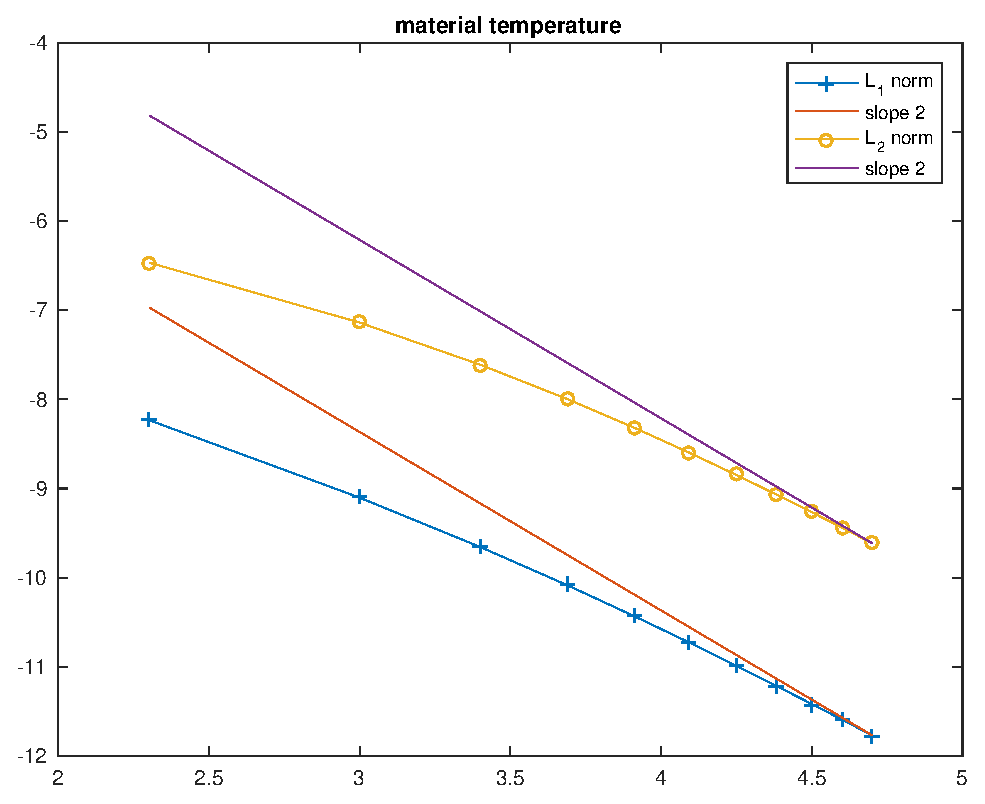
\includegraphics[width=\linewidth]{figures/cst-xs/mach_1p05_material_temperature_spline.eps}
    \caption{Material temperature.}\label{fig:mach-1p05-cst-xs-temp}
    \end{subfigure}
    ~
    \begin{subfigure}{0.5\textwidth}
    \centering
    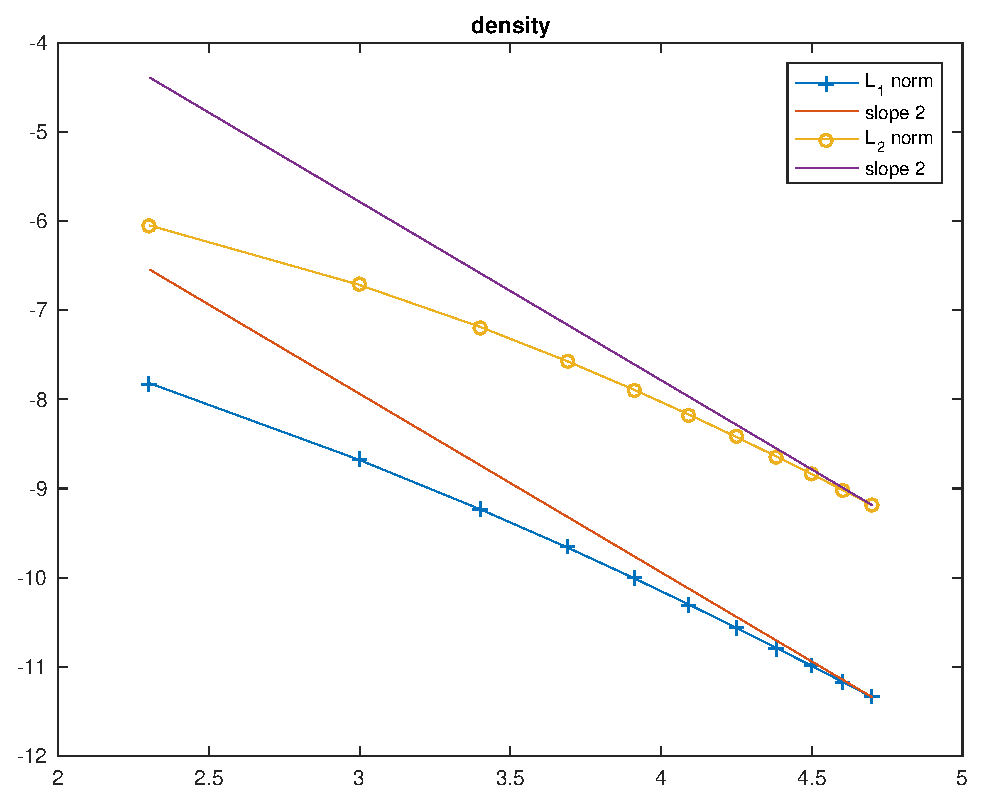
\includegraphics[width=\linewidth]{figures/cst-xs/mach_1p05_density_spline.eps}
    \caption{Material density.}\label{fig:mach-1p05-cst-xs-density}
    \end{subfigure}    
    
    \begin{subfigure}{0.5\textwidth}
    \centering
    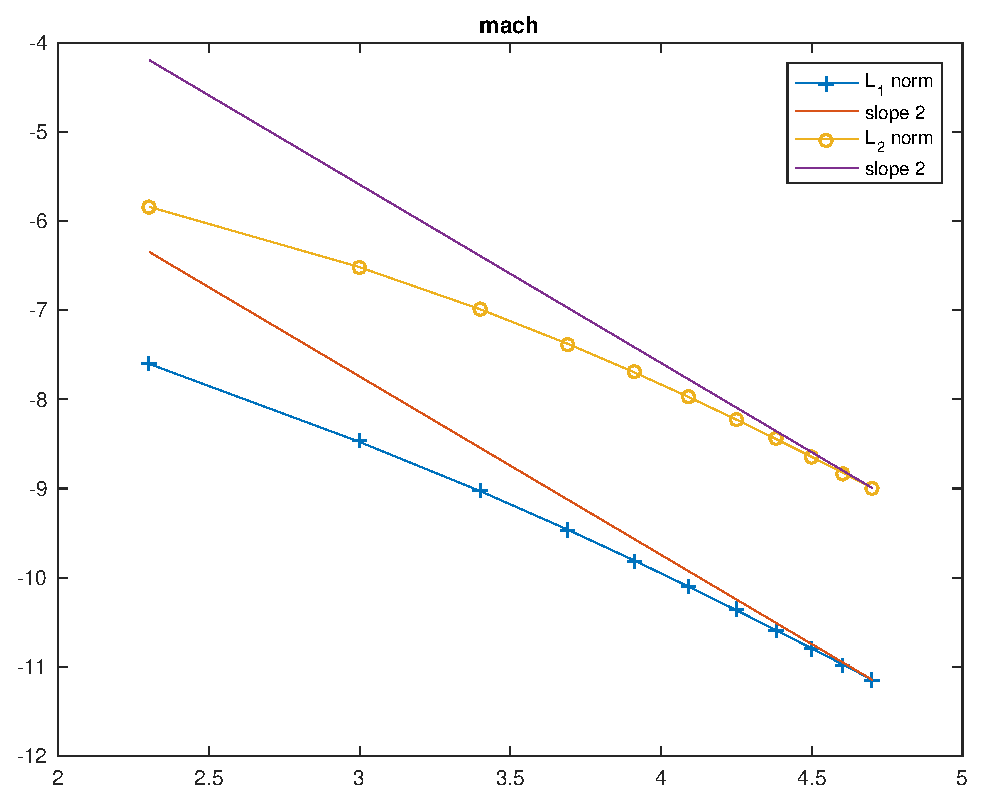
\includegraphics[width=\linewidth]{figures/cst-xs/mach_1p05_mach_spline.eps}
    \caption{Mach number.}\label{fig:mach-1p05-cst-xs-mach}
    \end{subfigure}
    ~
    \begin{subfigure}{0.5\textwidth}
    \centering
    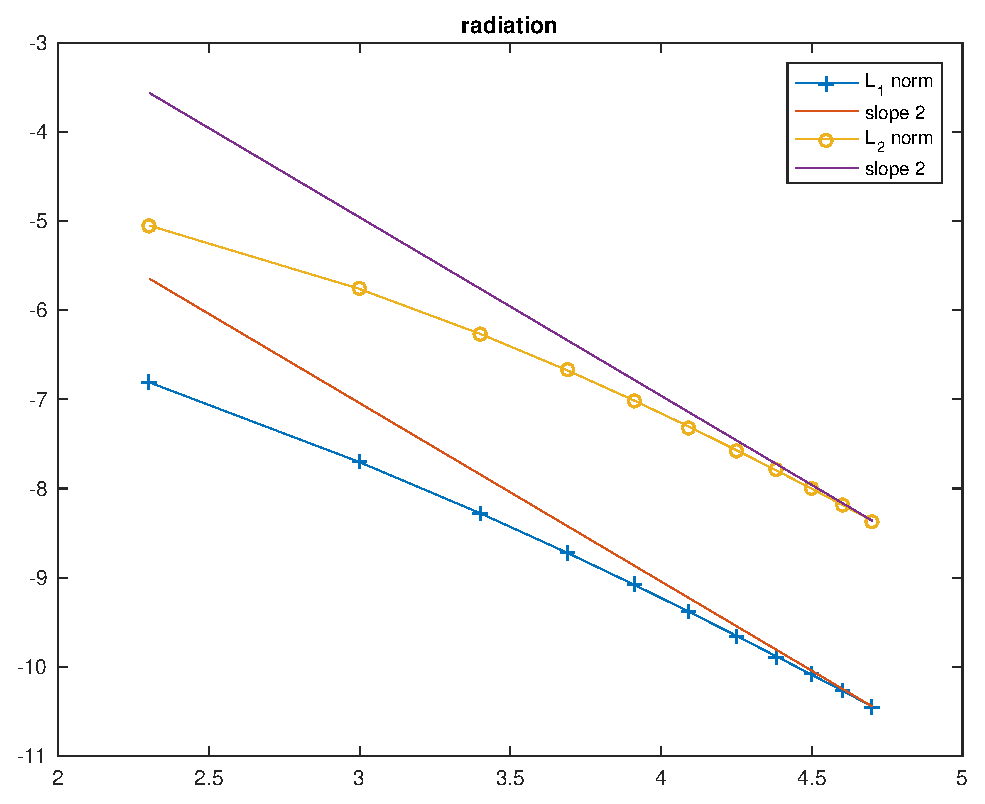
\includegraphics[width=\linewidth]{figures/cst-xs/mach_1p05_radiation_spline.eps}
    \caption{Radiation energy density.}\label{fig:mach-1p05-cst-xs-radiation}
    \end{subfigure}        
\caption{Convergence plots of the $L_1$ and $L_2$ error norms for Mach $1.05$ test.}\label{fig:mach-1p05-cst-xs}    
\end{figure}
%
%
%------------------------------------------------------------------
\subsection{Mach-3 shock test with constant opacities}\label{sec:mach-3-cst-xs}
%------------------------------------------------------------------
%
%\begin{table}[H]
%\caption{\label{tbl:table1} L$_1$ norms of the error for Mach 3 test.}
%\begin{center}
%\begin{tabular}{|c|c|c|c|c|c|c|c|c|c|}
%\hline
%\textbf{\# of cells} & $\mathbf{\rho}$ & \textbf{ratio} & $\mathbf{T}$ & \textbf{ratio} \\ \hline
%$100$ & $8.346\times 10^{6}$ & NA &  $29.675$ & NA \\ \hline
%$200$ & $3.436\times 10^{6}$ & $1.280$ &  $12.300$ & $1.271$ \\ \hline
%$400$ & $3.066\times10^{6}$ & $0.164$ &  $10.998$ & $0.161$ \\ \hline
%$800$ & $1.565\times 10^{6}$ & $0.969$ &  $5.689$ & $0.951$ \\ \hline
%$1600$ & $7.323\times 10^{5}$ & $1.096$ &  $2.741$ & $1.054$ \\ \hline
%$3200$ & $3.648\times 10^{5}$ & $1.005$ & $1.440$ & $0.928$ \\ \hline
%$6400$ & $1.823\times 10^{5}$ & $1.001$ & $0.794$ & $0.858$ \\ \hline
%\hline
%\textbf{\# of cells} & $\mathbf{\epsilon}$ & \textbf{ratio} &  $\mathbf{Mach}$ & \textbf{ratio} \\ \hline
%$100$ & $7.470\times 10^{6}$ & NA & $1.458\times 10^6$ & NA	\\ \hline
%$200$ & $3.075\times 10^{6}$ & $1.280$ & $6.001\times 10^5$ & $1.280$	\\ \hline
%$400$ & $2.744\times 10^{6}$ & $0.164$ & $5.3555\times 10^5$ & $0.164$	\\ \hline
%$800$ & $1.401\times 10^{6}$ & $0.969$ & $2.734\times 10^5$ & $0.969$	\\  \hline
%$1600$&$6.555\times 10^{5}$ & $1.096$ & $1.279\times 10^5$ & $1.096$ \\ \hline 
%$3200$ & $3.266\times10^{5}$  & $1.005$ & $6.372\times 10^4$ & $1.005$ \\ \hline   
%$6400$ & $1.632\times 10^{5}$  & $1.000$ & $3.184\times10^4$ & $1.001$ \\ \hline   
%\end{tabular}  
%\end{center}
%\end{table}
%%
%\begin{table}[H]
%\caption{\label{tbl:table1} L$_2$ norms of the error for Mach 3 test.}
%\begin{center}
%\begin{tabular}{|c|c|c|c|c|c|c|c|c|c|}
%\hline
%\textbf{\# of cells} & $\mathbf{\rho}$ & \textbf{ratio} & $\mathbf{T}$ & \textbf{ratio} \\ \hline
%$100$ & $6.087\times 10^{8}$ & NA &  $29.675$ & NA \\ \hline
%$200$ & $3.177\times 10^{8}$ & $1.280$ &  $12.300$ & $0.938$ \\ \hline
%$400$ & $3.827\times10^{8}$ & $0.164$ &  $10.998$ & $0.269$ \\ \hline
%$800$ & $2.742\times 10^{8}$ & $0.969$ &  $5.689$ & $0.481$ \\ \hline
%$1600$ & $1.811\times 10^{8}$ & $1.096$ &  $2.741$ & $0.599$ \\ \hline
%$3200$ & $1.275\times 10^{8}$ & $1.005$ & $1.440$ & $0.506$ \\ \hline
%$6400$ & $9.011\times 10^{7}$ & $1.001$ & $0.794$ & $0.501$ \\ \hline
%\hline
%\textbf{\# of cells} & $\mathbf{\epsilon}$ & \textbf{ratio} &  $\mathbf{Mach}$ & \textbf{ratio} \\ \hline
%$100$ & $5.448\times 10^{8}$ & NA & $1.063\times 10^9$ & NA	\\ \hline
%$200$ & $2.843\times 10^{8}$ & $0.938$ & $5.548\times 10^8$ & $0.938$	\\ \hline
%$400$ & $3.426\times 10^{8}$ & $0.269$ & $6.685\times 10^8$ & $0.269$	\\ \hline
%$800$ & $2.454\times 10^{8}$ & $0.481$ & $4.789\times 10^8$ & $0.481$	\\  \hline
%$1600$&$1.621\times 10^{8}$ & $0.599$ & $3.162\times 10^8$ & $0.599$ \\ \hline 
%$3200$ & $1.141\times10^{8}$  & $0.506$ & $2.227\times 10^8$ & $0.506$ \\ \hline   
%$6400$ & $8.064\times 10^{7}$  & $0.501$ & $1.574\times10^8$ & $0.501$ \\ \hline   
%\end{tabular}  
%\end{center}
%\end{table}
%
For this test, the inlet Mach number is set to $3$ and the total and absorption cross sections are assumed constant. The initial conditions are computed from the four non-dimensional numbers $\mathbb{P}_\infty=10^{-4}$, $M=3$, $\mathbb{\Sigma}=10^6$ and $\mathbb{\Lambda}=1$ which yields an opacityof $577.35 \ cm^{-1}$. The steady-state numerical results for the material density, the material and radiation temperatures, and the viscosity coefficient $\kappa$ are presented in \fig{fig:mach-3-cst-xs-dens}, \fig{fig:mach-3-cst-xs-temp} and \fig{fig:mach-3-cst-xs-visc}, respectively, along with the semi-analytical solutions from \cite{ferguson}.
\begin{figure}[H]
    \centering
    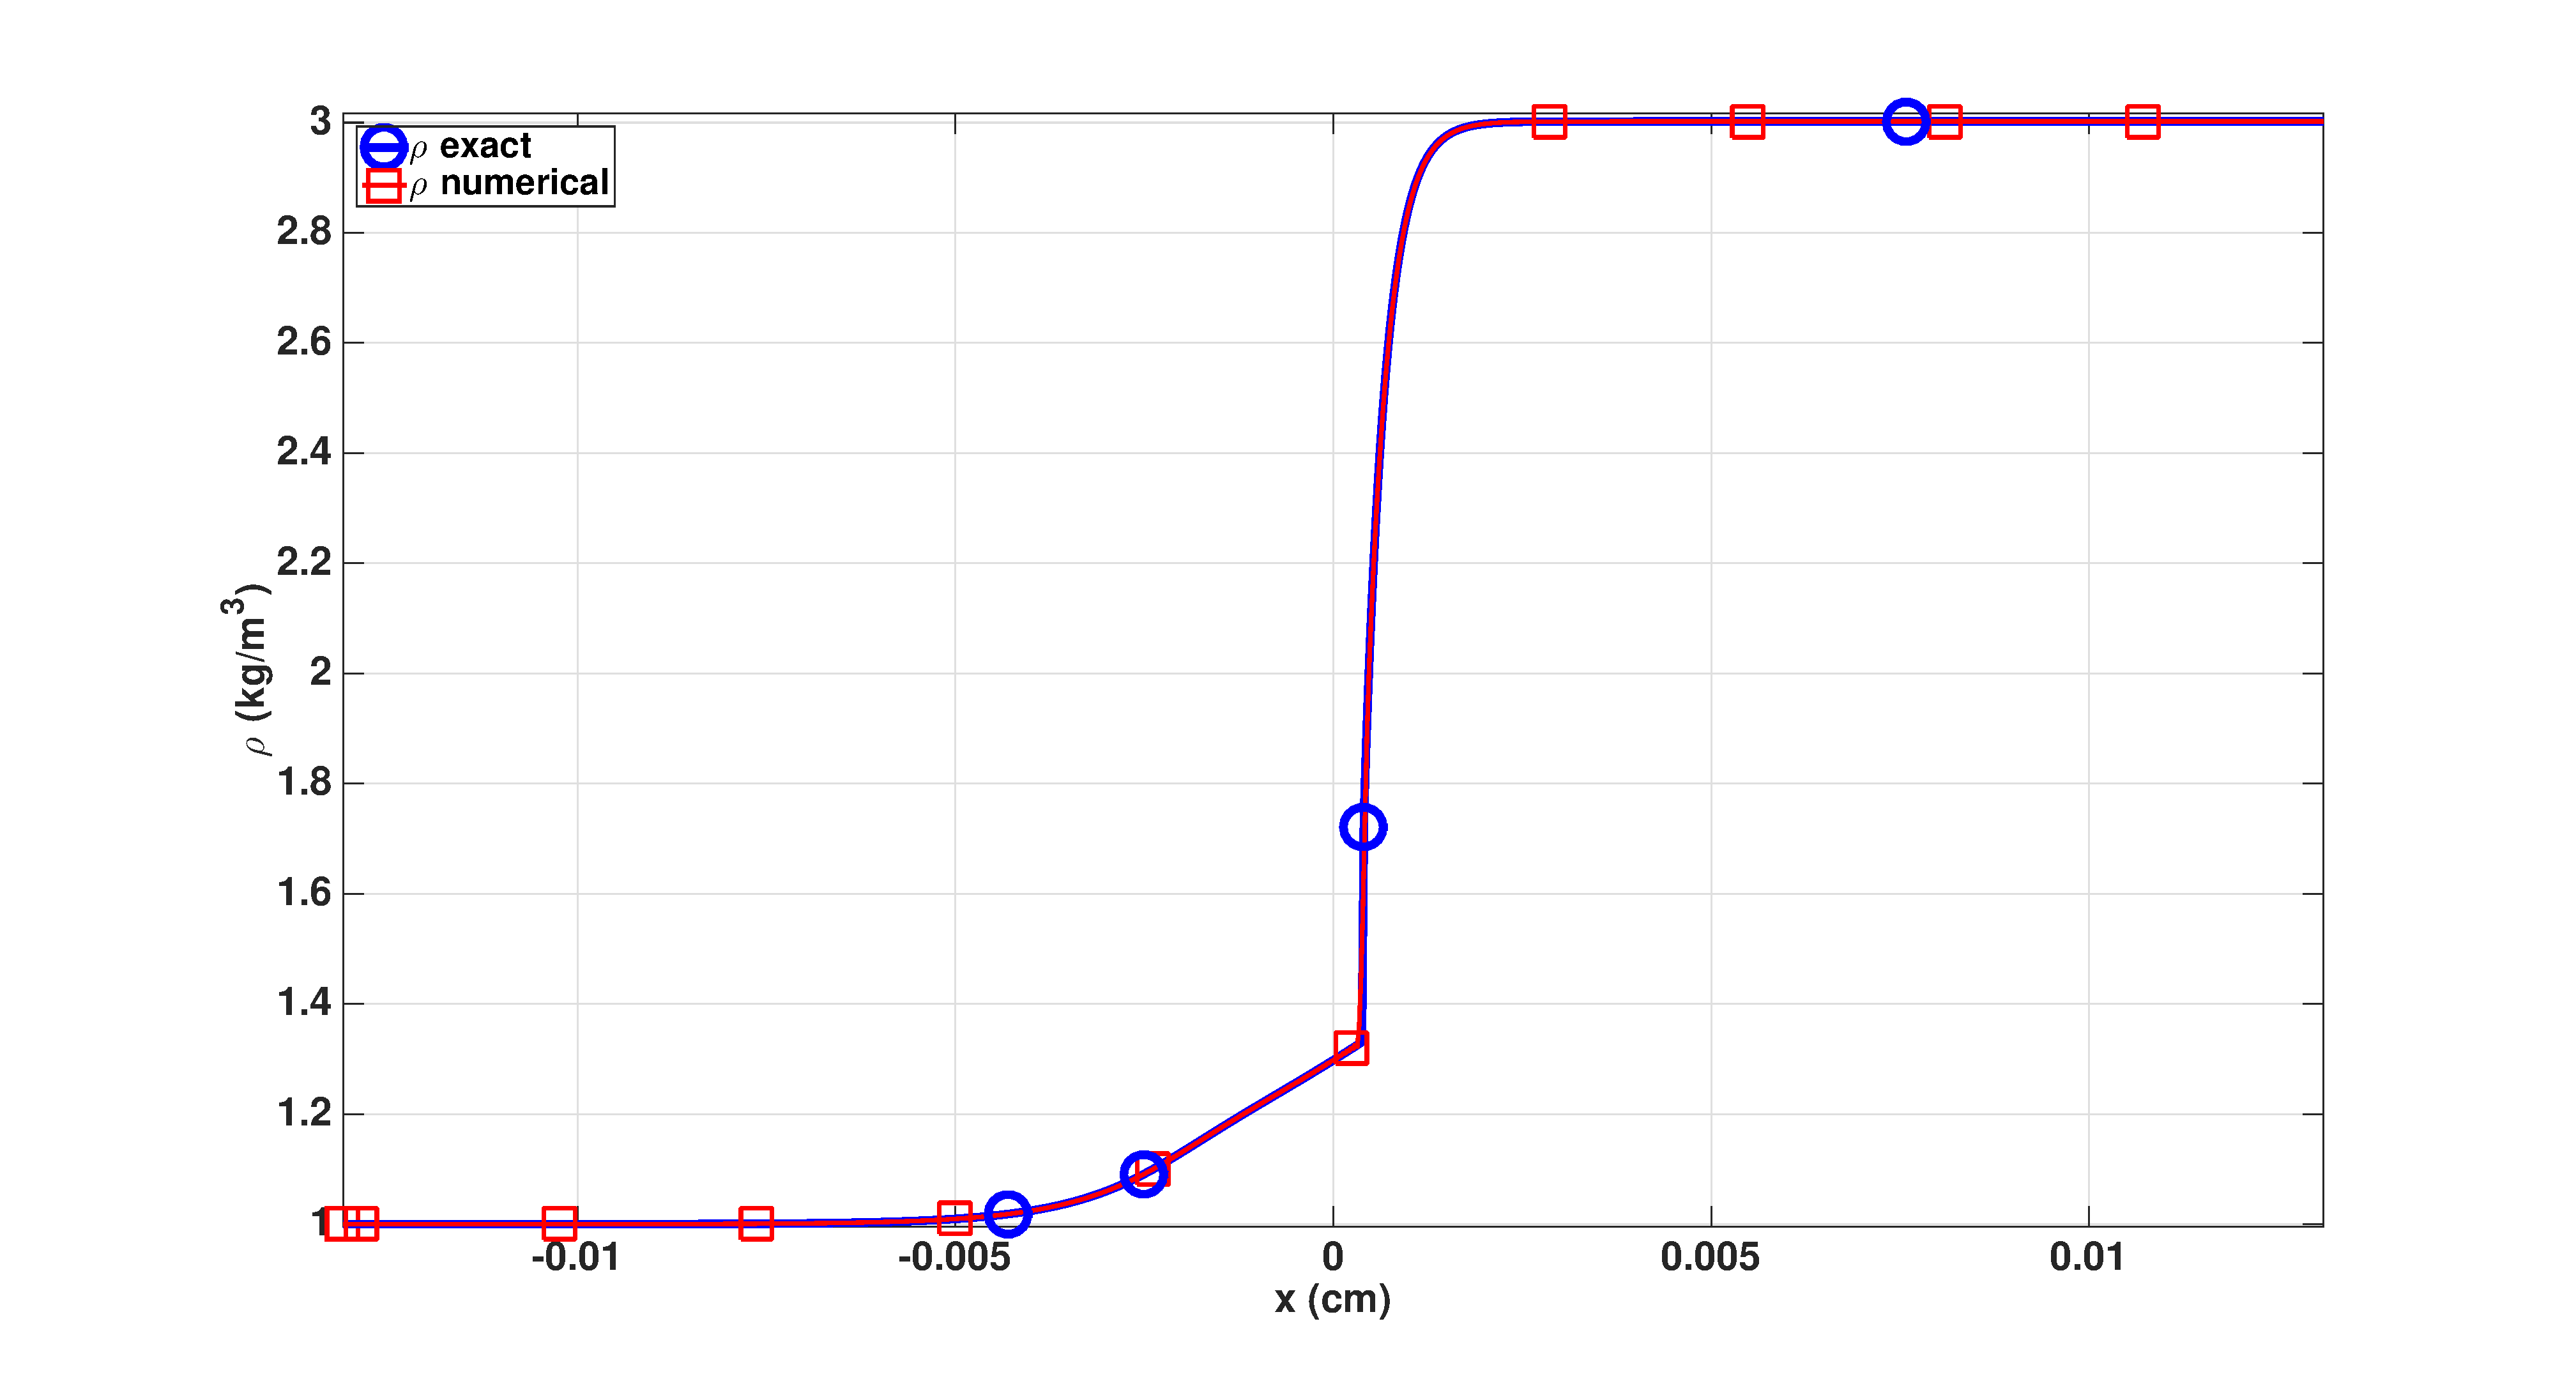
\includegraphics[width=\textwidth]{figures/cst-xs/mach_3_cst_xs_nel_1000_density.eps}
%    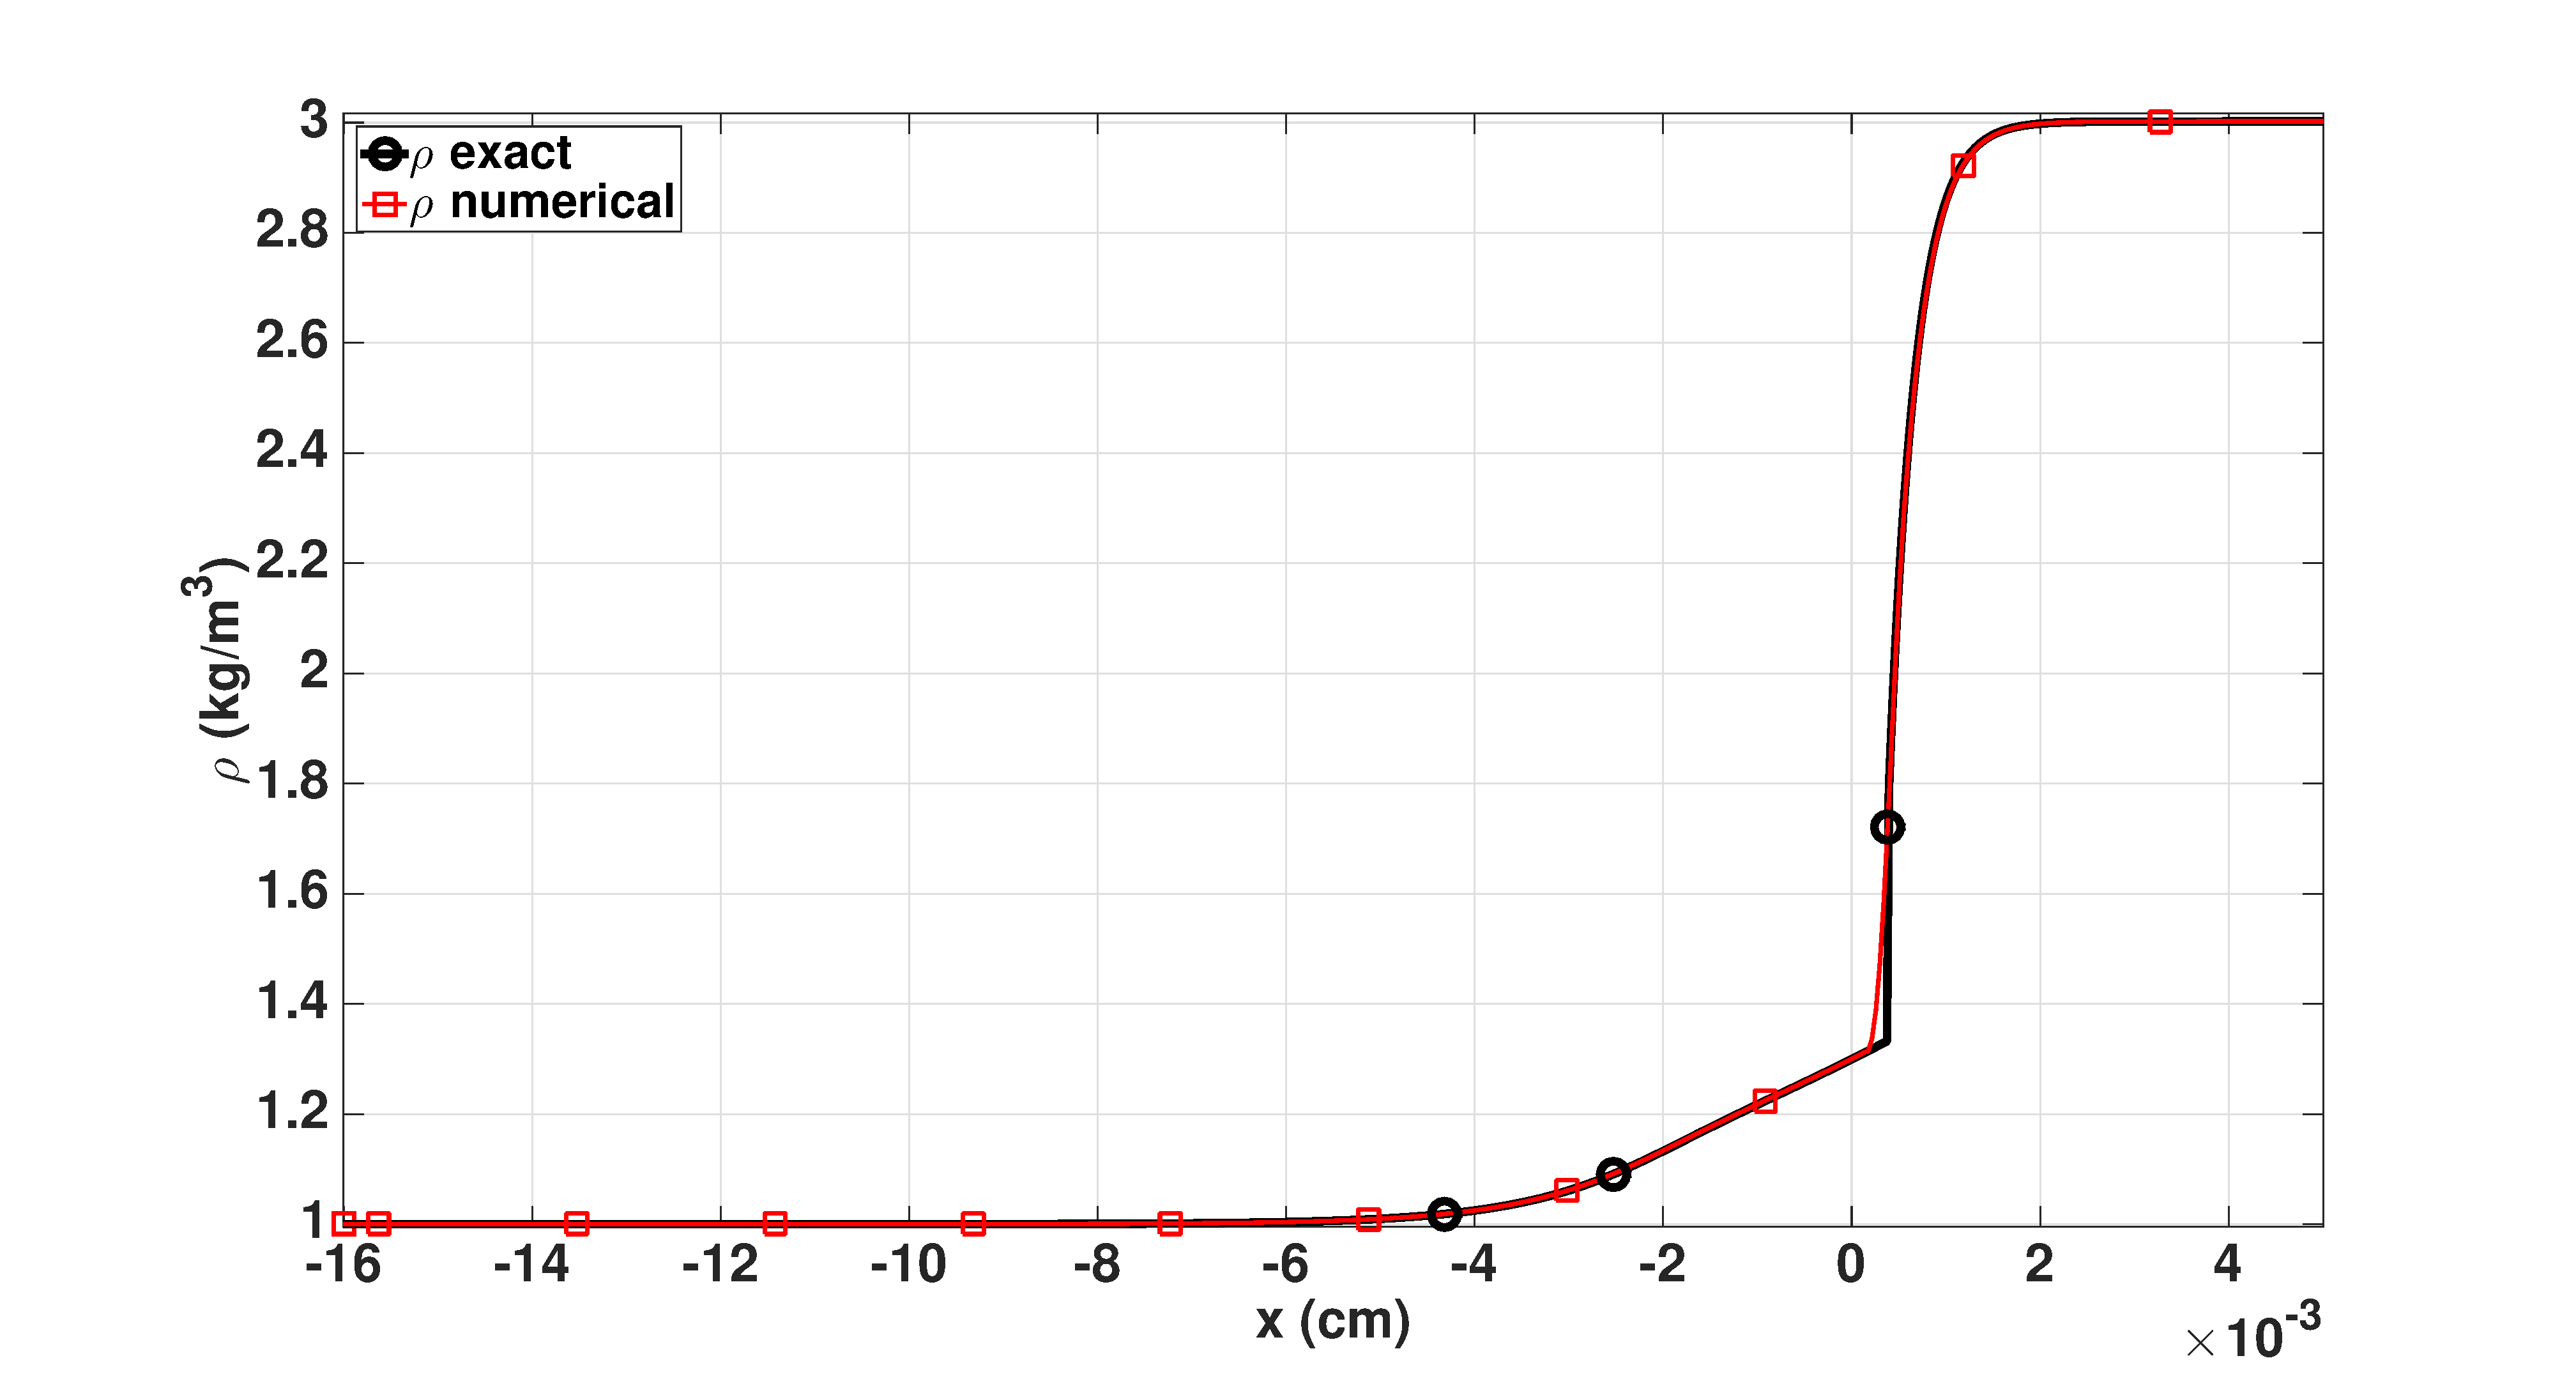
\includegraphics[width=\textwidth]{figures/cst-xs/mach_3_cst_xs_nel_500_density.eps}    
    \caption{Steady-state material density for the Mach-3 shock test.}\label{fig:mach-3-cst-xs-dens}
\end{figure}
%
The material density plotted in \fig{fig:mach-3-cst-xs-dens} shows good agreement with the semi-analytical solution: the shock located around $x=0 \ cm$ is well resolved and does not display any instability.
%
\begin{figure}[H]
    \centering
    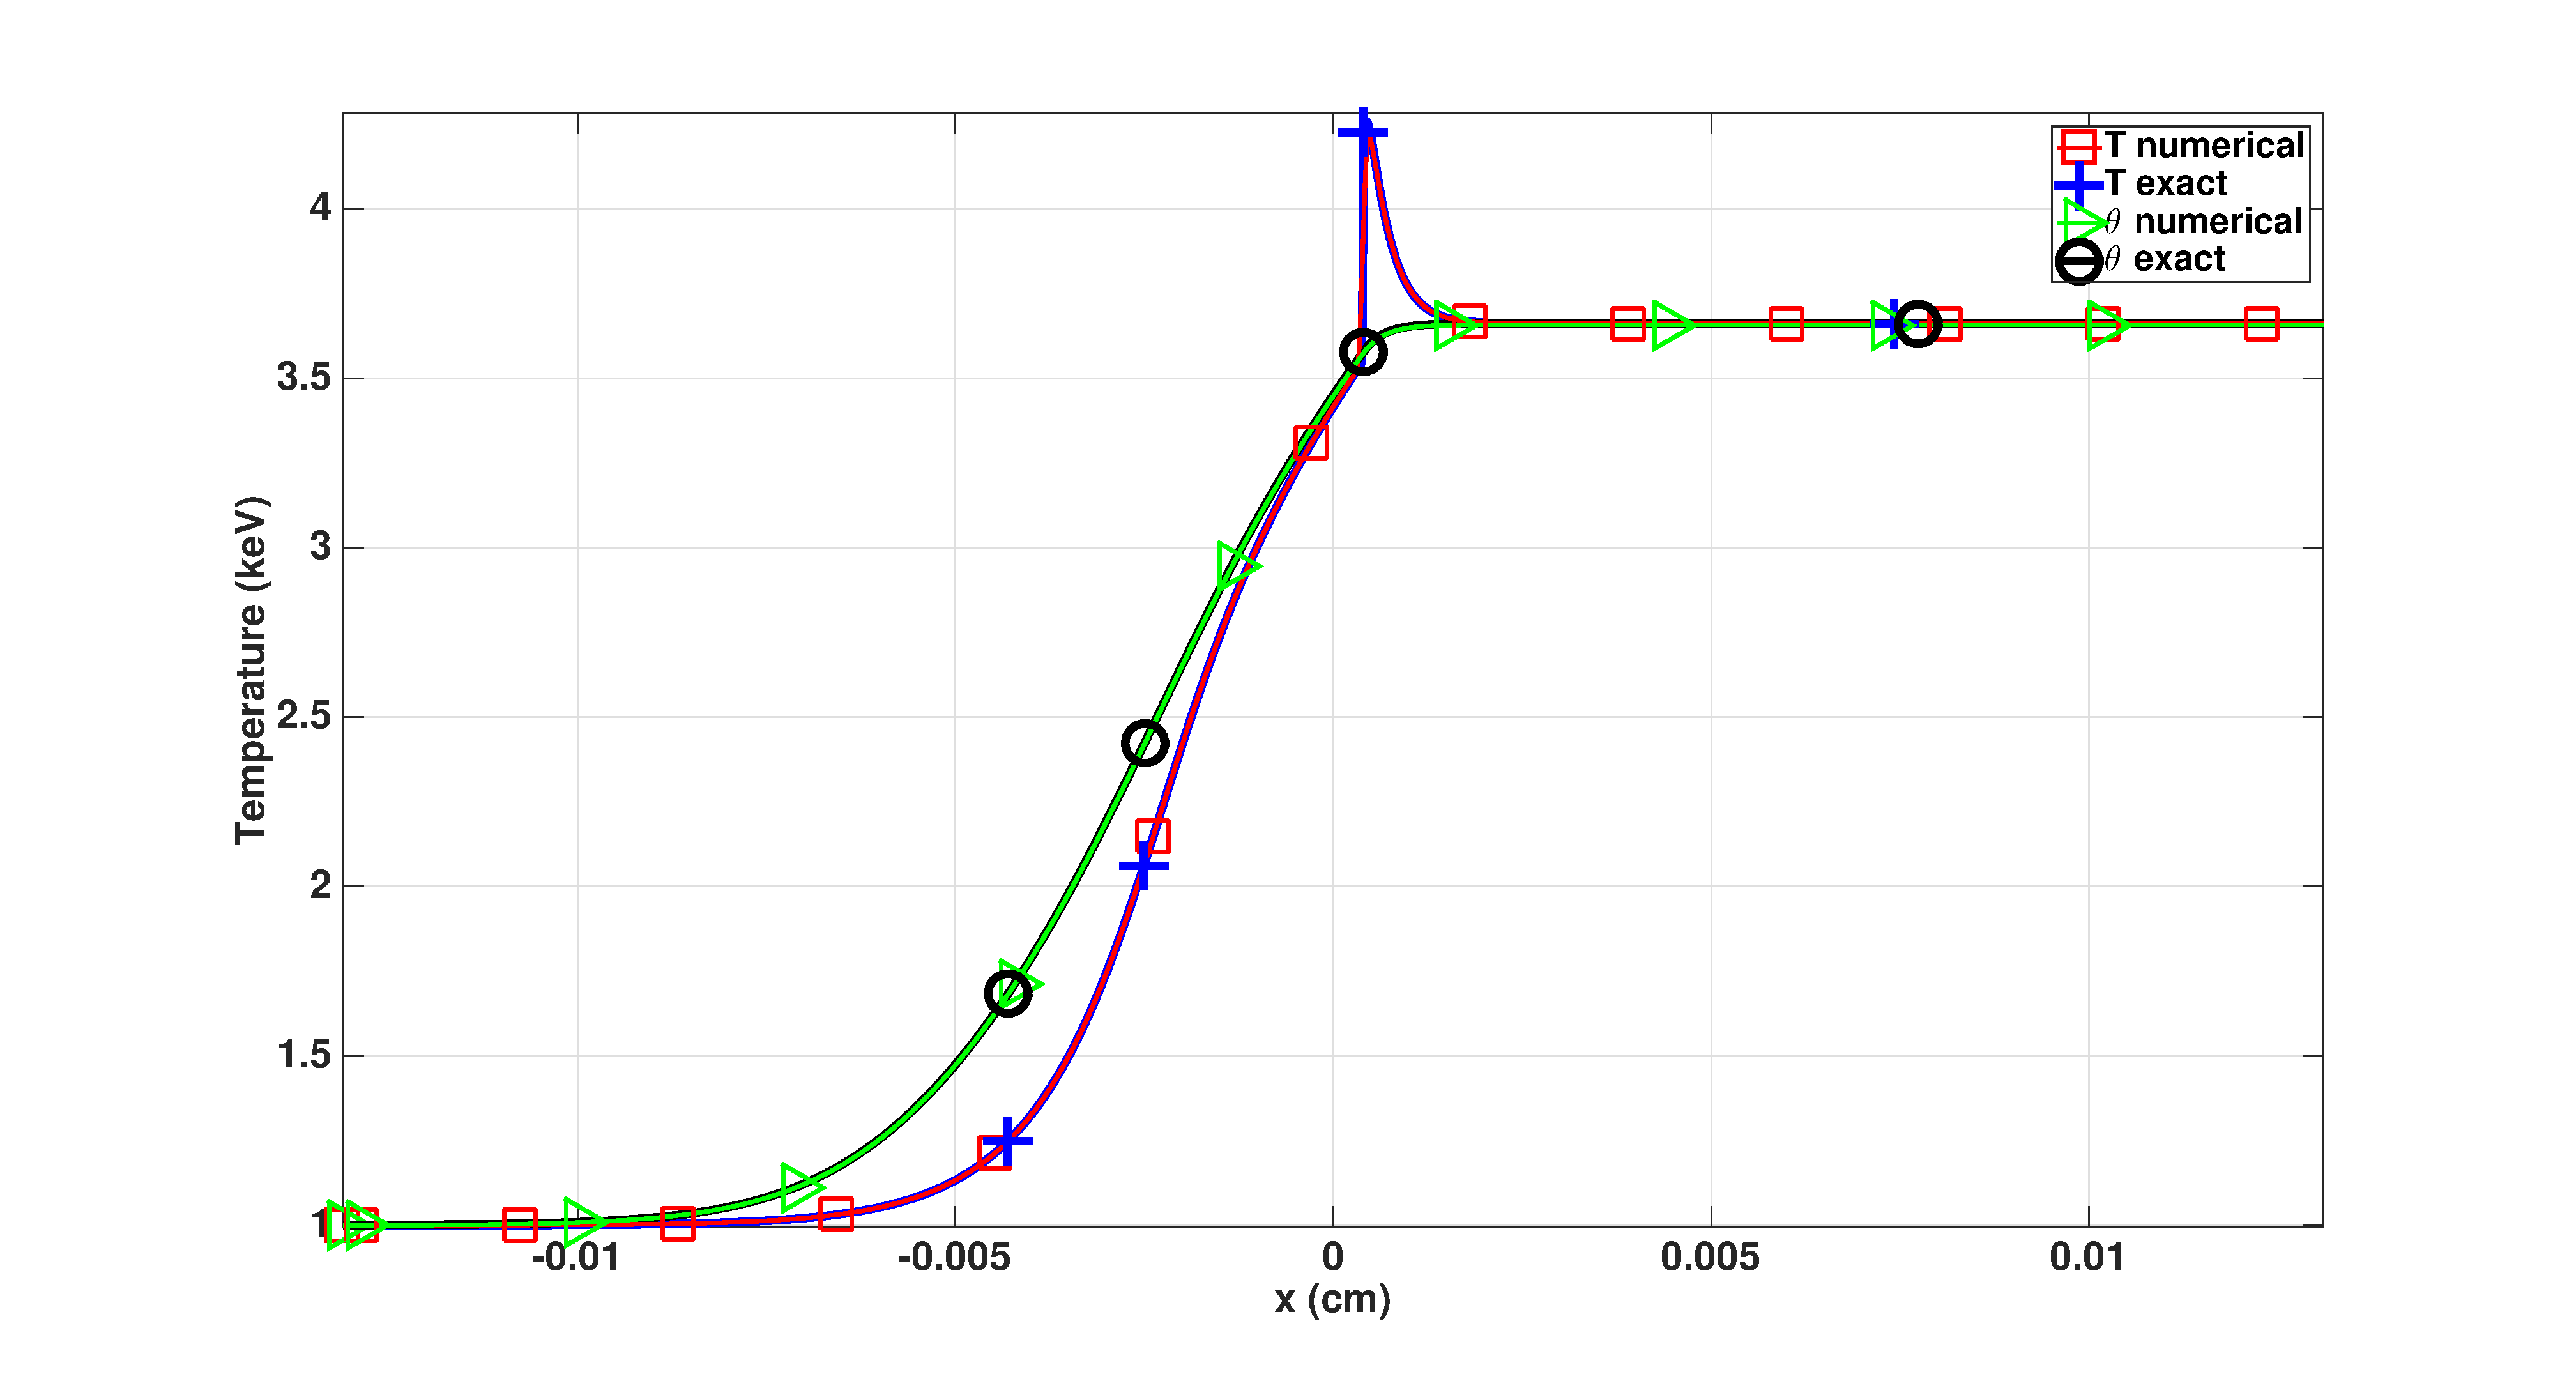
\includegraphics[width=\textwidth]{figures/cst-xs/mach_3_cst_xs_nel_1000_temperature.eps}
%    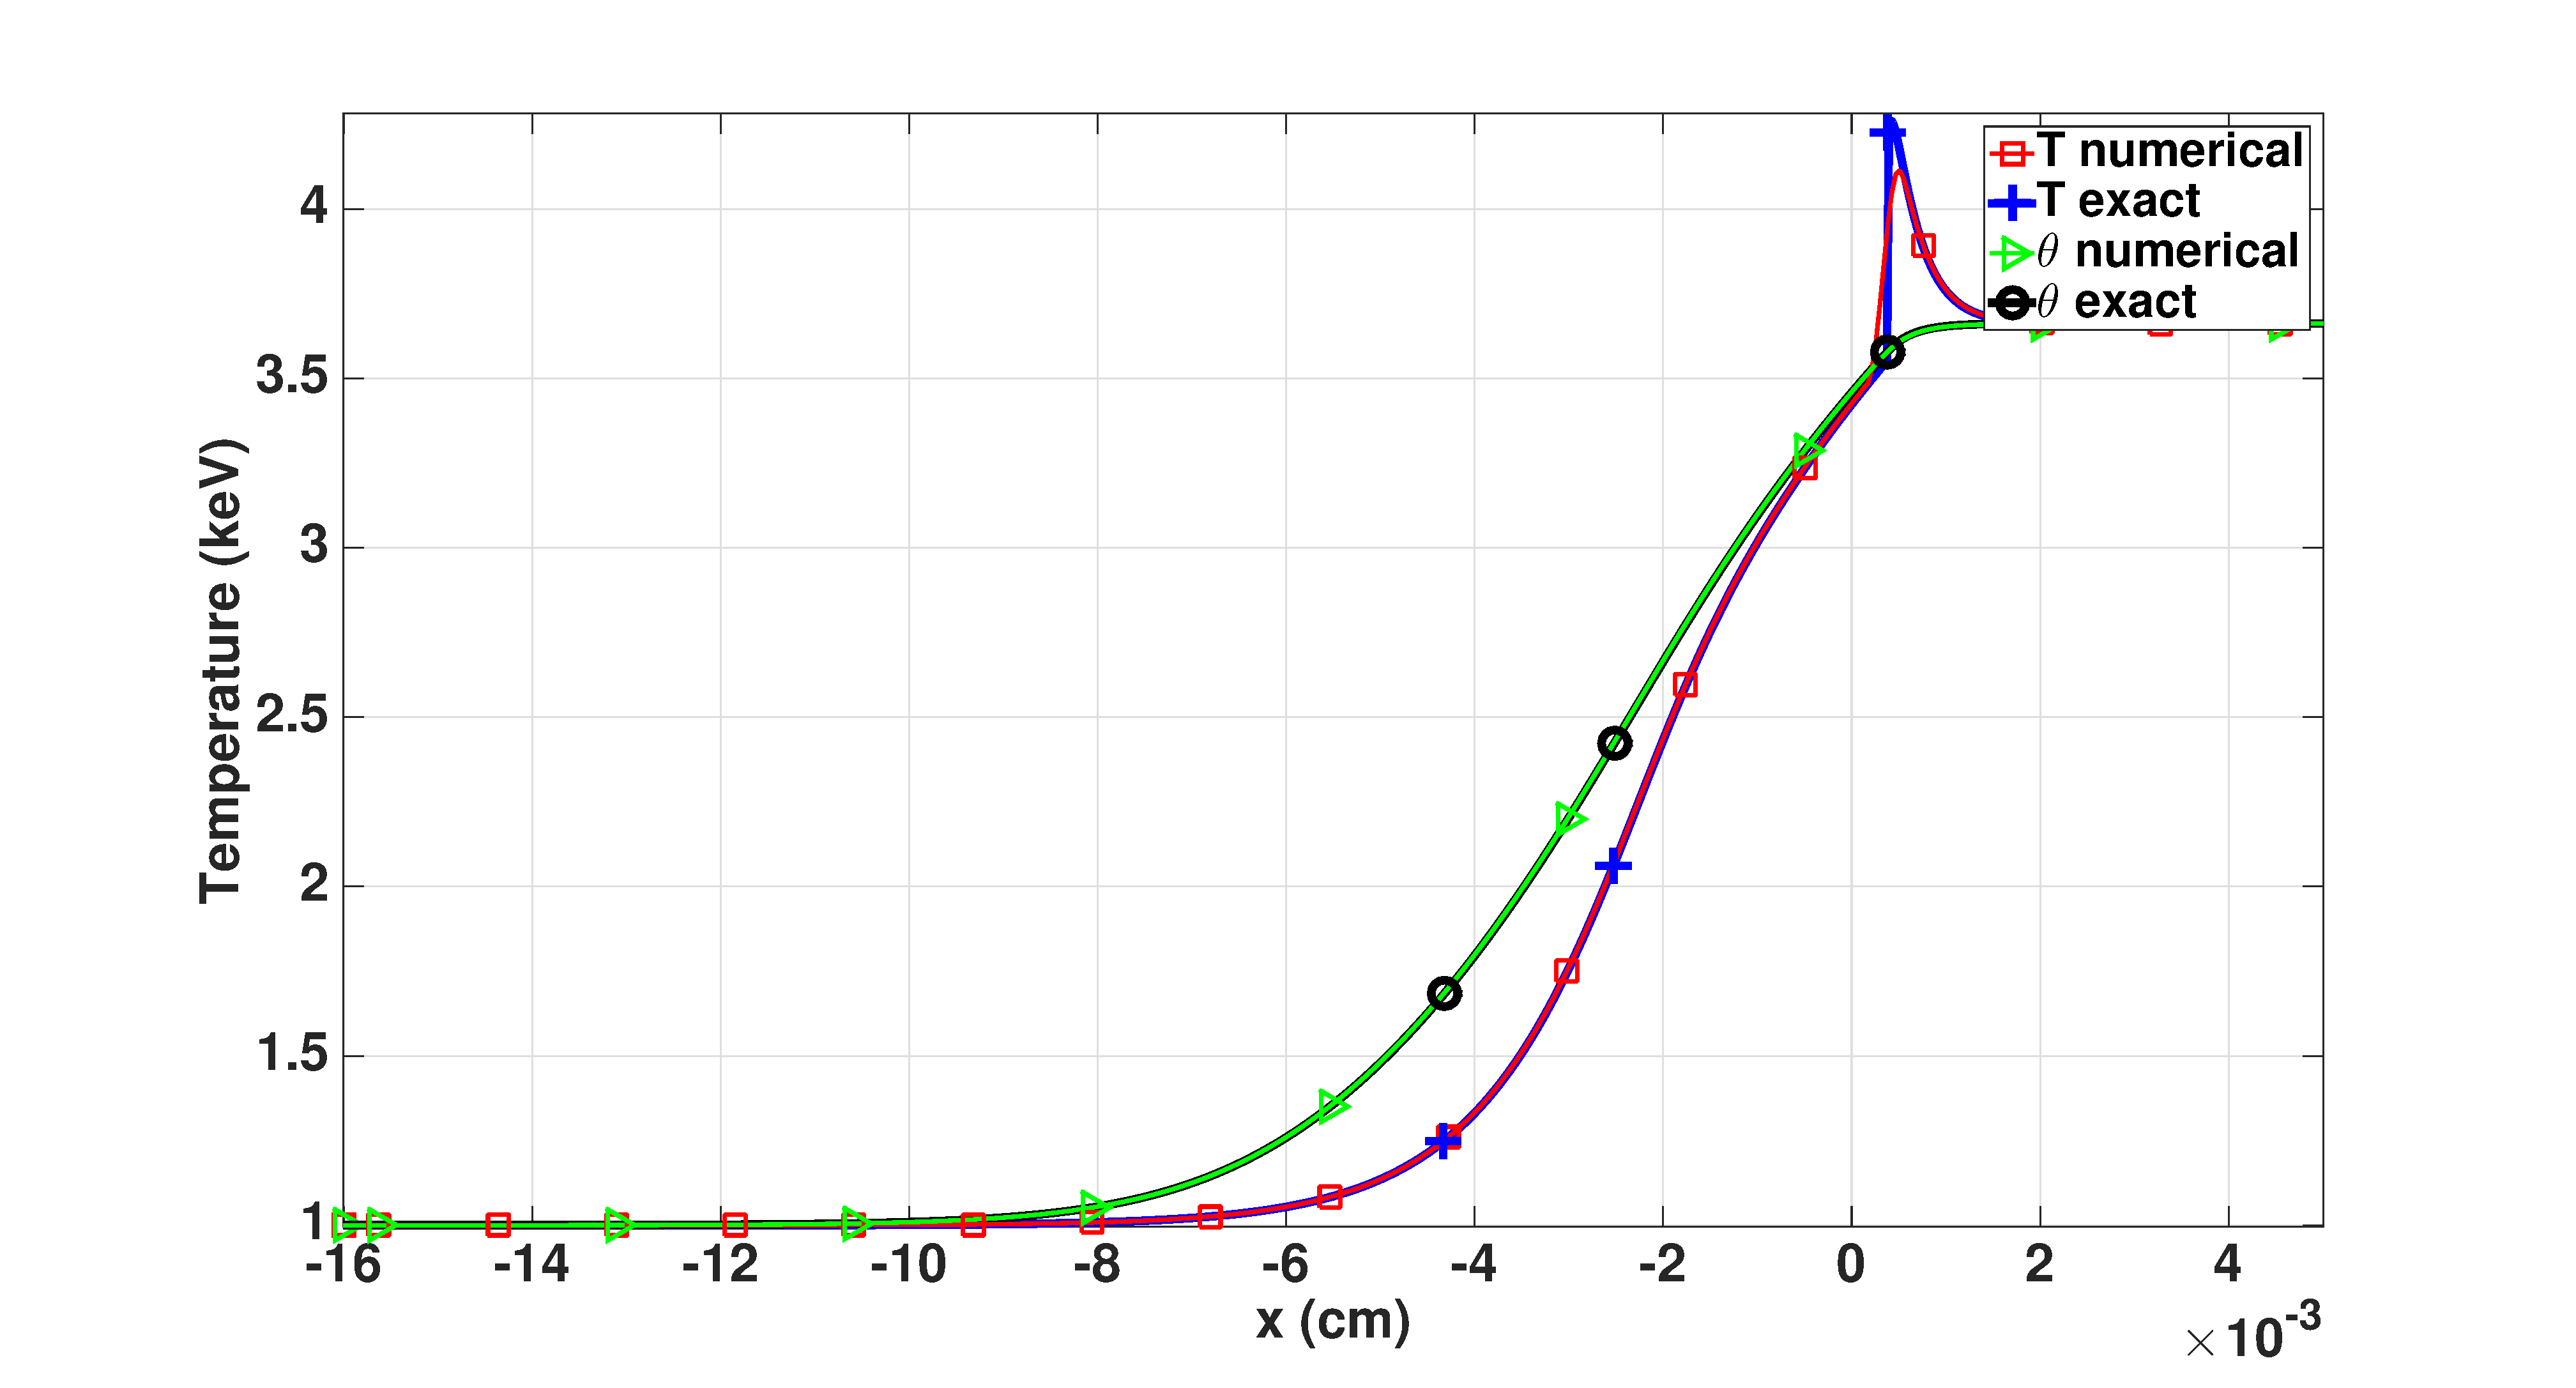
\includegraphics[width=\textwidth]{figures/cst-xs/mach_3_cst_xs_nel_500_temperature.eps}    
    \caption{Steady-state material and radiation temperatures for the Mach-3 shock test.}\label{fig:mach-3-cst-xs-temp}
\end{figure}
%
In \fig{fig:mach-3-cst-xs-temp}, the material temperature shows a Zeldovich's peak around $x=0 \ cm$ that corresponds to the shock position in the material density profile (see \fig{fig:mach-3-cst-xs-dens}). The radiation temperature remains smooth even in the vicinity of the peak because of the diffusion term $ \partial_x \left( \frac{c}{3 \sigma_t} \partial_x \epsilon \right)$ in the radiation equation (\eqt{eq:GRHrad}). Both the material and radiation temperature profiles show good agreement with the semi-analytical solutions.
%
\begin{figure}[H]
    \centering
    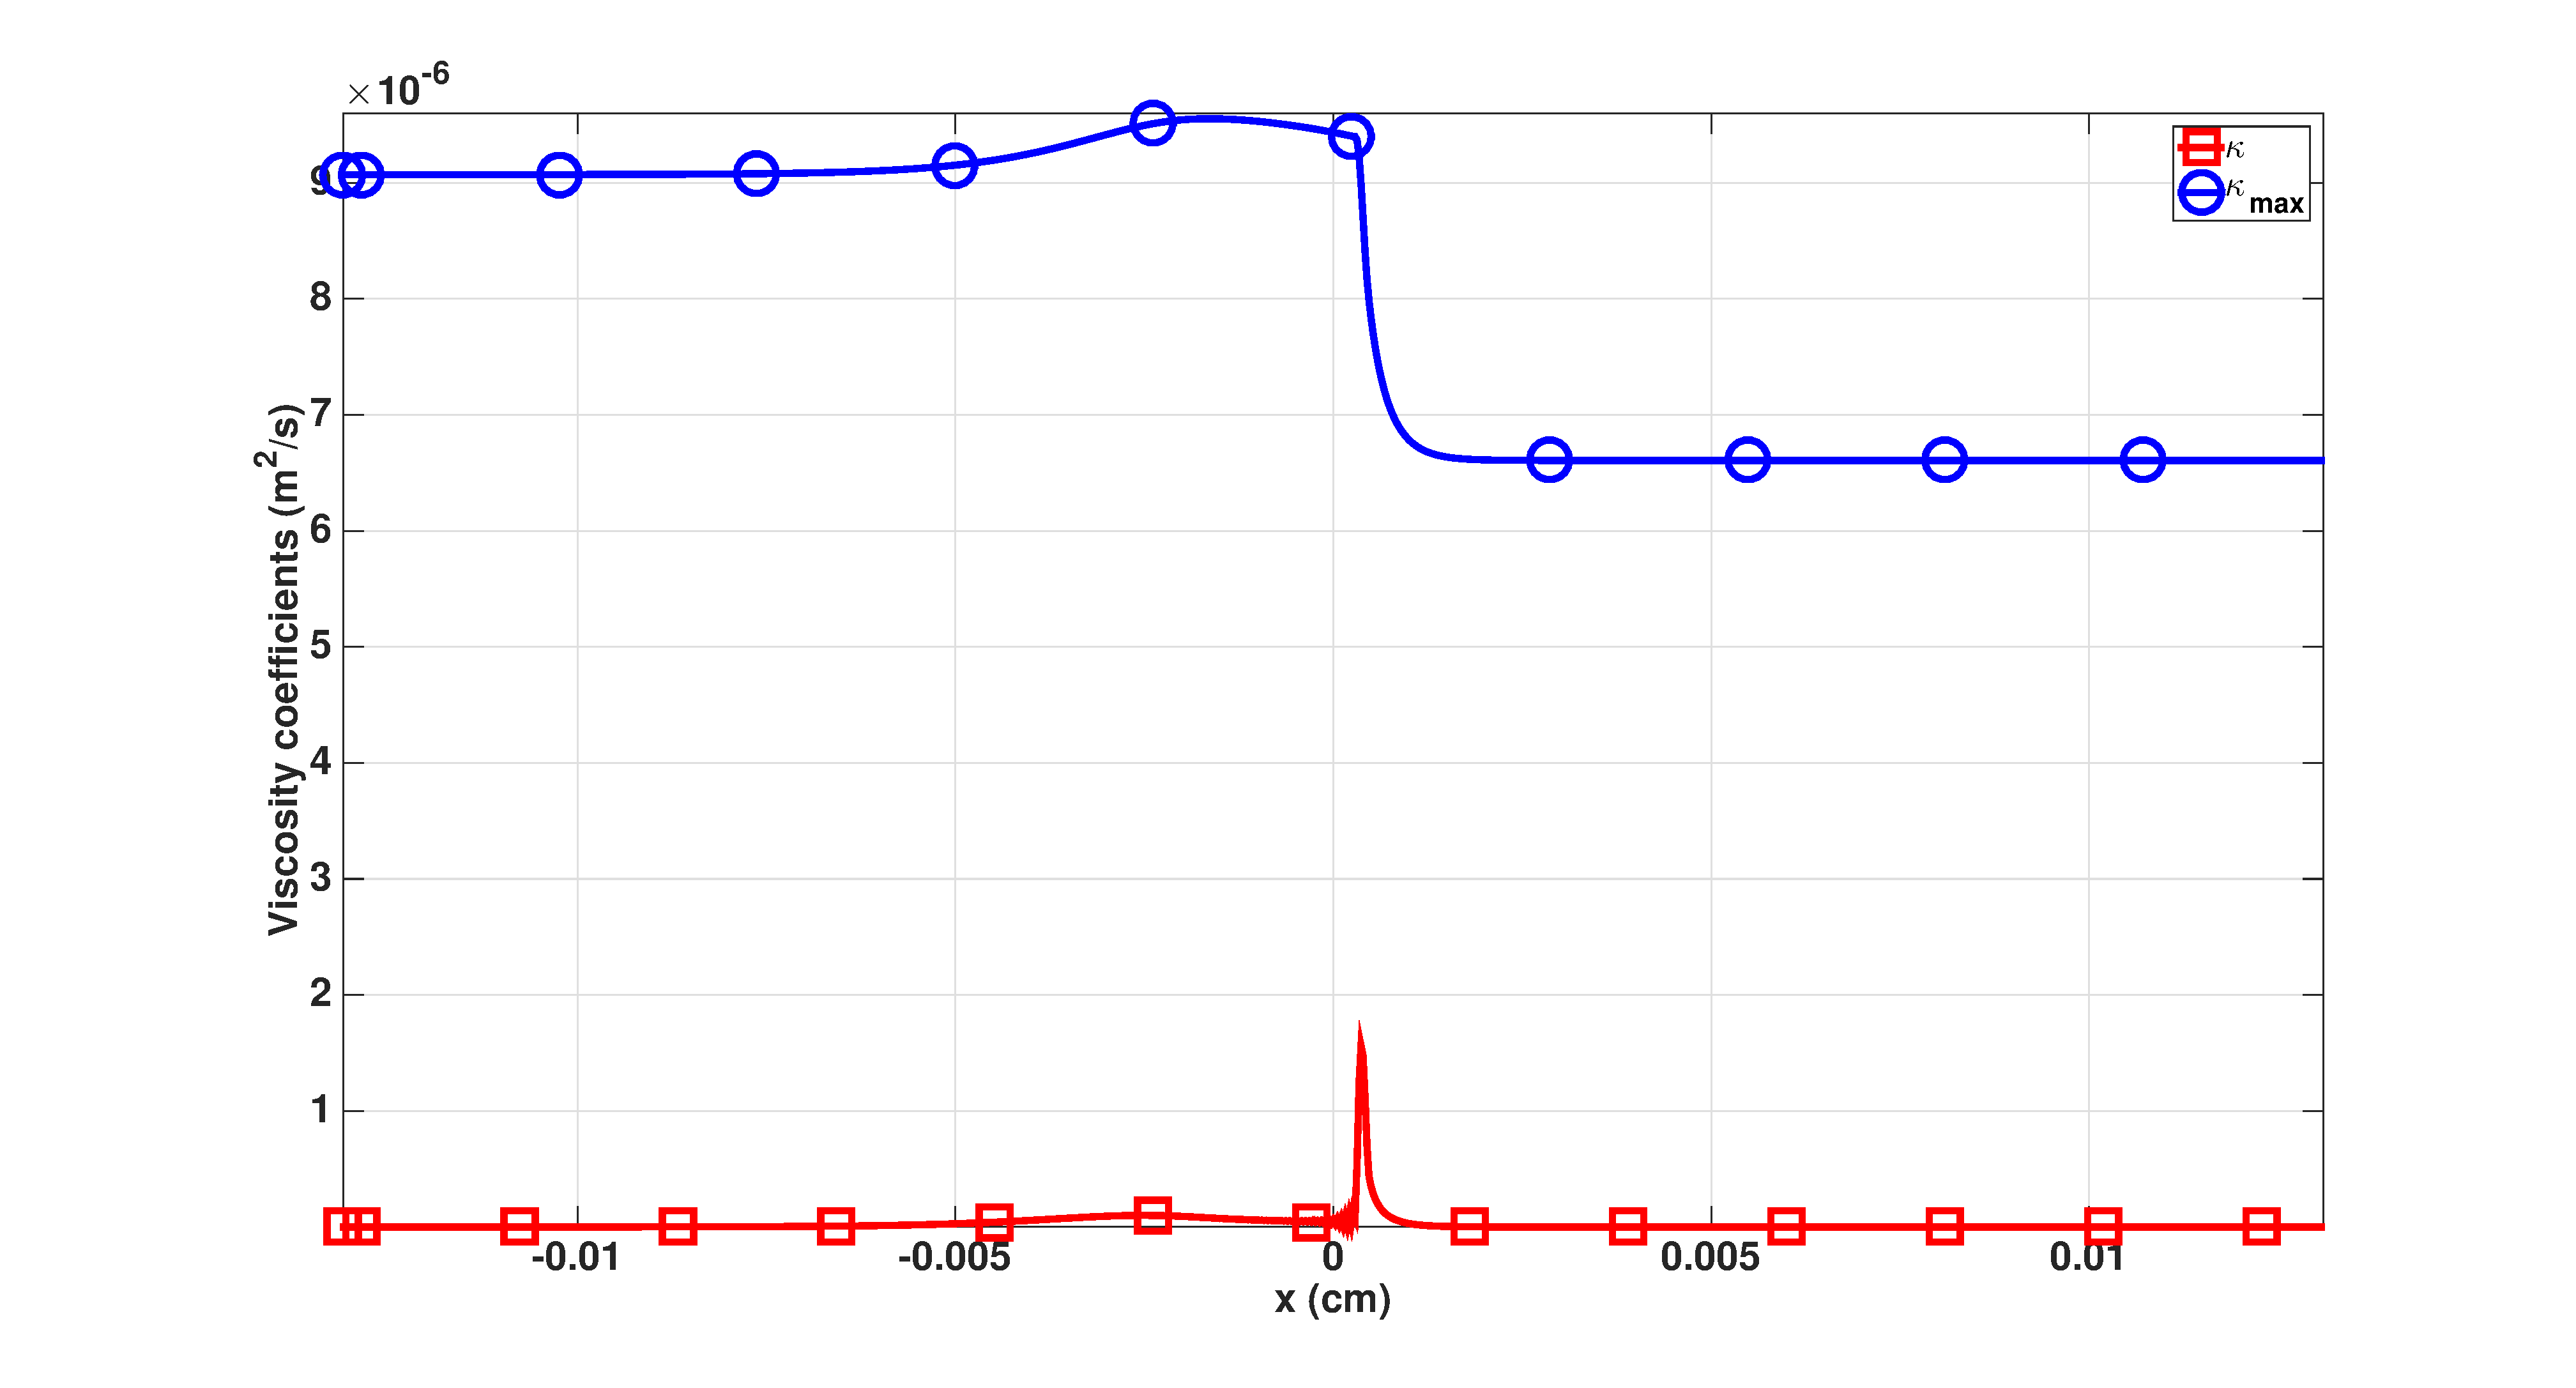
\includegraphics[width=\textwidth]{figures/cst-xs/mach_3_cst_xs_nel_1000_viscosity.eps}
%    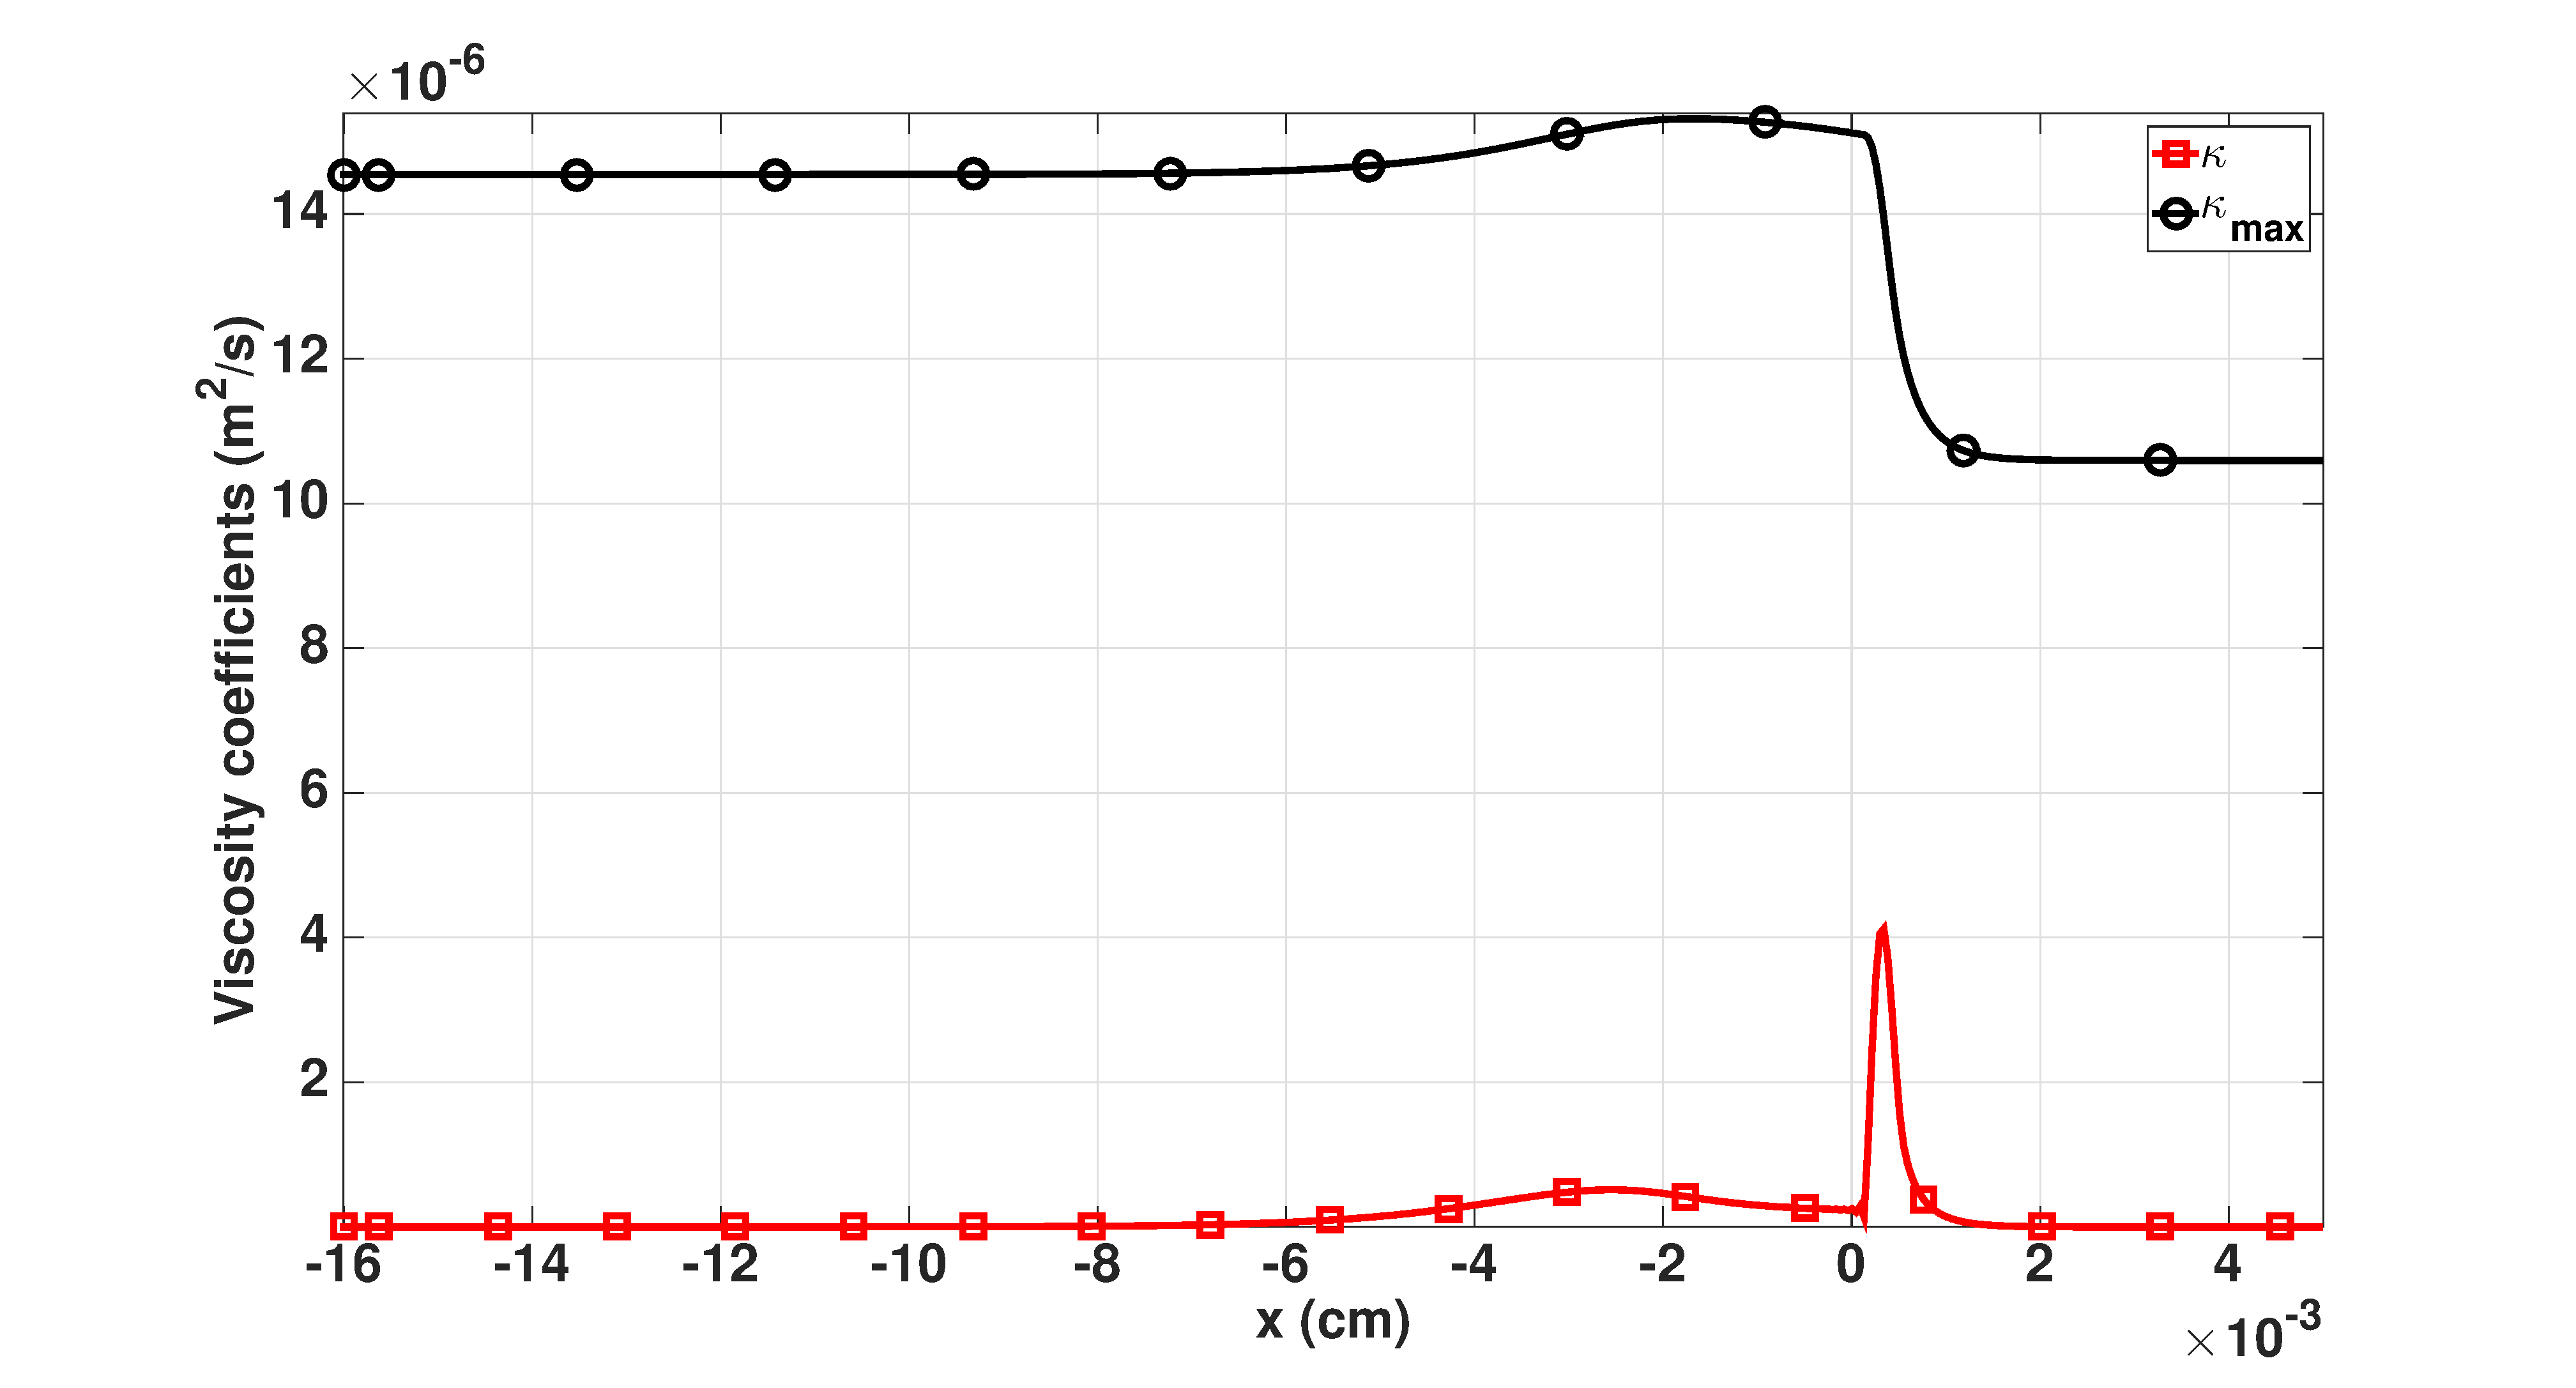
\includegraphics[width=\textwidth]{figures/cst-xs/mach_3_cst_xs_nel_500_viscosity.eps}    
    \caption{Steady-state artificial viscosity coefficient for the Mach-3 shock test.}\label{fig:mach-3-cst-xs-visc}
\end{figure}
%
The viscosity coefficients $\kappa$ displays a peak in the vicinity of the shock around $x=0 \ cm$ as shown in \fig{fig:mach-3-cst-xs-visc}: this behavior is conformed to the definition of the viscosity coefficient $\kappa$ that is set proportional to the local entropy residual (see \eqt{eq:equation12}). We note that the viscosity coefficient $\kappa$ does not saturate to the first-order, over-dissipative viscosity coefficient $\kappa_{max}$ but still efficiently stabilizes the numerical solution. We have shown
in \sct{sec:VR_new} that the relaxation source terms were entropy-producing; thus it may not be necessary for the entropy viscosity to saturate to the first-order viscosity at shock locations.
%
%------------------------------------------------------------------
\subsection{Mach-3 shock test with temperature-dependent opacities}\label{sec:mach-3-no-cst-xs}
%------------------------------------------------------------------
%
%\tcb{We need a reference for this test. I have the report that was emailed by Dr Morel to me but I am not sure this is sufficient} \\
We now consider a Mach 3 test in a pure absorber material with the same non-dimensional numbers as in \sct{sec:mach-3-cst-xs} but the opacities now depend on the material properties, i.e, the density $\rho$ and the material temperature $T$. An expression of the \emph{dimensional} form of the density- and  temperature-dependent opacities is given in \eqt{eq:opacity}:
% there was a tilde sigma here, why?
%
\begin{equation}\label{eq:opacity}
\sigma_a = \sigma_t = \rho \frac{7216.875}{T^{\frac{2}{5}}}\, ,
\end{equation}
%
This simulation aims at exercising the entropy viscosity method with opacity functions that exhibit strong variations in the shock region. From a theoretical perspective, as proven in \sct{sec:def-visc-coeff}, the entropy inequality should nonetheless hold, meaning that the viscous regularization should efficiently stabilize any discontinuity or shock that could form in the numerical solution. 

The test is run until a steady state is reached. Numerical results for the material density and the material and radiation temperatures are presented and plotted against semi-analytical solutions in \fig{fig:mach-3-dpt-xs-dens} and \fig{fig:mach-3-dpt-xs-temp}, respectively. The values of the total/absorption opacity is given in \eqt{fig:mach-3-dpt-xs-xs}. We also provide the viscosity coefficient profiles at steady state in \fig{fig:mach-3-dpt-xs-visc}.
%\begin{itemize}
%\item numerical results using definition of the viscosity coefficient provided in previous section: density, temperature, opacity and viscosity coefficient profiles.
%\item eyeball convergence study when refining the mesh.
%\item investigate the influence of the jumps in the definition of the viscosity coefficients: run the same numerical test with and without jumps.
%\end{itemize}
%
\begin{figure}[H]
    \centering
    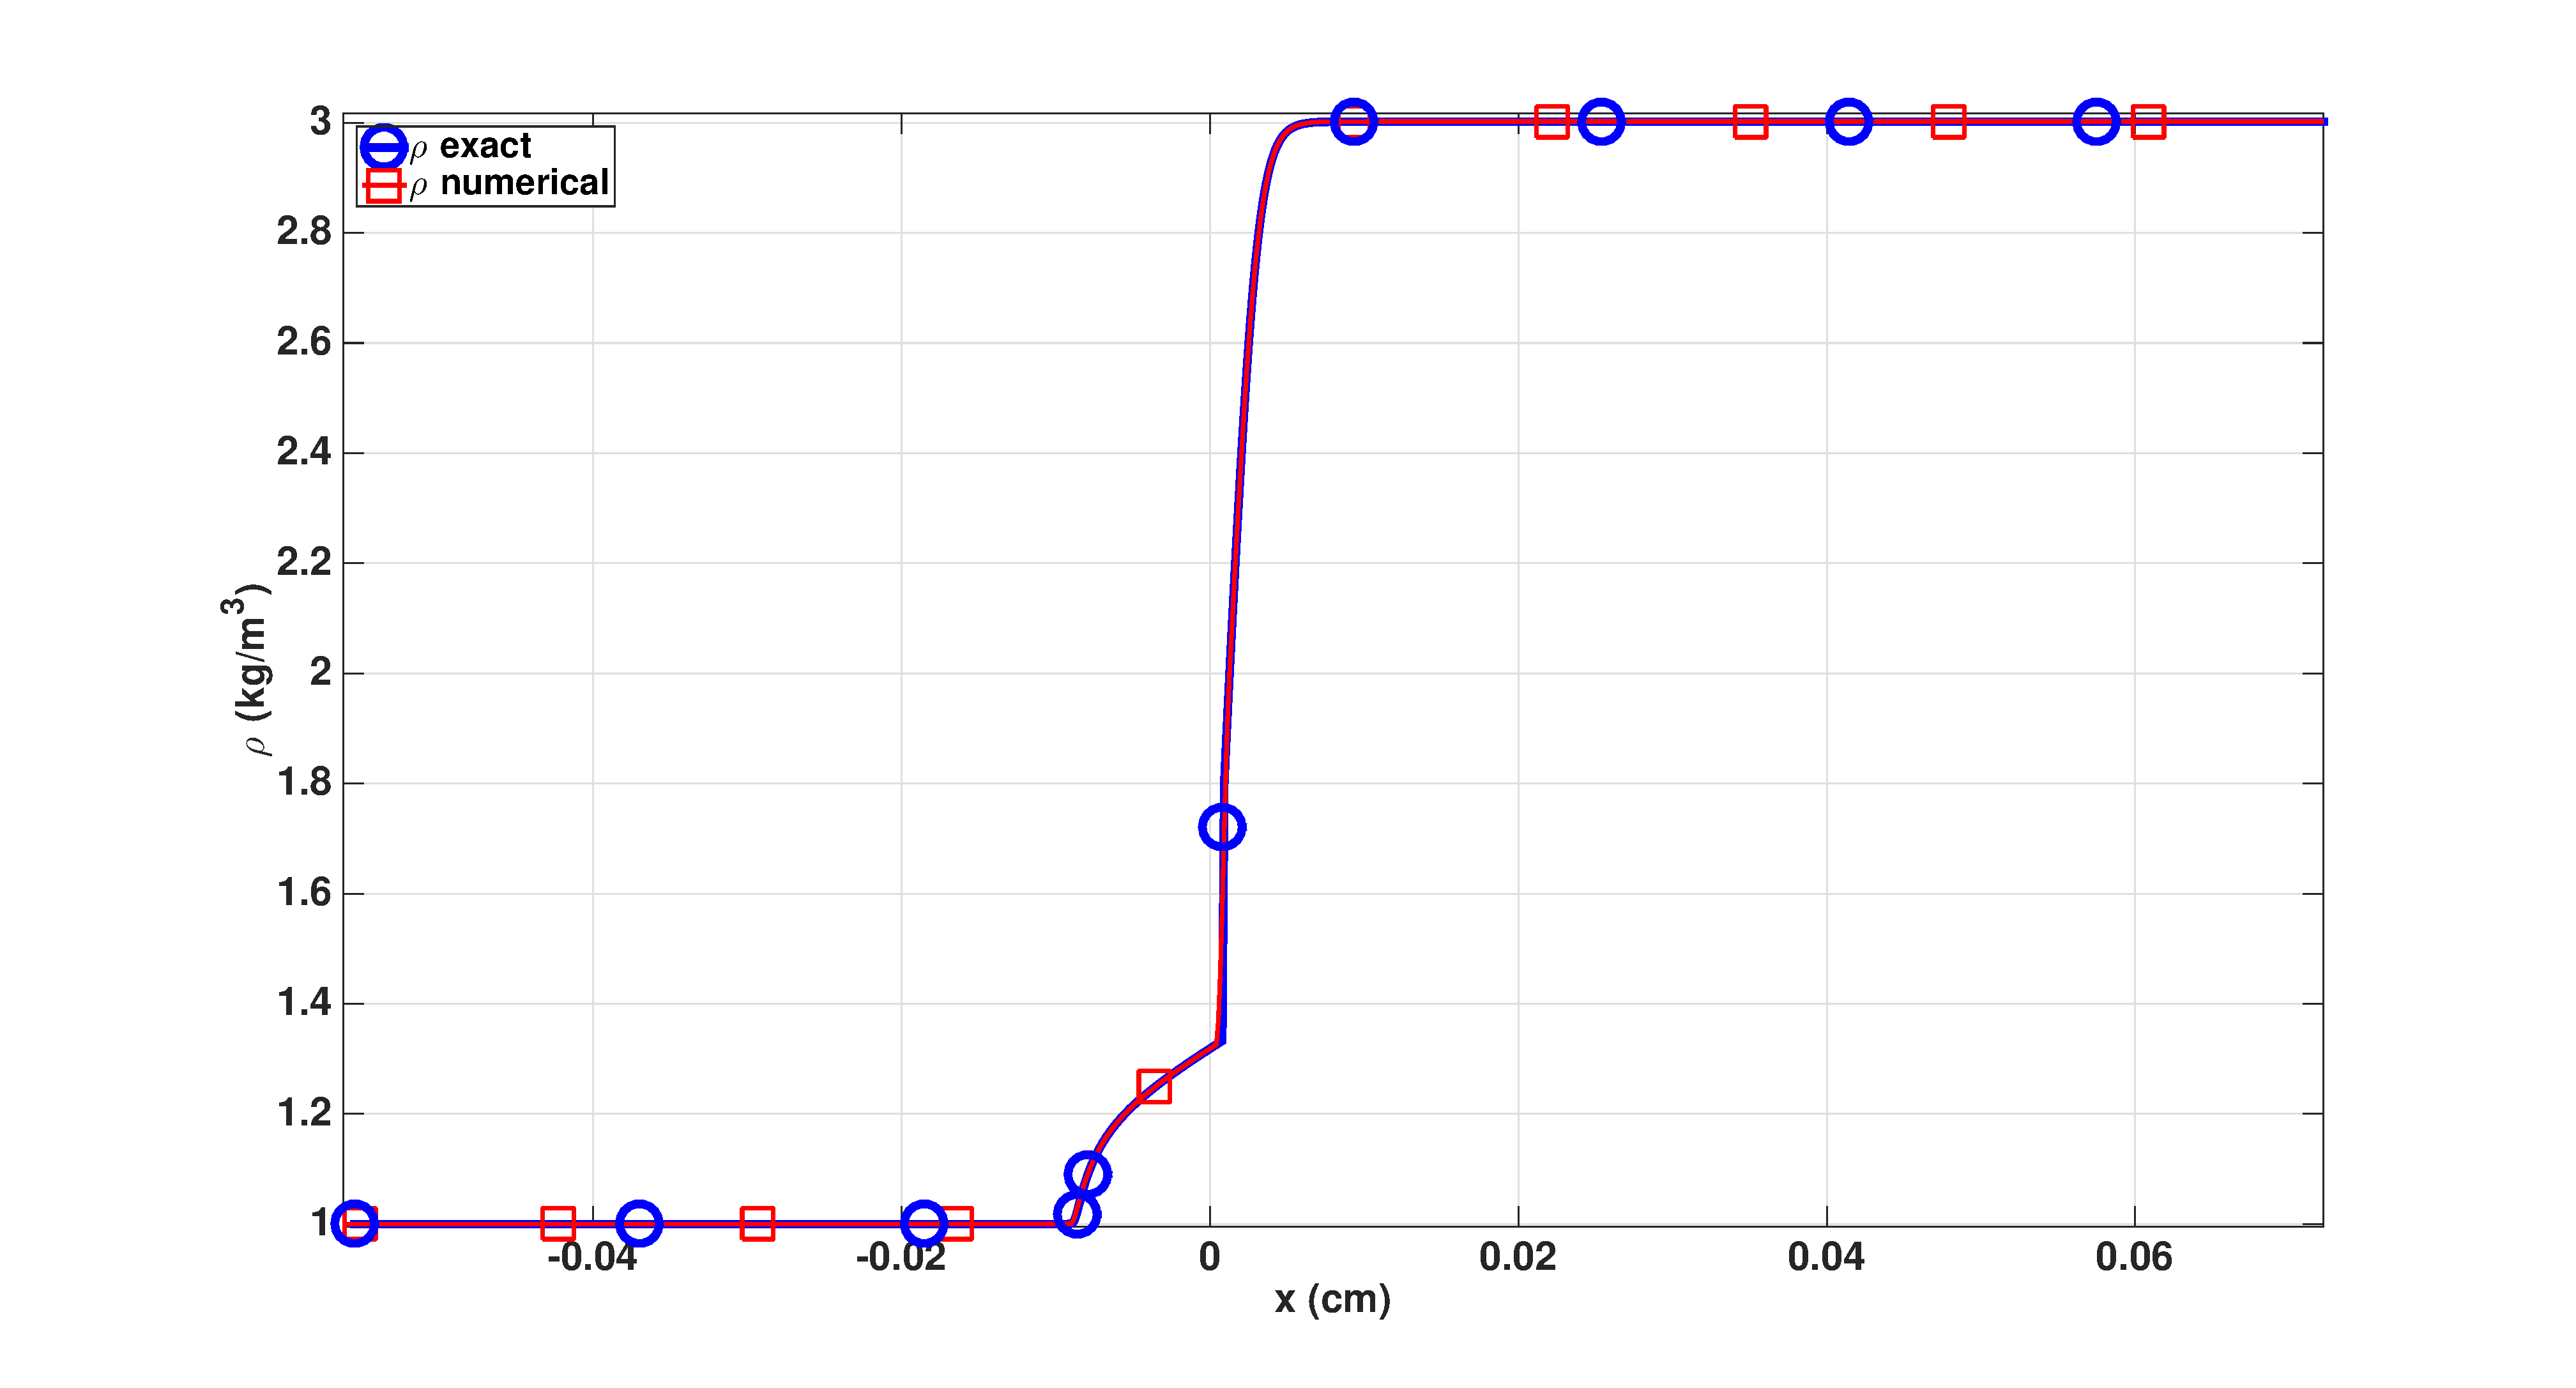
\includegraphics[width=\textwidth]{figures/dpt-xs/mach_3_nel_1000_density.eps}
    \caption{Steady-state material density for the Mach-3 shock test with temperature-dependent opacities.}\label{fig:mach-3-dpt-xs-dens}
\end{figure}
%
The density profile plotted in \fig{fig:mach-3-dpt-xs-dens} does not show any instability neither in the vicinity of the shock around $x = 0 \ cm$ nor in the abrupt change located at $x = -0.01 \ cm$. The shock is well resolved and the numerical and semi-analytical solutions overlap and are in excellent agreement.
%
\begin{figure}[H]
    \centering
    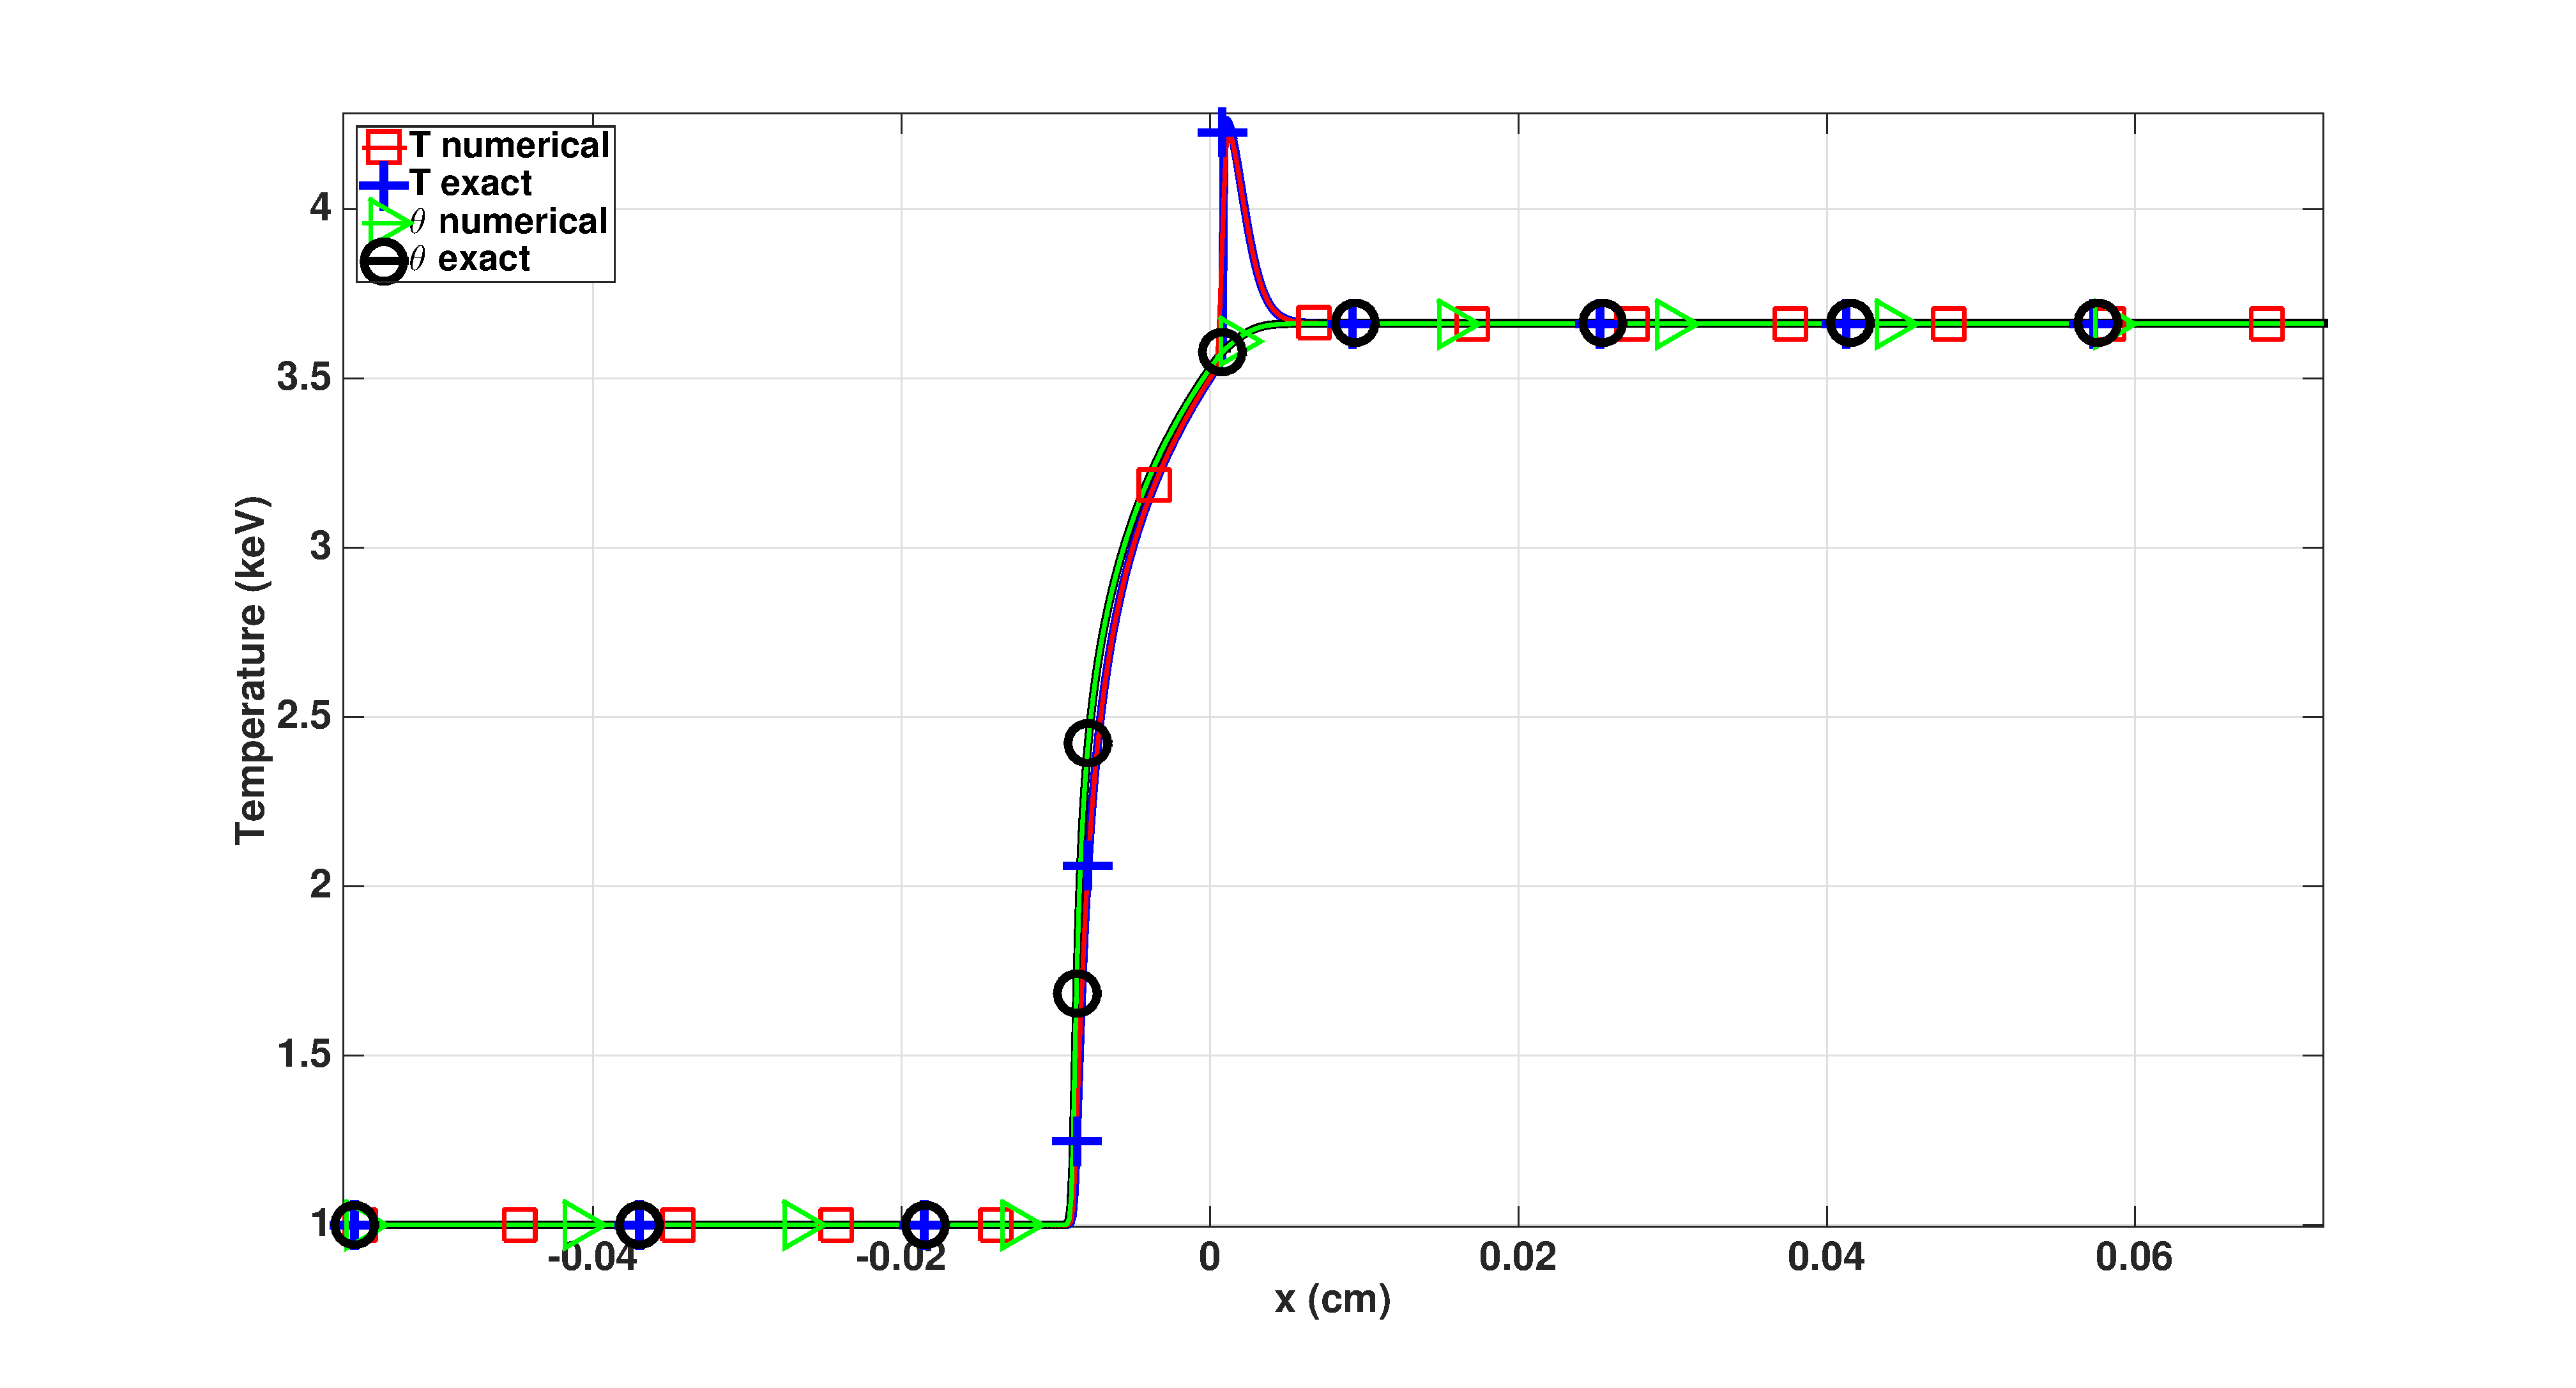
\includegraphics[width=\textwidth]{figures/dpt-xs/mach_3_nel_1000_temperature.eps}
    \caption{Steady-state material and radiation temperatures for the Mach-3 shock test with temperature-dependent opacities.}\label{fig:mach-3-dpt-xs-temp}
\end{figure}
%
In \fig{fig:mach-3-dpt-xs-temp}, the material and radiation temperatures do not show any instability either. The Zeldovich's pike in the material temperature profile is well resolved. The radiation temperature remains smooth as expected because of the diffusion term in the radiation equation. The numerical and semi-analytical solutions are in excellent agreement. 
%
\begin{figure}[H]
    \centering
    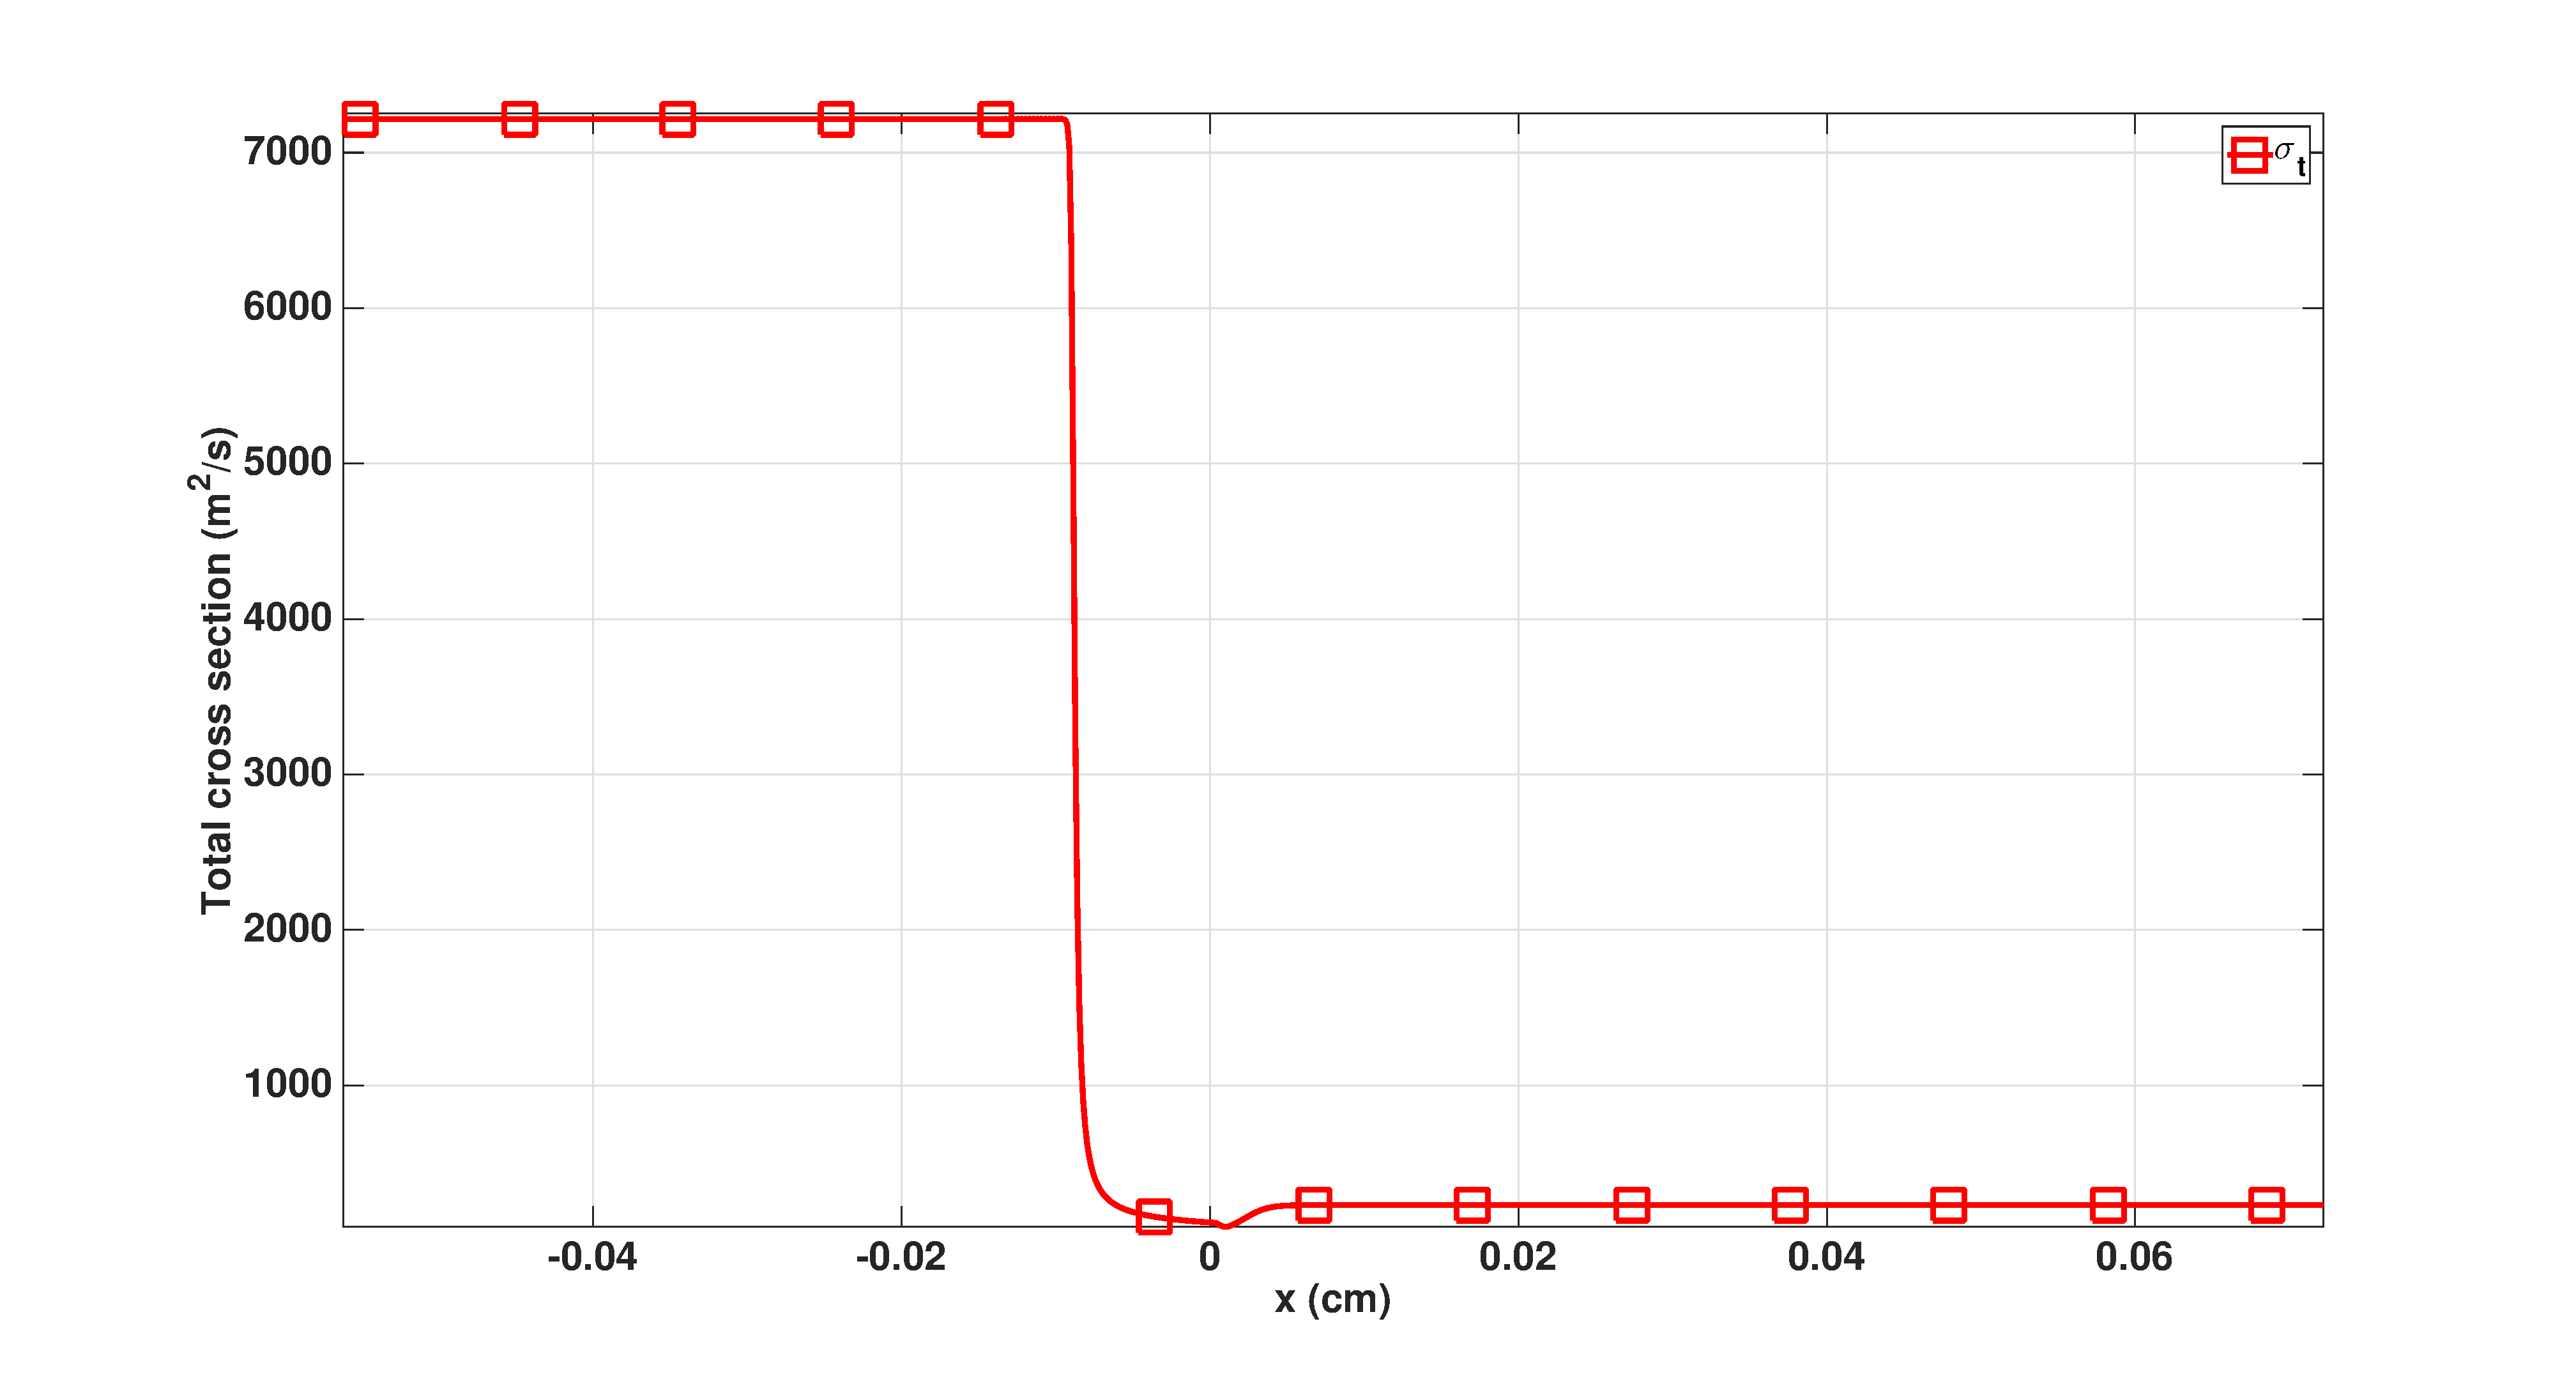
\includegraphics[width=\textwidth]{figures/dpt-xs/mach_3_nel_1000_total_cross_section.eps}
    \caption{Steady-state total opacity $\sigma_t$ for the Mach-3 shock test with temperature-dependent opacities.}\label{fig:mach-3-dpt-xs-xs}
\end{figure}
%
The numerical profile of the cross section is plotted in \fig{fig:mach-3-dpt-xs-xs} against the semi-analytical solution that was computed from the semi-analytical solutions of the material density and temperature. 
%We recall here that the material is a pure absorber and thus, the total and absorption cross sections are equal. The cross section varies by a factor $30$ in the shock region which .... \tcb{Are we not in the case where the material is optically thick in the pre-shock region? If this is the case, we should write something about the interest of using the local entropy residual with a local normalization as we do for Euler equation.}
%
\begin{figure}[H]
    \centering
    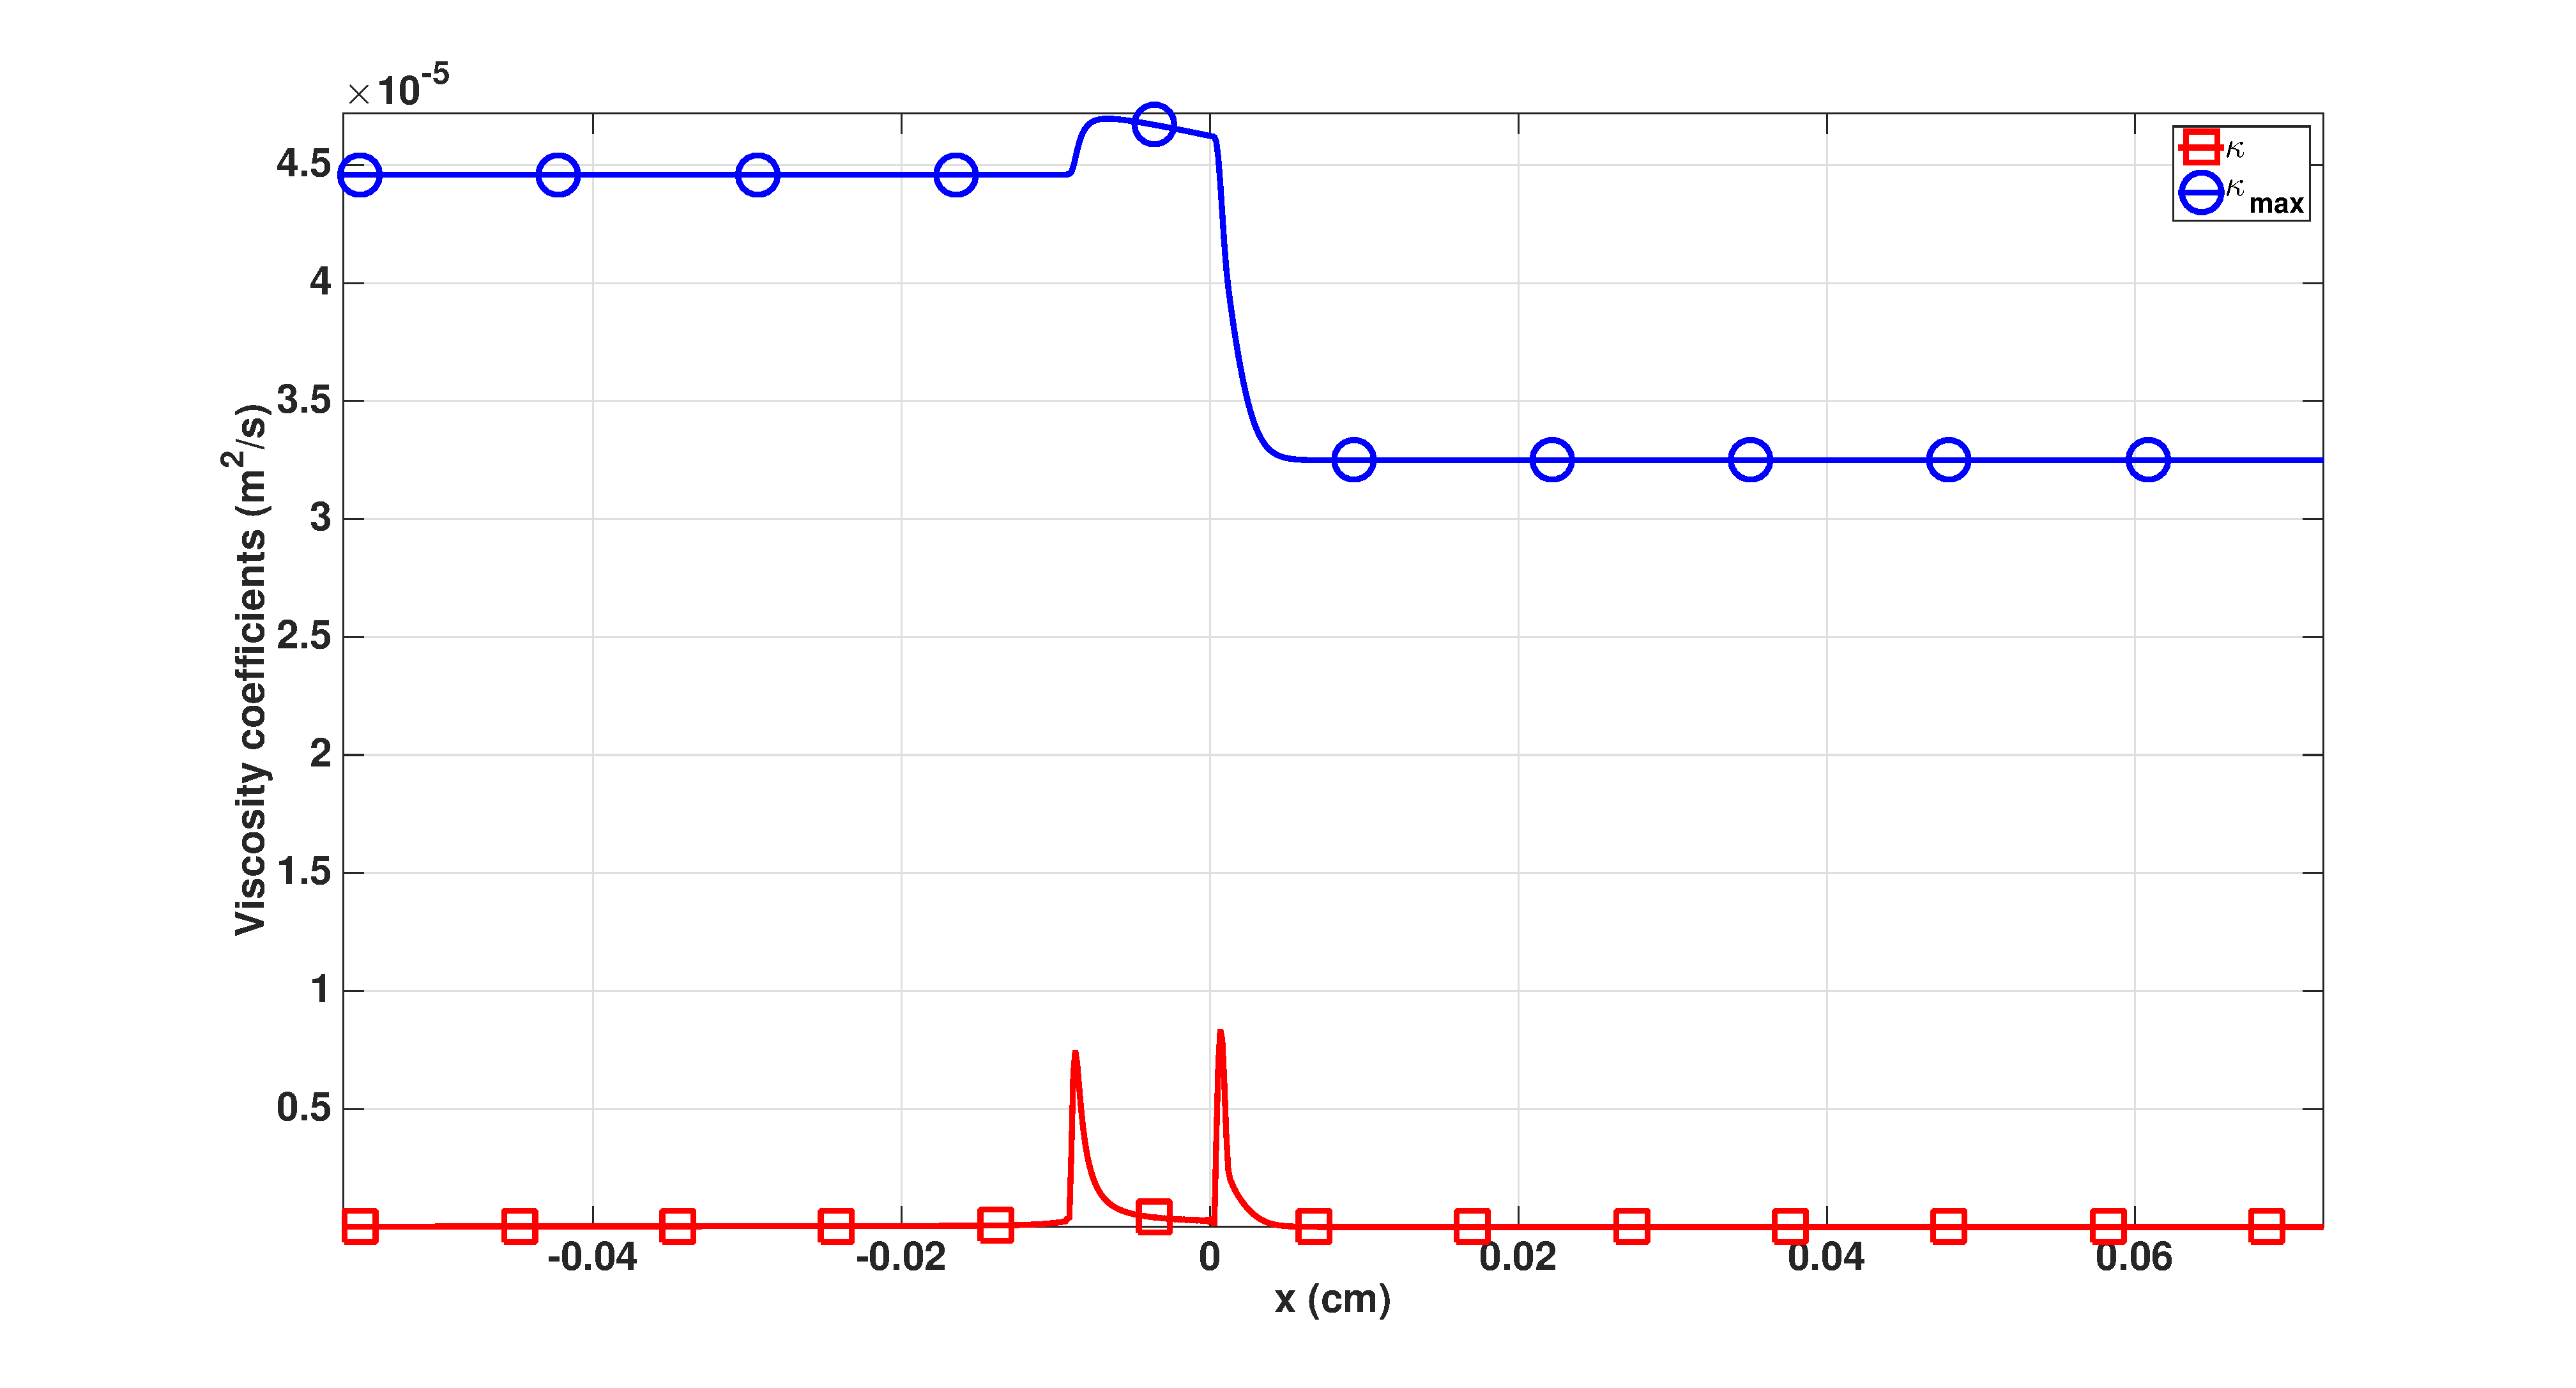
\includegraphics[width=\textwidth]{figures/dpt-xs/mach_3_nel_1000_viscosity.eps}
    \caption{Steady-state solution of the artificial viscosity coefficients for the Mach-3 shock test with temperature-dependent opacities.}\label{fig:mach-3-dpt-xs-visc}
\end{figure}
%
%\tcb{Shall we add a plot of the material density profile run without the jumps for comparison?} \\ 
The profiles of the entropy- ($\kappa_e$) and first-order ($\kappa_{max}$) viscosity coefficients are showed in \fig{fig:mach-3-dpt-xs-visc}. We observe that the entropy viscosity coefficient $\kappa_e$ displays two peaks at $x=-0.01 \ cm$ and at $x = 0 \ cm$. The latter one coincides with the shock position where the entropy residual $R_e(x,t)$ is known to be peaked. % (see \sct{sec:def-visc-coeff} and also \cite{our_jcp_radhy_paper}). 
The former one, is due to the inclusion of the jumps in the definition of the entropy viscosity coefficient as shown in \eqt{eq:equation12} and \eqt{eq:equation13}: the material density does not experience a shock at $x=-0.01 \ cm$ but a sharp variation that triggers a larger  jump value. 
%It is also observed that the entropy viscosity coefficient $\kappa_e$ does not saturate to the first-order viscosity coefficient $\kappa_{max}$ in the vicinity of the shock around $x = 0 \ cm$ which can be explained by the dissipative behavior of the source terms that add dissipation as highlighted in \sct{sec:VR_new}. 
Overall, the entropy viscosity coefficient behaves as expected: it is peaked in the vicinity of the shock and in regions of sharp variations, and small elsewhere.
%
%------------------------------------------------------------------
%------------------------------------------------------------------
\section{Conclusions and future work}
%------------------------------------------------------------------
%------------------------------------------------------------------
In this paper, the theoretical foundation for the application of the entropy viscosity method to the full non-equilibrium Grey Radiation Hydrodynamic equations, i.e., including relaxation and source terms, has been strengthened, utilizing the notions of weak solution and entropy condition for non-conservative hyperbolic systems of equations. We show that 
(i) we still recover an entropy condition that holds for the full GRH equations when borrowing the functional expression of the entropy  $s(\rho,e,\varepsilon)$ previously derived by only considering the hyperbolic parts of the GRH \cite{our_jcp_radhy_paper}, and
(ii) the same viscous regularization can be employed to stabilize the GRH equations.
%  and, (iii) the asymptotic study of the GRH equations is still equivalent to the equilibrium-diffusion limit (EDL) equations.

Using the above theoretical results, the definition of the first-order and entropy-viscosity coefficients from \cite{our_jcp_radhy_paper} are shown to be still valid. We presented two Mach-3 radiative shock simulations, with constant and material-dependent opacities, and observed that the entropy viscosity method behaves very satisfactorily when compared against semi-analytical solutions. Physical features such as embedded hydrodynamic shocks and the Zeldovich spike are resolved accurately without spurious oscillations. The entropy viscosity coefficient is only peaked in the vicinity of the shock and in region of strong gradients, and remains small elsewhere, as expected. 
%
Future work will include extension to multi-dimensional simulations and the use of an $S_n$ radiation transport approximation to model the radiation energy density distribution.



%%%%%%%%%%%%%%%%%%%%%%%%%%%%%%%%%%%%%%%%%%%%%%%%%%%%%%%%%%%%%
%%%%%%%%%%%%%%%%%%%%%%%%%%%%%%%%%%%%%%%%%%%%%%%%%%%%%%%%%%%%%
\section*{Acknowledgments}
The authors would like to acknowledge Jim Ferguson for providing the semi-analytical solutions and Jim Morel for many fruitful discussions. 
%%%%%%%%%%%%%%%%%%%%%%%%%%%%%%%%%%%%%%%%%%%%%%%%%%%%%%%%%%%%%
%%%%%%%%%%%%%%%%%%%%%%%%%%%%%%%%%%%%%%%%%%%%%%%%%%%%%%%%%%%%%


%%%%%%%%%%%%%%%%%%%%%%%%%%%%%%%%%%%%%%%%%%%%%%%%%%%%%%%%%%%%%
%%%%%%%%%%%%%%%%%%%%%%%%%%%%%%%%%%%%%%%%%%%%%%%%%%%%%%%%%%%%%

\bibliography{mybibfile}
\end{document}